\documentclass[whitelogo,11pt,a4paper]{tudelft-report}
\usepackage[english]{babel}
\hyphenation{an-iso-tropy}
\usepackage{amsmath}
\usepackage{amsfonts}
\usepackage{amssymb}
\usepackage{natbib}
%\usepackage[]{natbib}
\usepackage{changes}
\usepackage{pdfpages}
\usepackage{graphicx}
\usepackage{float}
\usepackage{subcaption}
\usepackage{rotate}
\usepackage{geometry}
\geometry{a4paper, total={170mm, 257mm}, left=20mm, right=20mm}
\usepackage[toc]{appendix}
%\usepackage[none]{hyphenat}  % wordbreak off
\usepackage{hyphenat}
\usepackage{hyperref}
%\hypersetup{breaklinks=true}
\usepackage{lipsum}
\usepackage{lineno}
\linenumbers
\numberwithin{equation}{chapter}
\graphicspath{{./Figures/}}
\usepackage{tikz}
\usetikzlibrary{shapes,snakes}
\setlength{\parindent}{0pt}   % no indents at textstart
\hypersetup{colorlinks=true,urlcolor=blue}
\urlstyle{same}
\usepackage{listings}
\usepackage{pythonhighlight}
\usepackage{cite}


\begin{document}

%% Use Roman numerals for the page numbers of the title pages and table of
%% contents.
\frontmatter

%% Uncomment following 19 lines for a cover with a picture
%\title[tudelft-white]{Title}
%\subtitle[tudelft-cyan]{Optional subtitle}
%\author[tudelft-white]{J.\ Random Author}
%\affiliation{Technische Universiteit Delft}
%\coverimage{cover.jpg}
%\titleoffsetx{10cm}
%\titleoffsety{10cm}
%\afiloffsetx{1cm}
%\afiloffsety{18cm}
%\covertext[tudelft-white]{
%    \textbf{Cover Text} \\
%    possibly \\
%    spanning 
%    multiple 
%    lines
%    \vfill
%    ISBN 000-00-0000-000-0
%}
%\makecover

%% Uncomment following 16 lines for a cover with a picture on the lower half only
%\font\headfont=cmr12 at 34pt
\title[tudelft-white]{Upscaling aquifer storage \\ and recovery (ASR)}
%\font\subfont=cmr12 at 26pt
\subtitle[tudelft-black]{A northern Ghana multiple case study \\ on small scale agriculture}
%\font\namefont=cmr12 at 22pt
\author[tudelft-white]{Frank J.\ van den Toorn}
\affiliation{Technische Universiteit Delft}
\coverimage{ASR_system.jpg}
\covertext[tudelft-white]{
    \textbf{} \\
%    covertext\\
%  	 possibly \\
%    spanning 
%    multiple 
%    lines
    \vfill
%    ISBN 000-00-0000-000-0
    }
\setpagecolor{tudelft-cyan}
%\makecover[split]

%\setkeys{Gin}{draft=true}        %plaatjes wel of niet inladen (false is aan, true is uit) en werkt ook opvolgend aan en uit per hoofdstuk bijvoorbeeld. 

%% Include an optional title page.
\begin{titlepage}


\begin{center}

%% Insert the TU Delft logo at the bottom of the page.
 
%% Print the title in cyan.
{\makeatletter
%\largetitlestyle\fontsize{32}{32}\selectfont\@title
\largetitlestyle\color{tudelft-cyan}\fontsize{32}{32}\selectfont\@title
\makeatother}

\bigskip
\bigskip

%% Print the optional subtitle in black.
{\makeatletter
\ifx\@subtitle\undefined\else
    \bigskip
   {\tudsffamily\fontsize{20}{20}\selectfont\@subtitle} \\
   %{\huge\tudsffamily\selectfont\@subtitle}     
    %\titlefont\titleshape\LARGE\@subtitle
\fi
\makeatother}

\bigskip
\bigskip

by
%door

\bigskip
\bigskip

%% Print the name of the author.
{\makeatletter
%\largetitlefont\Large\bfseries\@author
\largetitlestyle\fontsize{16}{16}\selectfont\@author
\makeatother}

\bigskip
\bigskip

to obtain the degree of Master of Science
%ter verkrijging van de graad van Master of Science

at the Delft University of Technology,
%aan de Technische Universiteit Delft,

to be defended publicly on .. August .., 2018 at ..:.. AM.
%in het openbaar de verdedigen op dinsdag 1 januari om 10:00 uur.

\vfill

\begin{tabular}{lll}
    Student number: & 4179404 \\
    Project duration: & \multicolumn{2}{l}{September 18, 2017 -- August .., 2018} \\
    Thesis committee: & Prof.\ dr.\ ir.\ M.\ Bakker, & TU Delft (Chair) \\
		& Prof.\ dr.\ ir.\ N.C.\ van de Giesen, & TU Delft \\        
        & Dr.\ ir.\ J.S.\ Timmermans, & TU Delft \\
        & Ir.\ D.A.\ Brakenhoff, & Witteveen+Bos
\end{tabular}
%% Only include the following lines if confidentiality is applicable.

\bigskip
\bigskip
%\emph{This thesis is confidential and cannot be made public until December 31, 2013.}
%\emph{Op dit verslag is geheimhouding van toepassing tot en met 31 december 2013.}

\bigskip
\bigskip
An electronic version of this thesis is available at \url{http://repository.tudelft.nl/}.
%\\[1cm]

%\centering{
\includegraphics{cover/logo_black}}


\end{center}

\begin{tikzpicture}[remember picture, overlay]
    \node at (current page.south)[anchor=south,inner sep=0pt]{
        
\includegraphics{cover/logo_black}
    };
\end{tikzpicture}

\end{titlepage}


\chapter*{Preface}
\setheader{Preface}
This thesis accommodates the final product in becoming a Master of Science in Watermanagement at the Delft University of Technology \-- faculty of Civil Engineering and Geosciences. I would like to acknowledge all the people who contributed to my graduation. Some deserve special emphasis. First of all, I would like to thank the entire committee for assessing my thesis. Subsequently, I would like to give a word of gratitude to Witteveen+Bos \-- Herman Mondeel \& Davíd Brakenhoff \-- for the research facilities and daily supervision. And, last but not least, I owe Conservation Alliance (CA) \-- Paa Kofi Osei-Owusu \-- a special gratitude. Without the cooperation of CA, the fieldwork data collection within the northern Ghana local communities would not have been possible.  


\begin{flushright}
{\makeatletter\itshape
    \@author \\
    Delft, August 2018
\makeatother}
\end{flushright}

\bigskip

%\begin{figure}
% \centering
% 
\includegraphics[width=0.9\linewidth]{TU_Delft_logo_RGB}
% %\caption{..}
% \label{fig:TUlogo}
%\end{figure}
% 
%\begin{figure}
% \centering
% 
\includegraphics[width=0.9\linewidth]{WitteveenBos_logo}
% %\caption{..}
% \label{fig:WBlogo}
%\end{figure}
% 
%\begin{figure}
% \centering
% 
\includegraphics[width=0.9\linewidth]{CA_logo}
% %\caption{..}
% \label{fig:CAlogo}
%\end{figure}

 
\begin{figure}[ht]
	\centering
	\begin{subfigure}[a]{0.33\linewidth}
		
\includegraphics[width=\linewidth]{TU_Delft_logo_RGB}
		%\caption{..}
		\label{fig:TUlogo}
	\end{subfigure}\vfill
	\begin{subfigure}[b]{0.33\linewidth}
        
\includegraphics[width=\linewidth]{WitteveenBos_logo}
		%\caption{..}
		\label{fig:WBlogo}
		\bigskip
		\bigskip
	\end{subfigure}\vfill
	\begin{subfigure}[c]{0.33\linewidth}
		
\includegraphics[width=\linewidth]{CA_logo}
		%\caption{..}
		\label{fig:CAlogo}	
	\end{subfigure} 
\end{figure} 

\chapter*{Summary}
\setheader{Summary}


Work In Progress. Summary will follow. \\

\tableofcontents
\listoffigures
\listoftables

%% Use Arabic numerals for the page numbers of the chapters.
\mainmatter

%%%\chapter{Introduction}

This document is intended to be both an example of the TU Delft \LaTeX{} template for reports and theses, as well as a short introduction to its use. It is not intended to be a general introduction to \LaTeX{} itself,\footnote{We recommend \url{http://en.wikibooks.org/wiki/LaTeX} as a reference and a starting point for new users.} and we will assume the reader to be familiar with the basics of creating and compiling documents.

Instructions on how to use this template under Windows and Linux, and which \LaTeX{} packages are required, can be found in \texttt{README.txt}.

\section{Document Structure}

Since a report, and especially a thesis, might be a substantial document, it is convenient to break it up into smaller pieces. In this template we therefore give every chapter its own file. The chapters (and appendices) are gathered together in \texttt{report.tex}, which is the master file describing the overall structure of the document. \texttt{report.tex} starts with the line
\begin{quote}
    \texttt{\textbackslash documentclass\{tudelft-report\}}
\end{quote}
which loads the TU Delft report template. The template is based on the \LaTeX{} \texttt{book} document class and stored in \texttt{tudelft-report.cls}. The document class accepts several comma-separated options. The default language is English, but this can be changed to Dutch (\emph{e.g.}, for bachelor theses) by specifying the \texttt{dutch} option:
\begin{quote}
    \texttt{\textbackslash documentclass[dutch]\{tudelft-report\}}
\end{quote}
Furthermore, hyperlinks are shown in blue, which is convenient when reader the report on a computer, but can be expensive when printing. They can be turned black with the \texttt{print} option. This will also turn the headers black instead of cyan.

If the document becomes large, it is easy to miss warnings about the layout in the \LaTeX{} output. In order to locate problem areas, add the \texttt{draft} option to the \texttt{\textbackslash documentclass} line. This will display a vertical bar in the margins next to the paragraphs that require attention. Finally, the \texttt{nativefonts} option can be used to override the automatic font selection (see below).

This template has the option to automatically generate a cover page with the \texttt{\textbackslash makecover} command. See the next section for a detailed description.

The contents of the report are included between the \texttt{\textbackslash begin\{document\}} and \texttt{\textbackslash end\{document\}} commands, and split into three parts by
\begin{enumerate}
\item\texttt{\textbackslash frontmatter}, which uses Roman numerals for the page numbers and is used for the title page and the table of contents;
\item\texttt{\textbackslash mainmatter}, which uses Arabic numerals for the page numbers and is the style for the chapters;
\item\texttt{\textbackslash appendix}, which uses letters for the chapter numbers, starting with `A'.
\end{enumerate}
The title page is defined in a separate file, \emph{e.g.}, \texttt{title.tex}, and included verbatim with \texttt{\textbackslash input\{title\}}.\footnote{Note that it is not necessary to specify the file extension.} Additionally, it is possible to include a preface, containing, for example, the acknowledgements. An example can be found in \texttt{preface.tex}. The table of contents is generated automatically with the \texttt{\textbackslash tableofcontents} command. Chapters are included after \texttt{\textbackslash mainmatter} and appendices after \texttt{\textbackslash appendix}. For example, \texttt{\textbackslash input\{chapter-1\}} includes \texttt{chapter-1.tex}, which contains this introduction.

The bibliography, finally, is generated automatically with
\begin{quote}
    \texttt{\textbackslash bibliography\{report\}}
\end{quote}
from \texttt{report.bib}. The bibliography style is specified in \texttt{tudelft-report.bst}, which is a modified version of \texttt{apsrev4-1.bst} (from REVTeX) designed to also display the titles of referenced articles. The template will automatically generate clickable hyperlinks if a URL or DOI (digital object identifier) is present for the reference. As an example, we cite the paper by Nobel laureate Andrei Geim and his pet hamster \citep{Geim2001}. Although it is possible to manage the bibliography by hand, we recommend using EndNote (available from Blackboard) or JabRef (available from \url{http://jabref.sourceforge.net/}).

\section{Cover and Title Page}

This template will automatically generate a cover page if you issue the \texttt{\textbackslash makecover} command. There are two formats for the cover page: one with a page-filling (`bleeding')
illustration, with the title(s) and author(s) in large ultrathin typeface, and the other where the illustration fills the lower half of the A4, whereas title(s), author(s) and additional
text are set in the standard sans-serif font on a plain background with a color chosen by the user. The last option is selected by the optional key \texttt{split}: \texttt{\textbackslash makecover[split]} yields
a page with the illustration on the lower half. All illustrations are bleeding, in accordance with the TU Delft style.

Before generating the cover, you need to provide the information to put on it. This can be done with the following commands:
\begin{itemize}
\item\texttt{\textbackslash title[Optional Color]\{Title\}} \\
    This command is used to provide the title of the document. The title
    title is also printed on the spine. If you use a title page (see below), this information will be used there as well.
    As the title, subtitle and author name are printed directly over the cover photo, it will often be necessary to adjust the print color in order to have
    sufficient contrast between the text and the background. The optional color argument is used for this.
\item\texttt{\textbackslash title[Optional Color]\{Subtitle\}} \\
    This command is used to provide a subtitle for the document. If you use a title page (see below), this information will be used there as well.
    It possible to adjust the print color in order to have
    sufficient contrast between the text and the background -- the optional color argument is used for this.
\item\texttt{\textbackslash author\{J.\ Random Author\}} \\
    This command specifies the author. The default color is \texttt{tudelft-white}, but this may be adjusted in the same way as the titles.
\item\texttt{\textbackslash affiliation\{Technische Universiteit Delft\}} \\
    The affiliation is the text printed vertically on the front cover. It can be the affiliation, such as the university or department name, or be used for the document type (\emph{e.g.}, Master's thesis). The default color is again \texttt{tudelft-white}, adjustable through the \texttt{color} option.
\item\texttt{\textbackslash coverimage\{cover.jpg\}} \\
    With this command you can specify the filename of the cover image. The image is stretched to fill the full width of the front cover (including the spine if a back cover is present).
\item\texttt{\textbackslash covertext\{Cover Text\}} \\
    If a back cover is present, the cover text is printed on the back. Internally, this text box is created using the \LaTeX{} \texttt{minipage} environment, so it supports line breaks.
\item\texttt{\textbackslash titleoffsetx\{OffsetX\},\textbackslash titleoffsety\{OffsetY\}}
    If the cover page contains a page-filling picture (i.e., \texttt{split} is not specified with the \texttt{makecover} command, the best position of the title depends a lot on the picture chosen for it. The lower left corner of the minipage containing title, subtitle and author is 
    specified by these two commands. The offsets are measured from the top left corner of the page. 
\item\texttt{\textbackslash afiloffsetx\{AfilX\}, \textbackslash afiloffsety\{AfilY\}}
    specifies the lower left corner of the text containing the affiliation, measured from the top left corner of the page. 
\end{itemize}

In addition to \texttt{[split]}, the \texttt{\textbackslash makecover} command accepts several additional options for customizing the layout of the cover. 
The most important of these is \texttt{back}. Supplying this option will generate a back cover as well as a front, including the spine. Since this requires a page size slightly larger than twice A4 (to make room for the spine), and \LaTeX{} does not support different page sizes within the same document, it is wise to create a separate file for the cover. \texttt{cover.tex} contains an example. The recommended page size for the full cover can be set with
\begin{quote}
    \textbackslash geometry\{papersize=\{1226bp,851bp\}\}
\end{quote}
after the document class and before \texttt{\textbackslash begin\{document\}}.

The other options \texttt{\textbackslash makecover} accepts are
\begin{itemize}
\item\texttt{nospine} \\
    If a back cover is generated, the title will also be printed in a black box on the spine. However, for smaller documents the spine might not be wide enough. Specifying this option disables printing the title on the spine.
\item\texttt{frontbottom} \\
    By default the black box on the front is situated above the blue box. Specifying this option will place the black box below the blue one.
\item\texttt{spinewidth} \\
    If a back cover is present, this option can be used to set the width of the spine. The default is \texttt{spinewidth=1cm}.
\item\texttt{frontboxwidth}, \texttt{frontboxheight}, \texttt{backboxwidth}, \texttt{backboxheight} \\
    As their names suggest, these options are used to set the width and height of the front (black) and back (blue) boxes. The default widths and heights are \texttt{4.375in} and \texttt{2.1875in}, respectively.
\item\texttt{x}, \texttt{y} \\
    The blue and black boxes touch each other in a corner. The location of this corner can be set with these options. It is defined with respect to the top left corner of the front cover. The default values are \texttt{x=0.8125in} and \texttt{y=3in}.
\item\texttt{margin} \\
    This option sets the margin between the borders of the boxes and their text. The default value is \texttt{12pt}.
\end{itemize}

For a thesis it is desirable to have a title page within the document, containing information like the thesis committee members. To give you greater flexibility over the layout of this page, it is not generated by a command like \texttt{\textbackslash makecover}, but instead described in the file \texttt{title.tex}. Modify this file according to your needs. The example text is in English, but Dutch translations are provided in the comments. Note that for a thesis, the title page is subject to requirements which differ by faculty. Make sure to check these requirements before printing.

\section{Chapters}

Each chapter has its own file. For example, the \LaTeX{} source of this chapter can be found in \texttt{chapter-1.tex}. A chapter starts with the command
\begin{quote}
    \texttt{\textbackslash chapter\{Chapter title\}}
\end{quote}
This starts a new page, prints the chapter number and title and adds a link in the table of contents. If the title is very long, it may be desirable to use a shorter version in the page headers and the table of contents. This can be achieved by specifying the short title in brackets:
\begin{quote}
    \texttt{\textbackslash chapter[Short title]\{Very long title with many words which could not possibly fit on one line\}}
\end{quote}
Unnumbered chapters, such as the preface, can be created with \texttt{\textbackslash chapter*\{Chapter title\}}. Such a chapter will not show up in the table of contents or in the page header. To create a table of contents entry anyway, add
\begin{quote}
    \texttt{\textbackslash addcontentsline\{toc\}\{chapter\}\{Chapter title\}}
\end{quote}
after the \texttt{\textbackslash chapter} command. To print the chapter title in the page header, add
\begin{quote}
    \texttt{\textbackslash setheader\{Chapter title\}}
\end{quote}

Chapters are subdivided into sections, subsections, subsubsections, and, optionally, paragraphs and subparagraphs. All can have a title, but only sections and subsections are numbered. As with chapters, the numbering can be turned off by using \texttt{\textbackslash section*\{\ldots\}} instead of \texttt{\textbackslash section\{\ldots\}}, and similarly for the subsection.
\section{\textbackslash section\{\ldots\}}
\subsection{\textbackslash subsection\{\ldots\}}
\subsubsection{\textbackslash subsubsection\{\ldots\}}
\paragraph{\textbackslash paragraph\{\ldots\}}
Lorem ipsum dolor sit amet, consectetur adipisicing elit, sed do eiusmod tempor incididunt ut labore et dolore magna aliqua. Ut enim ad minim veniam, quis nostrud exercitation ullamco laboris nisi ut aliquip ex ea commodo consequat. Duis aute irure dolor in reprehenderit in voluptate velit esse cillum dolore eu fugiat nulla pariatur. Excepteur sint occaecat cupidatat non proident, sunt in culpa qui officia deserunt mollit anim id est laborum.

\section{Fonts and Colors}

The fonts used by this template depend on which version of \LaTeX{} you use. Regular \LaTeX, \emph{i.e.}, if you compile your document with with \texttt{latex}, \texttt{pslatex} or \texttt{pdflatex}, will use Utopia for text, Fourier for math and Latin Modern for sans-serif and monospaced text. 
However, if you want to adhere to the TU Delft house style, you will need to use \XeLaTeX, as it supports TrueType and OpenType fonts. Compiling with \texttt{xelatex} will use Arial for most titles and text, Courier New for monospace and Cambria for math. If you want to haf a sans-serif font for the
main text, while using \texttt{latex}, \texttt{pslatex} or \texttt{pdflatex}, you can use the option \texttt{noroman} in the report style: \texttt{\textbackslash usepackage[\ldots,noroman]{tudelft-report}}. For document and part titles,  TU Delft Ultra Light is used. For quotes, columns and text in boxes, you use Georgia. If you want to use \XeLaTeX, but do not want to use the TU Delft house style fonts, you can add the \texttt{nativefonts} option to the document class. This will still use  TU Delft Utra Light and Arial on the cover, but not for the body of the document. If you need to use these fonts for certain sections in the main text, they are available via \texttt{\textbackslash tudrmfamily} (Georgia) and \texttt{\textbackslash tudtitlefamily} (TU Delft Utra Light).

\begin{quote}
  You have to learn the rules of the game. And then you have to play better than anyone else.\\
  \emph{Albert Einstein}
\end{quote}

The corporate colors of the TU Delft are cyan, black and white, available via \texttt{\textbackslash color\{{\color{tudelft-cyan}tudelft-cyan}\}}, \texttt{\textbackslash color\{{\color{tudelft-black}tudelft-black}\}} (which differs slightly from the default \texttt{\textbackslash color\{black\}}) and \texttt{\textbackslash color\{tudelft-white\}}, respectively. Apart from these three, the house style defines the basic colors \texttt{\color{tudelft-sea-green}tudelft-sea-green}, \texttt{\color{tudelft-green}tudelft-green}, \texttt{\color{tudelft-dark-blue}tudelft-dark-blue}, \texttt{\color{tudelft-purple}tudelft-purple}, \texttt{\color{tudelft-turquoise}tudelft-turquoise} and \texttt{\color{tudelft-sky-blue}tudelft-sky-blue}, as well as the accent colors \texttt{\color{tudelft-lavendel}tudelft-lavendel}, \texttt{\color{tudelft-orange}tudelft-orange}, \texttt{\color{tudelft-warm-purple}tudelft-warm-purple}, \texttt{\color{tudelft-fuchsia}tudelft-fuchsia}, \texttt{\color{tudelft-bright-green}tudelft-bright-green} and \texttt{\color{tudelft-yellow}tudelft-yellow}.


\chapter{Introduction}
\section{Northern Ghana characteristics}
Ghana’s northern part climate is labelled as semi-arid savannah-like. High temperatures are common and on a yearly basis the short rainy season is out-performed by long periods of drought. As a source of water supply, groundwater is abstracted from its surroundings. The relatively high-quality water is collected and mainly used for domestic purposes, livestock and construction. In more restricted quantities groundwater is used for irrigation. The use of groundwater prevents farmers from incurring potential losses in crop production and increases yields. \bigskip\\
For as long as natural recharge rates exceed discharge, the used groundwater is renewable and the water source is stated to be sustainable. It is roughly estimated the environment has the capability to naturally recharge a maximum of 2.5-10\% of the annual rainfall. Based on the rainfall data for northern Ghana this results in an estimated long term annual natural recharge of 60 mm/y. Currently, local groundwater use is estimated to be approximately 5\% of this annual recharge (Martin, 2006). The amount of water withdrawn is marginal and the environment is therefore self-reliant. However, fluctuations in groundwater use over time and place do occur. Accurate field data on these fluctuations is lacking. Recent observations show wells drying out and groundwater tables falling, both indicators of possible unsustainable groundwater use.
\bigskip\\
Following the trend seen in previous decades, it is expected future groundwater production will further increase. An overall improvement of the Ghanaian energy network as well as lower energy costs will make groundwater more accessible via electrical pumps. In general, this will lead to more extensive use of groundwater in the ongoing battle against shortages in clean drinking water. On top of this the national government aims at becoming more self-sufficient. Policies are pointed at more intensive agricultural development in the northern regions of Ghana (Wood, 2013). Optimization in field irrigation has the potential to increase yields and even double the number of crops produced per year (Owusu et al., 2017). Consequently, the need for groundwater abstraction becomes substantially higher. Climate change can potentially have a negative influence on the natural recharge. While the need will be higher, natural recharge volumes can become lower. In the near future it is possible that discharge rates will exceed natural recharge and the abstracting of groundwater is no longer sustainable. Objective of this research is to explore the possibilities of scaling up artificially managed aquifer recharge (MAR) for aquifer storage and recovery (ASR) to contribute towards the continued sustainable use of groundwater in the northern regions of Ghana. 

\section{ASR systems}
blabla
\begin{figure}[h!]
	\centering
	\begin{subfigure}[b]{0.5\linewidth}
		\centering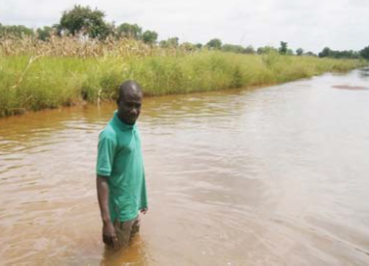
\includegraphics[width=0.8\linewidth]{Flood}
		\captionsetup{justification=centering}		
		\caption{\label{fig:Flood}}
		\end{subfigure}%\hfill
	\begin{subfigure}[b]{0.5\linewidth}
        \centering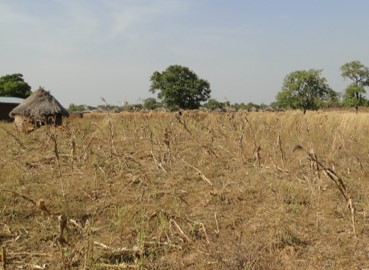
\includegraphics[width=0.8\linewidth]{Drought}
		\captionsetup{justification=centering}		
		\caption{\label{fig:Drought}}
		\end{subfigure}
		\captionsetup{justification=centering}	
	\caption[Example on (\subref{fig:Flood}) flood near Weisi, Upper West Region and (\subref{fig:Drought}) drought near Nungo, Upper East Region]{Example on (\subref{fig:Flood}) flood near Weisi, Upper West Region (source: Owusu et al., 2017) and (\subref{fig:Drought}) drought near Nungo, Upper East Region} 
	\label{fig:Flood_Drought}
\end{figure} \\

\begin{figure}[h]
 \centering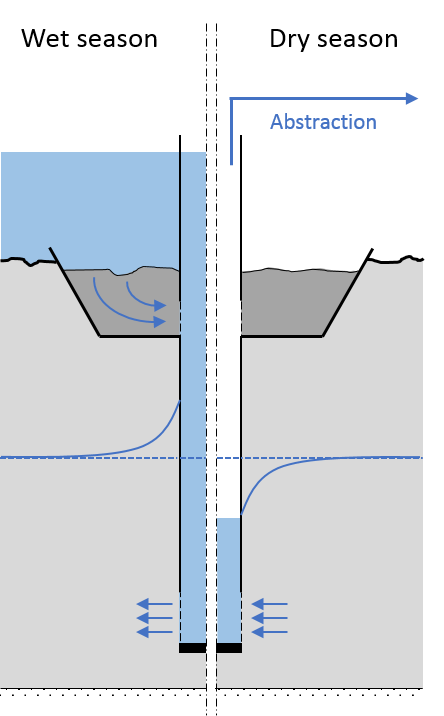
\includegraphics[width=0.4\linewidth]{Wet_Dry}
 \captionsetup{justification=centering}
 \caption{Principle Aquifer Storage \& Recovery (ASR) system}
 \label{fig:ASR}
\end{figure}

\section{PIT \& Irrigation purpose}
PIT application on irrigation (single figure). and the desired upscaling of this system (multiple figure). 

\begin{figure}[h]
 \centering
\includegraphics[width=0.8\linewidth]{Purpose}
 \captionsetup{justification=centering}
 \caption[Schematic: dry season system use]{Schematic: dry season system use \\ (visual support by Housin Aziz, Jhun Capaya and Nibras@design from Noun Project - \url{https://thenounproject.com})}
 \label{fig:Purpose}
\end{figure}

\begin{figure}[h]
 \centering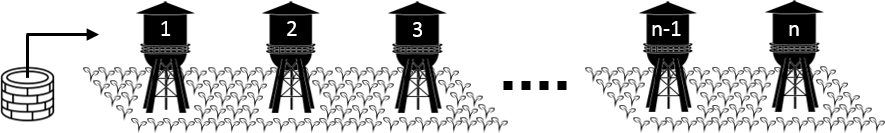
\includegraphics[width=0.8\linewidth]{Purpose_Multi}
 \captionsetup{justification=centering}
 \caption[Schematic: desired up-scaling in dry season system use]{Schematic: desired up-scaling in dry season system use \\ (visual support by Housin Aziz, Jhun Capaya and Nibras@design from Noun Project - \url{https://thenounproject.com})}
 \label{fig:Purpose_Multi}
\end{figure}

resulting in a research question

\textbf{Background}\

\textbf{Research gap}\

\textbf{Research purpose}\

\textbf{Research question}\

How can scaled-up Aquifer Storage and Recovery (ASR) systems be beneficial for the availability and sustainable use of agricultural groundwater in northern Ghana? \\

How can scaled-up Aquifer Storage and Recovery (ASR) systems be beneficial for the availability and sustainable use of groundwater in northern Ghana agriculture?

\textbf{Reader's guide}\
to answer this research question... 

%%%\chapter{Theoretical background}
tttttt

\section{Section}


\subsection{Subsection}


%%%\chapter{Northern Ghana study site characteristics}
Ghana Ghana \\ Ghana

\section{Section}


\subsection{Subsection}


\chapter{Fieldwork data analysis}
\label{Fieldwork_data_analysis}
Geological conditions are highly heterogeneous in northern Ghana. Subsurface characteristics vary at short mutual distances. Adequate and reliable information about local geohydrological conditions is preferably gathered through site-specific fieldwork. In this research perspective, multiple northern Ghana borehole locations are subjected to groundwater pumping tests. 
\bigskip \\
The NGO Conservation Alliance (CA) installed several PIT locations in the summer of 2016, in the Upper East and Northern Region. Pumping tests are performed at four of these boreholes. A fifth PIT borehole (in Ziong) is monitored to study how the ASR system is used by local farmers. The figure below shows a map  of the research locations in northern Ghana (Figure~\ref{fig:Overviewlocations}).
\bigskip 

\begin{figure}[ht]
 \centering
 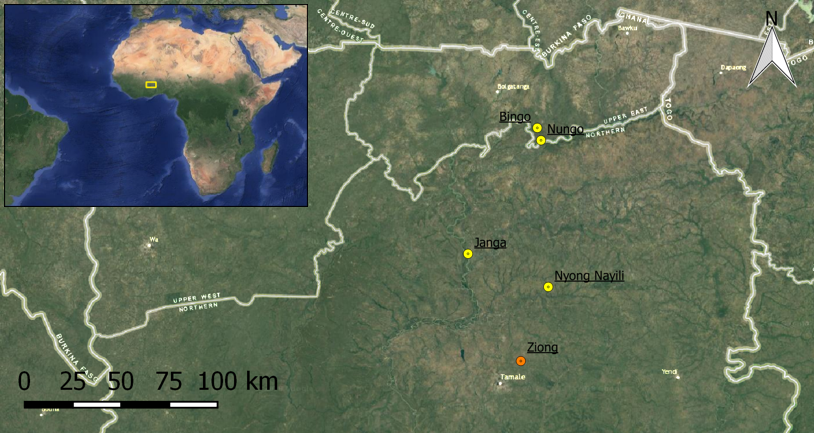
\includegraphics[width=\linewidth]{Overview_locations_northern_Ghana}
 \captionsetup{justification=centering} 
 \caption{Overview of fieldwork locations in northern Ghana}
 \label{fig:Overviewlocations}
\end{figure}

Detailed information on the equipment that was used, the set-up of the pumping tests as well as the monitoring of an operating ASR system can be found in appendix \ref{chapter:fieldwork_set-up}. The obtained raw fieldwork data can be found in the site-specific fact-sheets of appendix \ref{section:fieldworkresults}. The purpose of this fieldwork is to determine geohydrological subsurface parameters, transmissivity ($T$) and storativity ($S$), which are used as input for further investigation into upscaling these systems. 

This chapter contains the analysis of gathered fieldwork data. First, the methodology for data analysis, including some theoretical background, is explained (Section \ref{section:derivation_methods}). Section \ref{section:TS} contains the derivation of the local geohydrological parameter values: $T$ and $S$. Finally, the chapter concludes with the determination of parameter bandwidths (Section \ref{section:fieldwork_results}), which will be used in the subsequent model simulations. 

\section{Parameter derivation methods}
\label{section:derivation_methods}

\subsection{Theoretical model definition}
In large parts of northern Ghana the geohydrological soil characteristics are unknown. Strong variations at short mutual distance makes it necessary to obtain more information about local geology. The most reliable site-specific information was recorded during the drilling of boreholes (2016). The borehole log-sheets (appendix \ref{chapter:Borehole_logsheets}) are used as a starting point for the construction of the applied theoretical models in fieldwork analysis. 
\\

The site-specific borehole logsheets show similarities in stratification. In each case the upper 50 meters is divided into two or three layers, consisting of a confining top layer, and below that one or two "aquifers". Groundwater tables are predominantly positioned in the first aquifer. Based on these observations three simplified theoretical models for the analysis of fieldwork data are derived, as depicted in Figure \ref{fig:schematic_fieldwork_analysis}. 

\begin{figure}[h!]
	\centering
	\begin{subfigure}[b]{0.21\linewidth}
		\centering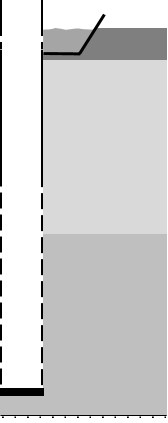
\includegraphics[width=0.6\linewidth]{Schematic_general_analysis}
		\captionsetup{justification=centering}		
		\caption{\label{fig:Schematic_general_analysis}}
		\end{subfigure}%\hfill
	\begin{subfigure}[b]{0.12\linewidth}
		\centering
\includegraphics[width=0.6\linewidth]{arrow_right}
		\end{subfigure}%\hfill
		%{\LARGE$\yrightarrow{}$}
	\begin{subfigure}[b]{0.21\linewidth}
		\centering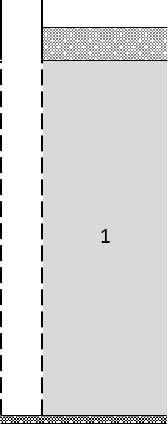
\includegraphics[width=0.6\linewidth]{Schematic_1lay_analysis}
		\captionsetup{justification=centering}		
		\caption{\label{fig:Schematic_1lay_analysis}}
		\end{subfigure}%\hfill
	\begin{subfigure}[b]{0.21\linewidth}
        \centering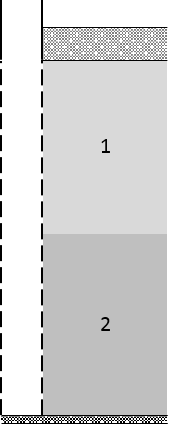
\includegraphics[width=0.6\linewidth]{Schematic_2lay_analysis}
		\captionsetup{justification=centering}		
		\caption{\label{fig:Schematic_2lay_analysis}}
		\end{subfigure}
	\begin{subfigure}[b]{0.21\linewidth}
        \centering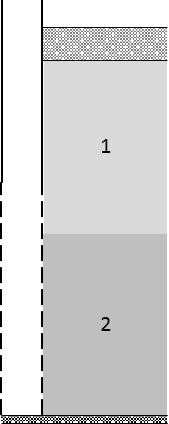
\includegraphics[width=0.6\linewidth]{Schematic_3lay_analysis}
		\captionsetup{justification=centering}		
		\caption{\label{fig:Schematic_3lay_analysis}}
		\end{subfigure}
	\captionsetup{justification=centering}	
	\caption{Schematic cross-sectional view of (\subref{fig:Schematic_general_analysis}) generalized northern Ghana soil stratification and simplified representations: (\subref{fig:Schematic_1lay_analysis}) a single layer system, ~(\subref{fig:Schematic_2lay_analysis}) a double layer system, and ~(\subref{fig:Schematic_3lay_analysis}) a system with two layers and partial penetration of the well} 
	\label{fig:schematic_fieldwork_analysis}
\end{figure} 

These simplified models (Figure \ref{fig:Schematic_1lay_analysis} - \ref{fig:Schematic_3lay_analysis}) mimic local conditions, making the derivation of representative hydraulic subsurface characteristics ($T$ and $S$) possible \citep{Kruseman2000}. Double layered models are applied to provide more degrees of freedom, potentially generating more accurate simulations. A maximum of two soil layers are implemented to limit chances of equifinality, due to an abundance of degrees of freedom. \\ 

\subsection{Techniques in analysis}
\label{section:techniques_analysis}
This section contains a description of the (analytical) models and methods used for optimal groundwater parameter estimation. \\


\textbf{Theis's method} \\ 
Groundwater drawdown due to the withdrawal of water can be determined analytically with Theis's equation (Equation \ref{eq:theis}). Theis's method is applicable on the situation depicted in \ref{fig:Schematic_1lay_analysis}; a constant rate pumping test in a fully penetrating well in a confined single layer aquifer \citep{Kruseman2000}. The analytical solution is suitable for obtaining a first indication of geohydrological parameters.   

\begin{equation}
\label{eq:theis}
 s = \frac{Q}{4\pi K D} exp1(u)
\end{equation}

\begin{equation}
 u = \frac{r^{2} S}{4 K D t}
\end{equation}

Where $s$ (m) is the drawdown at distance $r$ (m) from the well, $Q$ (m$^{3}$) is the constant well discharge , $KD$ (m$^{2}$/d) is the aquifer transmissivity ($KD$ = $T$), $S$ (-) is the aquifer storativity, $t$ (d) is the time measured from the start of pumping and $exp1$ is the exponential integral. The drawdown measurements in this research are limited to in-well measurements. The distance $r$ in Theis's equation is assumed to be the length of the well radius (0.0635 m). Theis's method is applicable for the time of pumping as well as the recovery process. The script below shows the implementation of Theis's method in Python.\\

\begin{python}[h!]
def drawdown(t, T, S):
    s = Qo / (4 * np.pi * T) * exp1(ro ** 2 * S / (4 * T *t))
    s[t > toff] -= Qo / (4 * np.pi * T) * exp1(ro ** 2 * S / (4 * T *(t[t>toff] - toff)))   
    return s
\end{python}

\textbf{Analytic Element Modelling in TTim}\\
TTim is a computer program based on analytic elements and designed for the analysis of transient groundwater flow in one or more layers. Multiple elements (and types of elements) can be added to specific predefined model layers. The use of TTim makes it possible to take additional well characteristics into account. Groundwater heads can be determined inside the well and the model optionally accounts for borehole storage and well skin resistance. Well discharge can be toggled on and off multiple times. This allows simulations of both single pumping and recovery tests and long-term well operations \citep{Mishra2013,Bakker2013}. \\

The analysis of the pumping and recovery tests is performed with the TTim \texttt{Model3D} configuration. The inclusion of a single well element is sufficient in this case. Depending on which subsurface model is used (Figure \ref{fig:schematic_fieldwork_analysis}) the well (analytic element) is screened in one or more model layers. The top layer is configured as phreatic layer, meaning the top layer storage coefficient ($S$) is a phreatic storage coefficient ($S_y$). This is based on observed initial groundwater tables, which are located below the bottom of the confining top layer. Multiplying this value with the aquifer thickness is therefore no longer needed. Each layer in the simplified model has a thickness of 1 meter. This means derived hydraulic conductivities ($k$) can be interpreted as transmissivities ($T$) and the storage is expressed as the layer storage coefficient ($S$). This is done to directly derive $T$ and $S$ values. Additionally, this approach automatically corrects for the unknown thickness of the deepest soil layer in which the well is screened. There is no information about soil conditions beyond the bottom of the wells in the borehole log-sheets (Appendix \ref{chapter:Borehole_logsheets}). \\

\textbf{MODFLOW}\\
The modelling of ASR upscaling scenario's (see Chapter \ref{chapter:model_scenarios}) is done with Modular Ground-Water Flow Model (MODFLOW), a finite difference model for groundwater flow developed by the U.S. Geological Survey (USGS). MODFLOW is the international standard in groundwater simulation (\citep{Niswonger2011,HarbaughArlen2005}). More information on the applied inputs can be found in Chapter \ref{chapter:model_scenarios}. In the case of fieldwork data analysis  MODFLOW is not used for the derivation of geohydrological parameters. Optimal parameters derived with TTim models are implemented in corresponding MODFLOW models to validate obtained TTim results.

\subsection{Optimization functions}
Pumping test data (section \ref{section:fieldwork_results}) is used as input for the derivation of local geohydrological parameter values. The values of $T$ and $S$ are determined by the method of (curve) fitting the analytical solutions and TTim models to the data. In this process two optimization functions are used. \\

\textbf{Fmin-RMSE optimization}\\
Differences between the measured and modelled drawdown curves can be expressed by the Root-Mean-Square-Error (Equation \ref{eq:RMSE}). The \texttt{Fmin} function (part of Python's \texttt{scipy.optimize} package) is applied to minimize the difference between modelled and observed drawdowns. This optimization results in optimal $T$ and $S$ values (and optionally values for borehole storage and well skin resistance) that represent local conditions. An example Python implementation of \texttt{Fmin} optimization is given below. It shows an optimization of five parameters ($T$ and $S$ values for two model layers and well skin resistance). \\ 

% example of monospace use: \texttt{hier wat je wilt hebben in monospace}!

\begin{equation}
\label{eq:RMSE}
 RMSE = \sqrt{\Sigma\frac{(s_{mod}-s_{field})^{2}}{N}}
\end{equation}

Where $s_{\text{mod}}$ is the modelled drawdown (m), $s_{\text{field}}$ is the observed drawdown (m) and N is the number of data points. \\
 
\begin{python}[h!]
def optimTTim_Qvar(params, t, meas):
    kaq = np.zeros(2)
    Saq = np.zeros(2)
    kaq[0] = params[0]             
    kaq[1] = params[1]
    Saq[0] = params[2]
    Saq[1] = params[3]
    res = params[4]
    s = drawdownTTim_Qvar(t, kaq, Saq, res)
    error = np.sqrt(np.mean((s-meas)**2)) 
    return error

xopt = fmin(optimTTim_Qvar, x0=[10, 10, .01, .001, 0.1], args=(to[mask], do[mask]), xtol=1e-4)
\end{python}
\bigskip

\textbf{Calibration function}\\
TTim has an in-built calibration function for the derivation of parameter values. Application of this second method improves the research robustness. In the Python script below, an example of the TTim \texttt{Calibrate} function is given. It is the same example as mentioned in the \texttt{Fmin} optimization above.\\ 

\begin{python}[h!]
cal = Calibrate(mlc)
cal.parameter(name='kaq0', layer=0, initial=10, pmin=0)
cal.parameter(name='kaq1', layer=1, initial=10, pmin=0)
cal.parameter(name='Saq0', layer=0, initial=.01, pmin=0, pmax=0.3)
cal.parameter(name='Saq1', layer=1, initial=.001, pmin=0, pmax=0.3)
cal.parameter(name='res', par=wc.res, initial=0.1)
cal.series(name='obs3', x=ro, y=0, layer=[0,1], t=to[mask], h=-do[mask])
cal.fit()
\end{python}

Both optimization methods require an initial estimate for the parameters. More than one suitable solution is possible, which makes the outcome of the optimization dependent on the choice of initial values. Other studies found that $T$ and $S$ values are commonly low in northern Ghana \citep[e.g.][]{Owusu2015,Owusu2017}. Based on these other studies the following initial conditions are applied: $k_{aq0}$ is 10 (m/d), $k_{aq1}$ is 10 (m/d), $S_{aq0}$ is 0.01 (-), $S_{aq1}$ is 0.001 (-) and well resistance is 0.1 (d). The actual well radius is used as the (initial) borehole storage: 0.0635 (m). Boundary conditions are applied to avoid the optimization resulting in physically improbable parameter values, i.e. negative parameter values and unnaturally high storativity values (greater than 0.3 (-)).

%(write something over initial conditions. Such small values. Not one single best solution. multiple 'best' solutions potentially close to each other. so solutions highly influential by the arbitrary chosen initial conditions. For each location several attempts done to see which initial conditions score pretty good. And subsequently generalization of those initial parameters applied per location/pumping test. for example better fit at Bingo at initial condition for T (KD) of 10, 10 (lay one and two) for fmin then for cal (2 layered system.) But 2 layered system all of sudden scores better with initial conditions 5, 1 for example.  

\section{From fieldwork data to $T$ \& $S$ values}
\label{section:TS}
The methods and models mentioned in the previous section are applied on the measurements from the five locations: Bingo, Nungo, Nyong Nayili, Janga and Ziong. Measurements results are included in the fact-sheets of Appendix \ref{section:fieldworkresults}. A complete overview of all optimization simulations (overall 25 per location) can be found in Appendix \ref{chapter:Extense_fieldwork_analysis}. Most important outcomes are discussed below for each of the five locations.

\subsection{Location: Bingo}

\textbf{Site inspection}\\
The surroundings of Bingo are characterized by a mildly sloping landscape. (Bed)rock appears occasionally at the surface. Site inspection showed an abundance of charred vegetation. The area is exposed to bush fires. As a consequence the agricultural field is not in operation. Map inspection shows the presence of the Volta river within several kilometres from Bingo. However, no indications of surface water (water-bodies and/or ponds) were observed. Bingo inhabitants label wet season flooding as high. Inundation levels of 1-2 m are common and usually last for several days. Flooding is not always caused by rain, every now and then a surplus of water accumulates at the surface by "popping up" out of ground. Inspection on the infiltration technology itself revealed the presence of a steel lid. Above surface level no well screen perforations were observed. The infiltration bed is an entrance path for the replenishment of groundwater.\\

\textbf{Measurement quality}\\
A malfunctioning power converter postponed the pumping test start. Since nightfall was a time limiting factor, the delay resulted in a shortened total test duration. In-well drawdown observation further downgraded the measurement quality. Well turbulence (due to pumping) caused the origin of a tangled rope. Hand measurements became more complicated and unreliable. An even more important consequence of the tangled rope was the occurrence of an undesirably high position of the deepest pressure sensor installed (see measurement set-up in Appendix \ref{section:measurement_structure}). Direct result is a long-term gap in pumping test drawdown data (yellow dotted line in Figure \ref{fig:Bingo_best}). The exact drawdown at the last moment of pumping is for example missing. Among other things due to the deliberate choice of a relative long-time recovery measurement the overall dataset can potentially be of use. \\

\textbf{Fit analysis} \\
The long-term absence of adequate data has its effects on the parameter fitting capabilities. As visible in Figure \ref{fig:Bingo_best}, Theis's method encounters difficulties here. Drawdown most definitely exceeded the measurement limit of 8m. This is not reflected in the parameter outcome of Theis's method. Defective fitting capabilities, due to a gab in data, are clearly less emphatically present in the analysis by the use of TTim.  Optimal parameter values are found at which drawdown curves exceed the drawdown measurement limit. Taking borehole storage and/or well resistance in consideration may potentially underlie this. This example shows it is not by definition required to feature complete drawdown data. By the use of TTim incomplete time series can result in adequate optimal parameter values. In order size the values found are low but align initial conditions. Furthermore it can be appointed that the double-layered transmissivity values found, suggest the presence of only one preferential layer of groundwater flow. \\

\begin{table}[h!]
\small
\centering
\caption{Bingo - overview best fit parameters}
\label{tab:bing_table}
\begin{tabular}{l|c|r|r|rr|rr|c}
\hline 
\textbf{}       & \textbf{Method} & \textbf{Stor [m]} & \textbf{Res [d]} & \textbf{T1}  & \textbf{T2   [m$^2$/d]}  & \textbf{S1}  & \textbf{S2 [-]}  & \textbf{RMSE [m]} \\ \hline \hline
Analytical                & fmin             & -             & -            & 10.83      & -          & 2.0e-04    & -          & 0.798 \\
1 lay                     & fmin             & 0.0647        & 5.6e-02      & 26.23      & -          & 6.6e-03    & -          & 0.163 \\
2 lay                     & fmin             & 0.0635        & -            & 2.8e-04    & 8.25      & 3.0e-03    & 2.1e-06    & 0.107 \\
2 lay (pp)                & fmin             & 0.0597        & -            & 8.6e-04    & 7.44      & 7.1e-03    & 6.3e-06    & 0.078 \\ \hline    
\end{tabular}
\end{table}

\begin{figure}[h!]
 \centering
 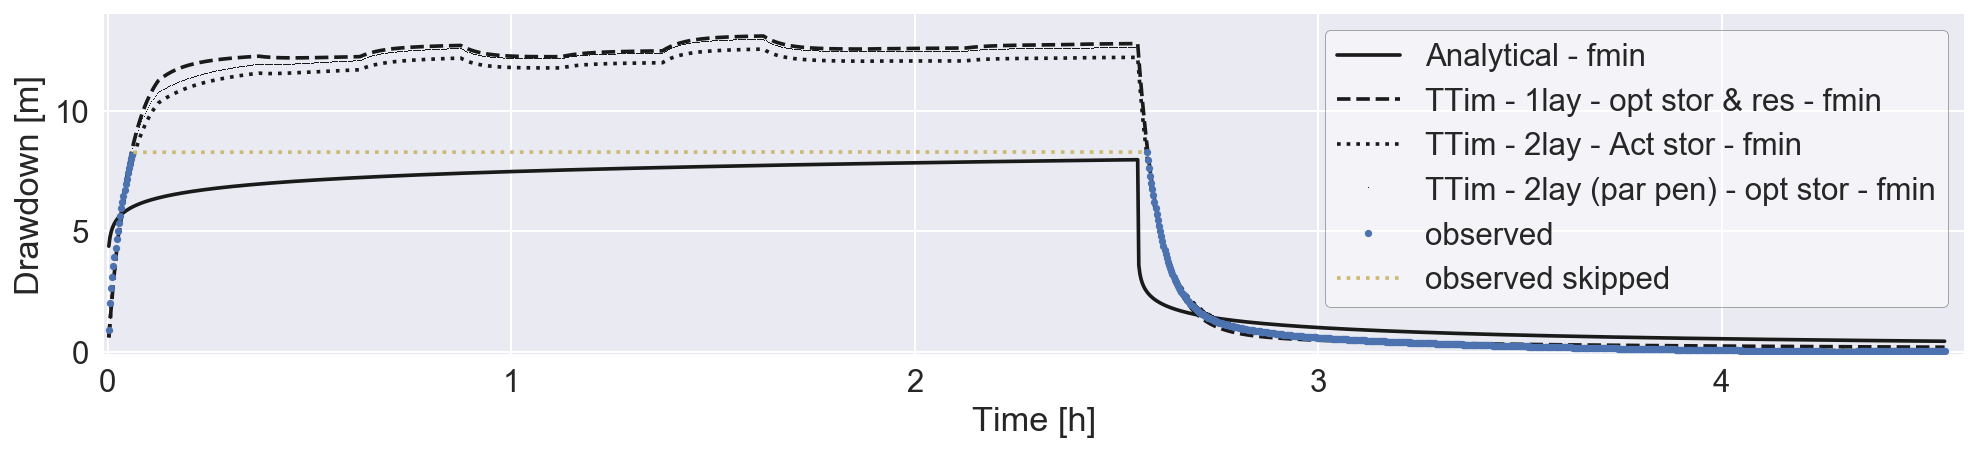
\includegraphics[width=\linewidth]{bingo_multi_lay_best}
 \captionsetup{justification=centering} 
 \caption{Bingo - Simplified models best fit}
 \label{fig:Bingo_best}
\end{figure}

\textbf{Substantive remark} \\
Both parameter optimization functions (\texttt{Fmin} and \texttt{Calibrate}) are able to derive reasonable solutions. Results of the \texttt{Calibrate}) optimization function reveal that an increase in model degrees of freedom not necessary leads to better performance (Appendix \ref{chapter:Extense_fieldwork_analysis}).Also by looking at the TTim best fit solutions (Figure \ref{fig:Bingo_best}) only minor distinction can be made in performance of the applied simplified models with a single layer, double layer or double layer with a partially penetrating well. Overall model accuracy slightly increases (Root-Mean-Square-Error slightly decreases) by an increase in complexity. An increase that can not be labelled as significant. All three simplistic theoretical models potentially represent nature properly by the in TTim found optimal parameters, depicted in Table \ref{tab:bing_table}.  

%\begin{figure}[h!]
%	\centering
%	\begin{subfigure}[b]{1\linewidth}
%		\centering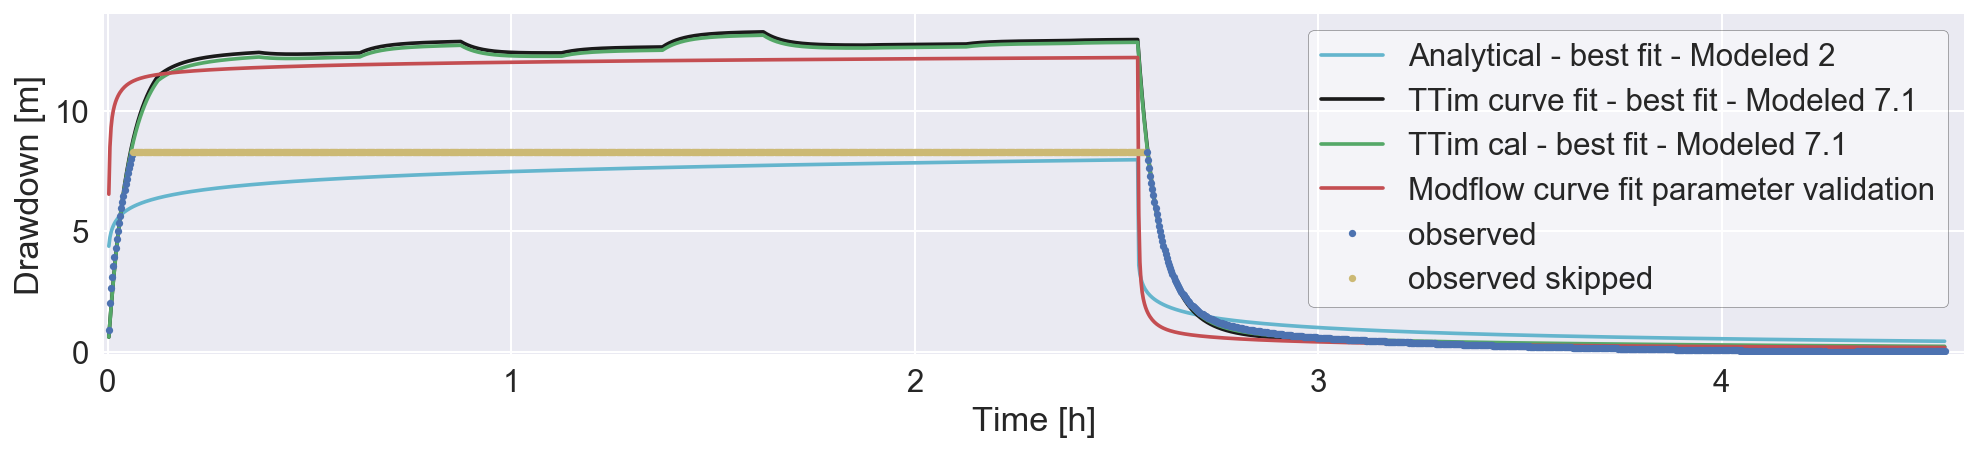
\includegraphics[width=1\linewidth]{bingo_1lay_analysis}
%		\captionsetup{justification=centering}		
%		\caption{\label{fig:bingo_1lay_analysis}}
%		\end{subfigure} \\ %\hfill
%	\begin{subfigure}[b]{1\linewidth}
%        \centering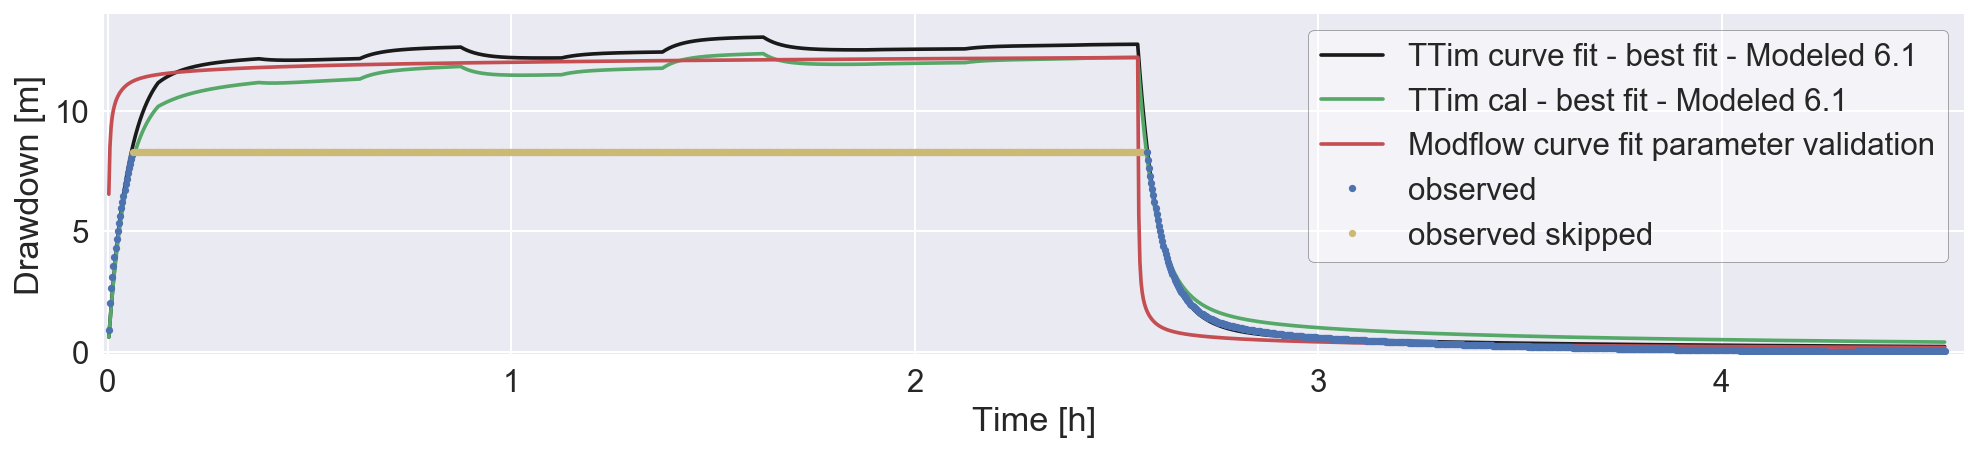
\includegraphics[width=1\linewidth]{bingo_2lay_analysis}
%		\captionsetup{justification=centering}		
%		\caption{\label{fig:bingo_2lay_analysis}}
%		\end{subfigure} \\
%	\begin{subfigure}[b]{1\linewidth}
%        \centering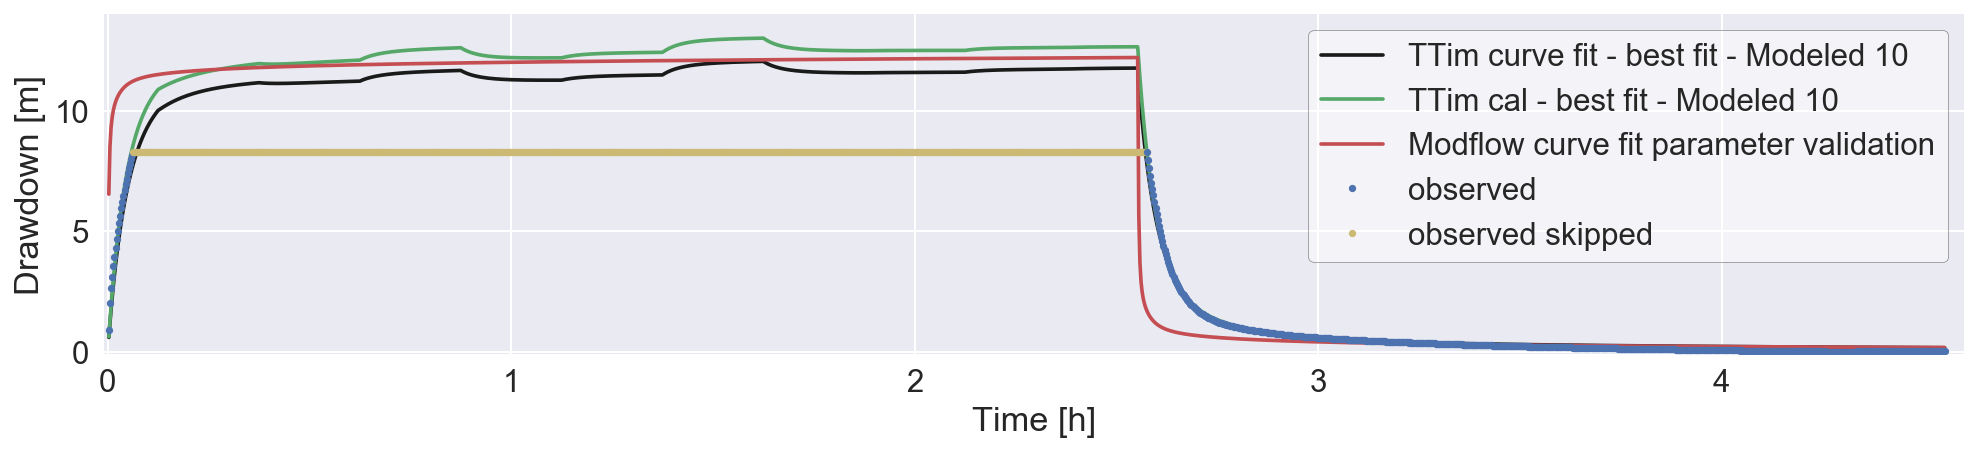
\includegraphics[width=1\linewidth]{bingo_3lay_analysis}
%		\captionsetup{justification=centering}		
%		\caption{\label{fig:bingo_3lay_analysis}}
%		\end{subfigure}
%	\captionsetup{justification=centering}	
%	\caption{Pumping test fit TS results: (\subref{fig:bingo_1lay_analysis}) single layered, ~(\subref{fig:bingo_2lay_analysis}) double layered and ~(\subref{fig:bingo_3lay_analysis}) triple layered (partially penetrating)} 
%	\label{fig:bingo_fieldwork_analysis}
%\end{figure} 

%
%\begin{table}[h!]
%\small
%\centering
%\caption{Bingo - overview best fit parameters}
%\label{tab:bingo_table}
%\begin{tabular}{l|l|l|lll|lll|l}
%\hline 
%\textbf{}       & \textbf{Stor [m]} & \textbf{Res [d]} & \textbf{T1}& \textbf{T2}  & \textbf{T3   [m$^2$/d]}  & \textbf{S1}& \textbf{S2}  & \textbf{S3 [-]}  & \textbf{RMSE [m]} \\ \hline
%\textbf{Single Lay}       & \textbf{} & \textbf{} & \textbf{}& \textbf{}& \textbf{}  & \textbf{}& \textbf{}& \textbf{}  & \textbf{}                    \\ \hline
%Analytical                & -             & -            & 10.83      & -          & -          & 2.0E-04    & -          & -          & 0.798         \\
%Curve fit                 & -             & 0.05         & 25.52      & -          & -          & 7.3E-05    & -          & -          & 0.166         \\
%Cal                       & -             & 2.5E-04      & 21.94      & -          & -          & 5.9E-19    & -          & -          & 0.175         \\
%{\textbf{}}               &               &              &            &            &            &            &            &            &               \\ 
%\textbf{Double Lay}       & \textbf{} & \textbf{} & \textbf{}& \textbf{}& \textbf{}  & \textbf{}& \textbf{}& \textbf{}  & \textbf{}                    \\ \hline
%Curve fit                 & -             & 0.06         & 22.88      & 0.40       & -          & 4.2E-04    & 8.0E-04    & -          & 0.167         \\
%Cal                       & -             & 0.02         & 11.63      & 0.57       & -          & 3.3E-07    & 4.7E-06    & -          & 0.413         \\ {\textbf{}}               &               &              &            &            &            &            &            &            &               \\ 
%\textbf{Triple Lay}       & \textbf{} & \textbf{} & \textbf{}& \textbf{}& \textbf{}& \textbf{}& \textbf{}& \textbf{}& \textbf{}                        \\ \hline
%Curve fit                 & -             & -            & 6.28       & 1.6E-03    & 0.86       & 1.8E-06    & 1.7E-02    & 2.0E-03    & 0.163         \\
%Cal                       & -             & -            & 17.95      & 3.76       & 3.35       & 0.18167    & 0.29988    & 0.11243    & 0.076         \\ \hline    
%\end{tabular}
%\end{table}

\subsection{Location: Nungo}

\textbf{Site inspection} \\
The remote community of Nungo is located in the Upper East region of Ghana. Access is possible by an unprepared road or river cross only. The landscape is mildly sloping till flat. Low afforestation is interspersed by plains. Adjacent to the community an out of use agricultural field is present. The Volta river looms a close range (approximately 400m). Wet season flooding occurs due to riverbank over-topping. Inhabitants label inundation levels as extreme. Water levels of 3m and higher persist for the entire rainy season. The groundwater infiltration technology is characterized by perforations above surface level. At the moment of inspection the top was distorted by heat. The closure by the use of a lid was thus excluded. \\
   
\textbf{Measurement quality} \\
Installation of the test set-up was heavily influenced by difficulties in pump immersion. From the first moment of pumping discharge rates were zero by approach. Well inspection revealed the presence of a liquid consisting of a combination of water, sandy clay and debris. The pumping test was restarted twice with a raised pump elevation. No improvements in outcomes were encountered. \\
  
\textbf{Fit analysis} \\
- \\

\textbf{Substantive remark} \\
Due to an aborted test no drawdown results perceived. The well is clogged and should be cleaned before measurements can be done.

\subsection{Location: Nyong Nayili}

\textbf{Site inspection} \\
The landscape of Nyong Nayili and her surroundings is typically flat. A mix of bushes, low vegetation and crop fields is present. During site inspection the agricultural field related to the infiltration technology of interest is not (yet) defined. The local community encounters wet season inundation levels up to 1 m. Within the season fluctuation occur, and can be explained by its rainfall based origin. During inspection no river or water flow is observed in the area. A muddy stagnant pond is present at close well range (approximately 40m). It definitely needs to be appointed, the infiltration bed is still inundated (approximately 0.2 m) during pumping test application. Well perforations reach above the infiltration bed. The accumulated water present definitely has its repercussions on the test. \\

\textbf{Measurement quality} \\
Start of the pumping test was delayed due to the well location search and the initial use of a clogged discharge hose. Since nightfall was a time limiting factor, the delay resulted in a shortened total test duration. In addition, the inundated infiltration bed heavily affected the pumping test. The first 20 minutes of drawdown measurements are labelled as useless due to an (unknown) additional inflow (see Appendix \ref{section:fieldworkresults}). This period is not taken into account during further analysis. Visual inspection during pumping test application implies the interference of additional inflow even beyond this 20 minutes data skip. Usability of the data set (especially during pumping) can therefore be questioned. \\
 
\textbf{Fit analysis} \\
Theis's method encounters difficulties in finding adequate parameter values. The optimal solution does not result in a reasonable curve fit (compared to data-set). Found storativity equals the predefined upper bound. The solution is unreliable and can be neglected. The use of TTim has a positive impact on the outcome in data analysis. Found transmissivity values are not analogous, but potentially represent nature. Storativity values can be interpreted as low. Obtained optimal borehole storage values are strikingly high. These values potentially reflect the presence of additional inflow. Being a constant value, this reflection only accounts to a certain extent. Overall curve fitting performances are moderate. The lack in fitting capabilities can potentially be attributed to the data skip and/or the unknown additional inflow of water over time. \\

\begin{table}[h!]
\small
\centering
\caption{Nyong Nayili - overview best fit parameters}
\label{tab:Nyong_Nayili_table}
\begin{tabular}{l|c|r|r|rr|rr|c}
\hline 
\textbf{}       & \textbf{Method} & \textbf{Stor [m]} & \textbf{Res [d]} & \textbf{T1}  & \textbf{T2   [m$^2$/d]}  & \textbf{S1}  & \textbf{S2 [-]}  & \textbf{RMSE [m]} \\ \hline \hline
Analytical                & fmin             & -             & -            & 6.00       & -          & 3.0e-01    & -          & 0.752 \\
1 lay                     & cal              & 0.2419        & -            & 13.35      & -          & 7.8e-05    & -          & 0.457 \\
2 lay                     & cal              & 0.2436        & -            & 6.95       & 6.98       & 4.6e-06    & 3.6e-05    & 0.457 \\
2 lay (pp)                & fmin             & 0.2659        & 1.7e-02      & 1.7e-04    & 28.61      & 1.1e-02    & 4.4e-06    & 0.450 \\ \hline    
\end{tabular}
\end{table}

\begin{figure}[h!]
 \centering
 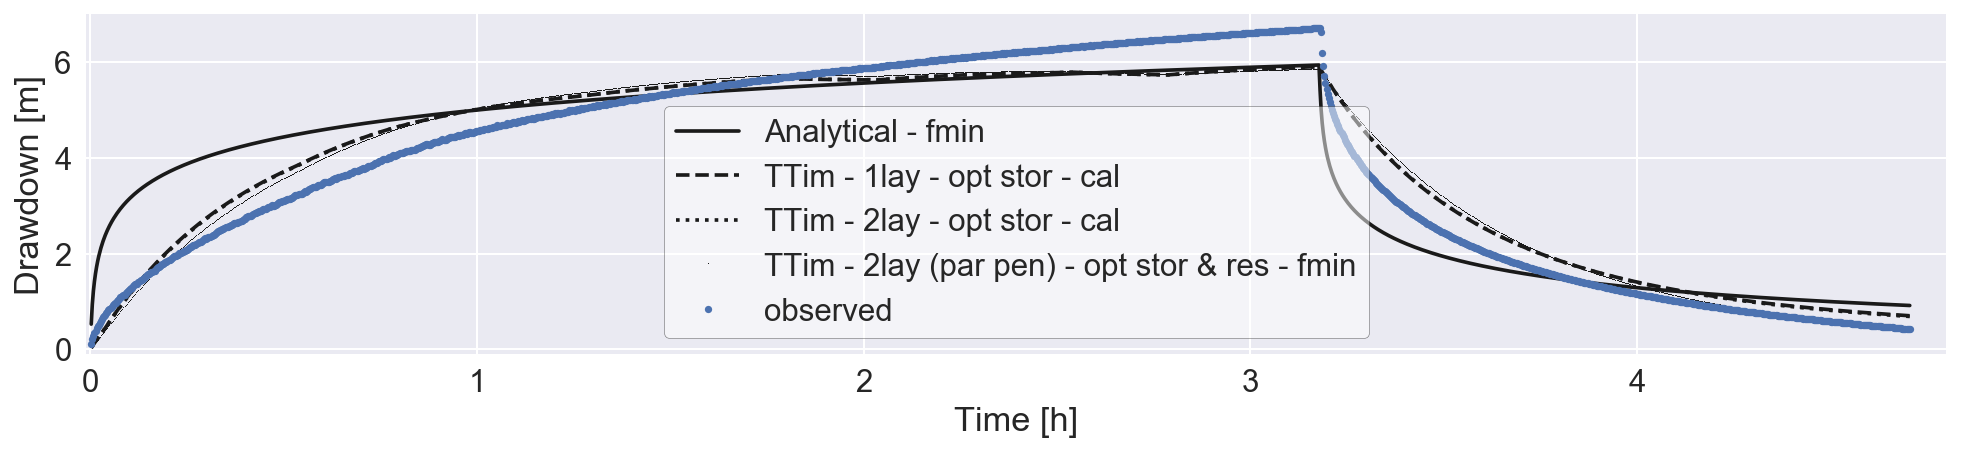
\includegraphics[width=\linewidth]{Nyong_Nayili_multi_lay_best}
 \captionsetup{justification=centering} 
 \caption{Nyong Nayili - Simplified models best fit}
 \label{fig:Nyong_Nayili_best}
\end{figure}

\textbf{Substantive remark} \\
Deviations in obtained data-set and the different (TTim) modelled optimal simulations are of equal size, regardless the optimization function applied. An increase in parameter freedom does not necessarily improve model performance. Reverse effects do occur. In all model simulations the Root-Mean-Square-Error is substantial. The accuracy of the found optimal parameter values can therefore be doubted. Further research on the impact of missing starting data and/or the impact of water inflow during a pumping test is advised.  

\subsection{Location: Janga (1/2)}

\textbf{Site inspection} \\
The infiltration technology near Janga is potentially located at the bank (edge) of a dry river bed. The Volta river is located at walking distance (see fact-sheet visualisation, Appendix \ref{section:fieldworkresults}). A stagnant pond is present at a distance of approximately 70 m from the well. Wet season flooding is caused by river overflow. The flooding is labelled as constant, extreme (>4m) and lasts for months. During field visit no agricultural field is encountered related to the infiltration technology. The pipe segment above surface level accommodates perforations and is equipped with a plastic/concrete cover. \\ 

\textbf{Measurement quality} \\
Bush fires are abundant in the region. Due to close range appearance the test is aborted just before sunset. The duration of recovery process monitoring is affected. Noteworthy is the color change in water discharged during the pumping test. Alternately the water switched color (brownish, grey, white, clear) several times. No further complications occurred. The gathered data can potentially be of use for analysis. \\

\textbf{Fit analysis} \\
Found parameter order size is in line with the data gathered at the other research locations. This does not apply for the Root-Mean-Square-Error scale size. Large RMSE-values can be attributed to the pumping test drawdown part. Shape of the time series is most definitely worth-mentioning. Regardless which method and/or model applied, not a single combination is capable of approaching the remarkable drawdown shape. Analytical Theis method as well as TTim is not capable of correction for irregular patterns of groundwater tables over time. \\

\begin{table}[h!]
\small
\centering
\caption{Janga first attempt - overview best fit parameters}
\label{tab:Janga1_table}
\begin{tabular}{l|c|r|r|rr|rr|c}
\hline 
\textbf{}       & \textbf{Method} & \textbf{Stor [m]} & \textbf{Res [d]} & \textbf{T1}  & \textbf{T2   [m$^2$/d]}  & \textbf{S1}  & \textbf{S2 [-]}  & \textbf{RMSE [m]} \\ \hline \hline
Analytical                & fmin             & -             & -            & 8.84       & -          & 3.0e-01    & -          & 1.339 \\
1 lay                     & fmin             & 0.0635        & -9.7e-03     & 9.09       & -          & 1.6e-02    & -          & 1.382 \\
2 lay                     & fmin             & 0.1287        & -            & 12.48      & 1.3e-04    & 1.9e-02    & 1.1e-08    & 1.445 \\
2 lay (pp)                & fmin             & 0.0635        & -            & 9.1e-05    & 15.19      & 4.3e-08    & 3.1e-03    & 1.530 \\ \hline    
\end{tabular}
\end{table}

\begin{figure}[h!]
 \centering
 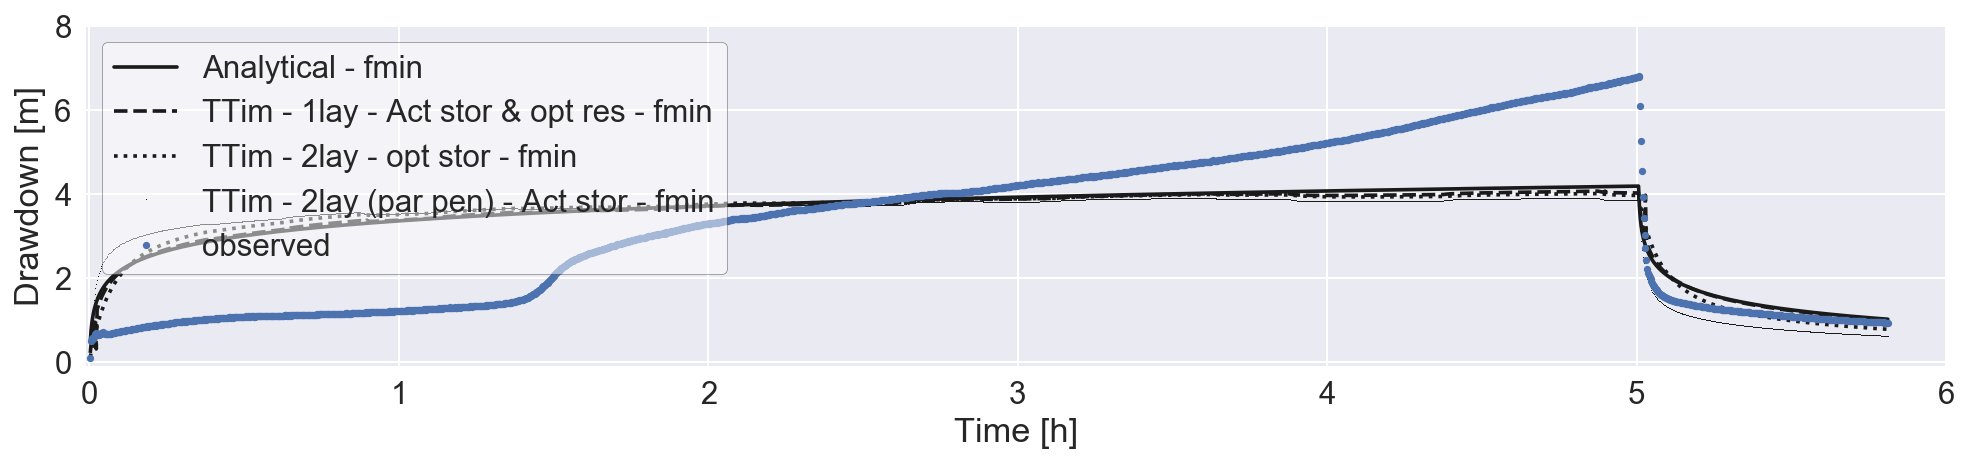
\includegraphics[width=\linewidth]{Janga1_multi_lay_best}
 \captionsetup{justification=centering} 
 \caption{Janga first attempt - Simplified models best fit}
 \label{fig:Janga1_best}
\end{figure}

\textbf{Substantive remark} \\
The course of the drawdown curve is most definitely catching the eye. Several details are striking. There is a sudden increase in drawdown after 90 minutes of pumping. Towards the end of pumping period (four to five hours) the curve does not show the characteristic behaviour of movement towards a new equilibrium. And the fluctuations are no longer monitored in the recovery process. As stated by \citet{Kruseman2000}, most of the time there is not a unique theoretical solution for these well-flow problem. Making the identification of the right (theoretical) system more difficult. Additional fieldwork can provide solutions. Validation is applied to confirm or disprove the correctness of the data-set. The same ASR system is exposed to a second pumping test.

\subsection{Location: Janga (2/2)}

\textbf{Measurement quality} \\
Initial (first two hours) pumping test discharge rates vary slightly (Appendix \ref{section:fieldworkresults}). The drawdown curve is potentially affected. Just as in the first attempt, the extracted water changed color several times. Compared to the previous research a longer monitoring of the recovery process is applied. The collected pumping test time series data is presumably useful. \\

\textbf{Fit analysis} \\
Despite the application of a lower rate pumping test (compared to first attempt) the  gathered drawdown data shows similar behaviour. Lower values in Root-Mean-Square-Error can be assigned to the lower general drawdown pursued and the increased duration of recovery monitoring. It does not necessarily mean the obtained parameter values are more reliable. Values as depicted in Table \ref{tab:Janga2_table} are at most useful as a plausible indication. 

\begin{table}[h!]
\small
\centering
\caption{Janga second attempt - overview best fit parameters}
\label{tab:Janga2_table}
\begin{tabular}{l|c|r|r|rr|rr|c}
\hline 
\textbf{}       & \textbf{Method} & \textbf{Stor [m]} & \textbf{Res [d]} & \textbf{T1}  & \textbf{T2   [m$^2$/d]}  & \textbf{S1}  & \textbf{S2 [-]}  & \textbf{RMSE [m]} \\ \hline \hline
Analytical                & fmin             & -             & -            & 15.97      & -          & 3.0e-01    & -          & 0.571 \\
1 lay                     & fmin             & 5.4e-07       & -9.7e-03     & 13.54      & -          & 1.9e-02    & -          & 0.551 \\
2 lay                     & fmin             & 0.2228        & -2.2e-02     & 2.05       & 8.13       & 2.1e-02    & 4.1e-04    & 0.545 \\
2 lay (pp)                & fmin             & 0.2005        & -3.1e-02     & 6.59       & 0.86       & 9.4e-05    & 2.1e-03    & 0.545 \\ \hline    
\end{tabular}
\end{table}

\begin{figure}[h!]
 \centering
 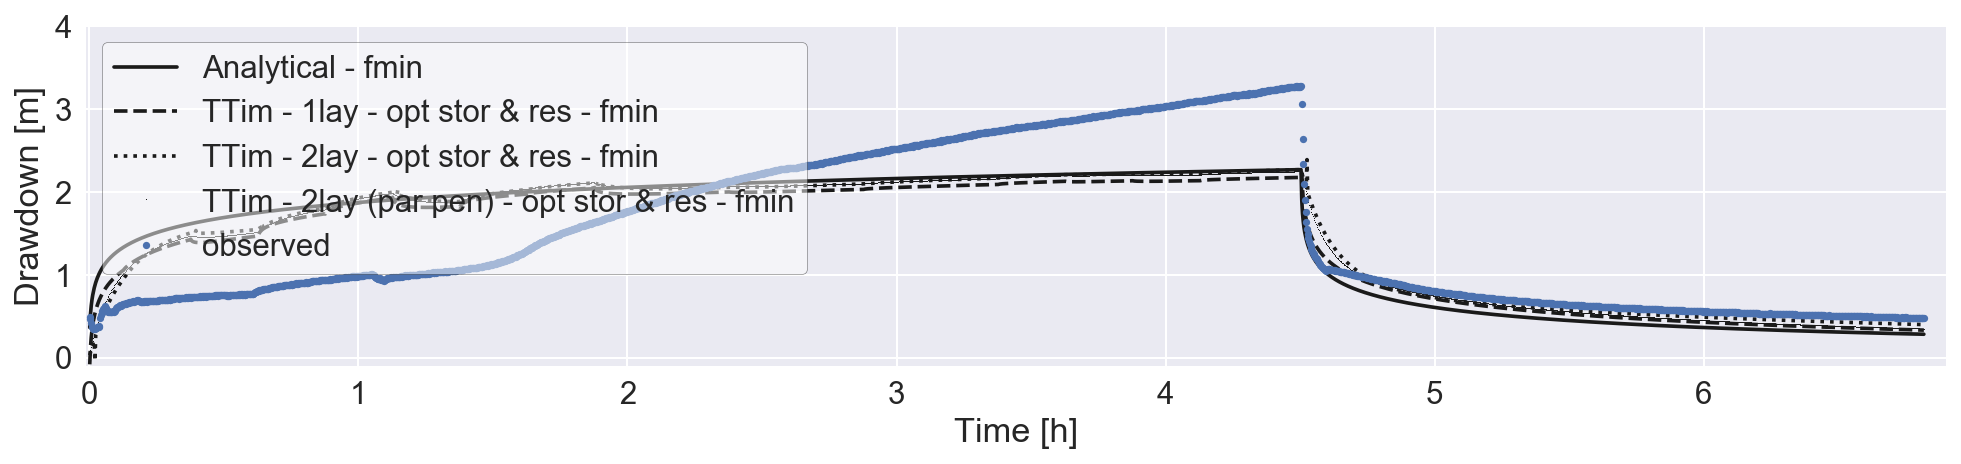
\includegraphics[width=\linewidth]{Janga2_multi_lay_best}
 \captionsetup{justification=centering} 
 \caption{Janga second attempt - Simplified models best fit}
 \label{fig:Janga2_best}
\end{figure}

\textbf{Substantive remark} \\
The applied validation confirms the correctiveness in data gathering. Nevertheless the uncertainty in theoretical model selection persist. A conclusion confirmed by \citet{Kruseman2000}. Causes of the authentic drawdown curve can be widespread. One can think of the drying preferential flow-path  layers, distinctive subsurface connections to the river bed, fracture zones and more. Instead of further fieldwork investigation, it is advisable to gain knowledge in complex drawdwon data interpretation. 

\subsection{Location: Ziong (monitoring)}

\textbf{Site inspection} \\
In the local surroundings of Ziong no river, water flow or ponds are perceived. Wet season land inundation is typically less than 2 m. Day to day variations takes place due to its origin by temporal heavy rain. The regional landscape is flat. Occasionally (bed)rock is observed at the surface. High grasses and bushes are present. Nature is supplemented by several agricultural fields. The infiltration technology does not contain tube perforations above surface level. A steel lid is present to cover the top inlet. Inspection showed the agricultural field related to the ASR-system is ready for the supply of water. \\

\textbf{Measurement quality} \\
During inspection the system was put in daily operation. Instead of a single pumping test, an unique opportunity is seized by an improvised monitoring of the system performance over multiple days. Due to the permanent seasonal pump installation and the limits of diver memory, monitoring divers are positioned in the borehole by an hanging rope only. The inescapable high positioning of the divers (above lowest encountered groundwater tables) results in the absence of multiple time-series segments (yellow dotted line in \ref{fig:Ziong_best}). The adopted discharge rate of 20 m$^3$/d is based on multiple time measurements of the present dated volume meter. In analysis it is assumed to be constant. Operational hours of pumping are not precisely known. In data analysis it is assumed recovery starts four minutes before the first sign of recovery appears in data. Despite these defects the collected data can be used for further analysis. \\

\textbf{Fit analysis} \\
Given the measurements nature no parameter definition is applied by the use of the analytical Theis method. Analysis by the use of TTim show reasonable results. Curve fit simulation shows thorough overlap with the measured time-series. This example shows the wide deployment of TTim. Although above areal prevailing, storativity values are plausible. Obtained transmissivity values are extremely low, but generally consistent. \\

\begin{table}[h!]
\small
\centering
\caption{Ziong - overview best fit parameters}
\label{tab:Ziong_table}
\begin{tabular}{l|c|r|r|rr|rr|c}
\hline 
\textbf{}       & \textbf{Method} & \textbf{Stor [m]} & \textbf{Res [d]} & \textbf{T1}  & \textbf{T2   [m$^2$/d]}  & \textbf{S1}  & \textbf{S2 [-]}  & \textbf{RMSE [m]} \\ \hline \hline
1 lay                     & fmin             & 0.0382        & -            & 1.76      & -         & 1.1e-03    & -          & 0.255 \\
2 lay                     & fmin             & 0.0635        & -0.05        & 0.38      & 1.05      & 2.9e-02    & 1.2e-03    & 0.240 \\
2 lay (pp)                & fmin             & 0.0147        & -0.08        & 0.23      & 0.78      & 2.6e-02    & 1.3e-03    & 0.243 \\ \hline    
\end{tabular}
\end{table}

\begin{figure}[h!]
 \centering
 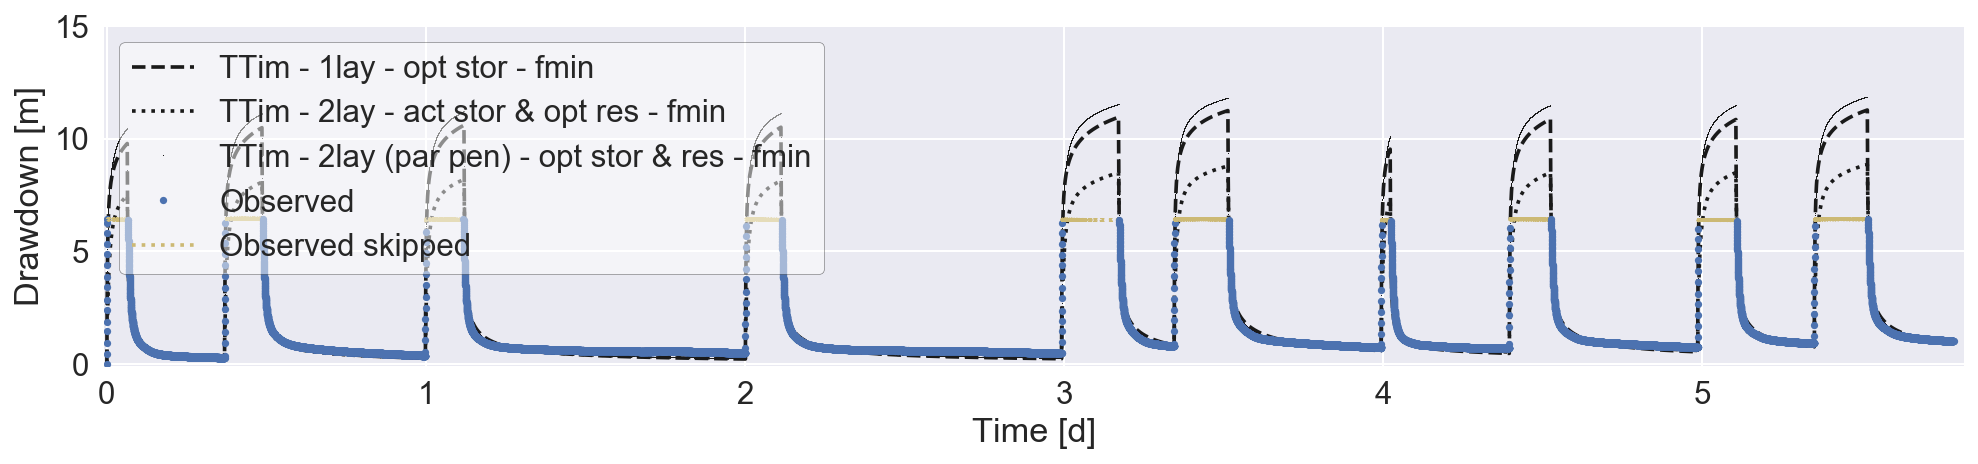
\includegraphics[width=\linewidth]{Ziong_multi_lay_best}
 \captionsetup{justification=centering} 
 \caption{Ziong - Simplified models best fit}
 \label{fig:Ziong_best}
\end{figure}

\textbf{Substantive remark} \\
Both optimization functions (\texttt{Fmin} and \texttt{Calibrate}) can be used for the generation of reasonable parameter outcome. When applying a simplified model with an increased number of degrees of freedom, the \texttt{Fmin} optimization function tends to score slightly better on values for the Root-Mean-Square-Error (Appendix \ref{chapter:Extense_fieldwork_analysis}). This however concerns a single measurement analysis, with a single set of predefined initial parameter. Moreover no other objective functions are taken into account. Regarding the optimisation functions no additional conclusions can be drawn. Looking at the performance of the different simplified models no line of improvement is discovered. Models with an  increased number of degrees of freedom do not necessarily represent nature better. Sometimes reverse effects are even effective. By the use of the right optimal parameter set all three simplified theoretical models are capable to represent the local nature of Ziong to a certain extend. 


%\section{Theoretical validation}
%
%\textbf{Soil analysis}
%
%\textbf{VES analysis}


\section{Results \& conclusions}
\label{section:fieldwork_conclusions}
A brief elaboration on key findings regarding the applied fieldwork pumping tests and data analysis is stated below. The section concludes with parameters definition, applicable on subsequent research. \\

\textbf{ASR-system performance}
\begin{itemize}
\item ASR-system cleaning \\
The ASR-systems of interest are exposed to natural forces. Only one year after construction (2016) the penetration depth of all five boreholes has shrunk. The order of impact differs per location. Most striking example is the borehole at location Nungo. Be aware of the relative fast system degradation. Measures should be taken to prevent the occurrence of clogging. It is advisable to provide each borehole with a plastic/concrete lid. Tube penetrations above the infiltration bed should be sealed permanently to avoid inflow of undesired particles. In addition, annual based preventive cleaning of borehole and infiltration bed is desirable.
         
\item Complementary research \\
Obtained pumping test drawdown data is potentially plausible. Nevertheless, uncertainty in the derivation of parameters and the selection of a (simplified) model consists. As stated by \citet{Kruseman2000}, additional fieldwork does not necessarily solve these uncertainties. No new comparable pumping tests at the same borehole locations are needed at short term. Gaining knowledge on the interpretation of data can possibly offer solutions. Complementary research on how to deal with gabs in pumping test data and/or irregularities in drawdown time-series is advisable. Moreover, future research can be pointed at the impact of (time-dependent) inflow of water during pumping test application. 

\item Future test applications \\
If applied, additional pumping tests should be targeted at the impact of ASR-systems on its surroundings. Pumping tests should be applied in combination with at least one (preferably more) piëzometer at a certain known distance from the well \citep{Kruseman2000}. These tests potentially generate insight in well skin behaviour (degree of resistance). \
The year round installation of one or more divers is an option if complete ASR-system understanding is desirable. This can provides more accurate or new system interpretations. To succeed, it is advisable to set up a measurement plan in advance. Generated data can be used for a more optimal system use.  
\end{itemize}

\textbf{Applicability of methods \& models}
\begin{itemize}
\item Functionality (analytical) methods; Theis \& TTim \\
Compared to the conventional pumping test Theis's method, TTim offers many more model options (borehole storage, well skin resistance, multiple layers) in drawdown data analysis \citep{Mishra2013,Bakker2013}. In this research TTim unsurprisingly outperforms Theis's method. Yet, the attendance of irregular drawdown time-series shows that TTim (e.g. analytical element modelling) also encounters limitations. 

\item Functionality optimization functions; \texttt{Fmin} \& \texttt{Calibrate} \\
Obtained geohyrological parameters represent local nature to a certain extend. This is confirmed by the Root-Mean-Square-Error values (objective function). Application of the two optimization functions generates outcomes. The results of corresponding optimizations can differ in parameter size, but accuracies (RMSE) are comparable (some exceptions). It can be concluded that both optimization functions (\texttt{Fmin} and \texttt{Calibrate}) are potentially usable for the determination of suitable $T$ and $S$ values. 

\item Functionality simplified models  \\
Representation of local nature is pursued by the use of three simplistic system: a single layer system, a double layer system and a system with two layers and partial penetration of the well (Figure \ref{fig:Schematic_1lay_analysis} - \ref{fig:Schematic_3lay_analysis}). Based on the Root-Mean-Square-Error objective function none of these systems sticks out positively or negatively. Therefore, subsequent parts of this research are carried out by the use of the (most simplistic) single layer system. This puts the emphasis on the main goal of this research; effects of ASR-system upscaling.  
\end{itemize}

\textbf{$T$ \& $S$ value definition} \\
Drawdown measurements are performed within the extraction well. A set-up which deviates from the desired common standard \citep{Kruseman2000}. It should be kept in mind the correctness of data can be questioned. From the perspective of robustness two optimization functions (\texttt{Fmin} \& \texttt{Calibrate}) are applied in data analysis. Comparative system optimizations obtain parameters of different size, while Root-Mean-Square-Error values are similar (some exceptions). Moreover, local nature can be represented equally good by a diversity of (single and/or double layered) simplistic systems. For each individual location there is more than one representative parameter-set available. In short, by the analysis of fieldwork data an abundance of uncertainties in parameter definition are present. \\

A bandwidth is defined to deal with these uncertainties. Upper and lower $T$ and $S$ values are stated around the single layer "best" fit solution (Bingo). A visualization of the bandwidth can be found in Figure \ref{fig:Parameter_bandwidth}.   Transmissivity extremes are based on the combination of obtained values in data analysis and a factor of safety. Definition of the outer storativity values needed a different approach. Found values in data analysis more than once approached the predefined boundaries conditions (0 and 0.3 (-)) (Appendix \ref{chapter:Extense_fieldwork_analysis}). These physically improbable parameters are ignored. Outer parameters are preferably based on more common applied values. The chosen lower limit storativity ($S_lower$) corresponds with the situation of a confined aquifer, while the upper limit ($S_upper$) is more related to the specific yield of a phreatic storage (bron: geo1) \citep{Strack1989,Fitts2012}. \\

\begin{figure}[h!]
 \centering
 
\includegraphics[width=0.6\linewidth]{Parameter_bandwidth}
 \captionsetup{justification=centering} 
 \caption{$T$ \& $S$ bandwidth selection}
 \label{fig:Parameter_bandwidth}
\end{figure}

The defined scope can not be interpreted as a generalization of the different locations. Not a single combination of the upper and lower parameter boundaries is the one on one representation of a specific location. The bandwidth predominantly acts as an input for scenario modelling in the subsequent parts of this research. Outcome of these scenarios can only be interpreted as indication of the ASR-system possibilities within northern Ghana. 
\chapter{Model scenarios}
\label{chapter:model_scenarios}
introduction

\section{Model definition}
(representation of whcih nature)

This part of thesis is explorative. Not in correspondece with a single location. 
Hypotetical Northern Ghana situation outlined. Simplistic approach to succeed in the ability of upscaling . used to

aanname van cosntant head 2m verdegingen op basis van interview met locale bevolking 2 m lasting 4 months (entire wetseason) can be possible. 

aanname pomp op 30m, aanname etc  
 Deze scenarios kennen soms echter alsnog vaste aannames. De invloe hiervan zal worden bepaald middels sensitivity analysis. 

\subsection{Research time frame} 
4 months rainfall
8 months dry pumping

\subsection{Soil scenarios} 
explanation by image, ztop, zbot. unconfined, Sy, anistroy

\subsection{Well dimension \& daiy pump schedule}

\section{Modflow model construction}

\subsection{Modflow NWT} (mogelijk als intermezzo)

explanation about model dimension.. Appendix..
explanation about radial conversion.. Appendix
\textbf{layer and column precision}

\textbf{Scale of time}  

\textbf{Well definition}
size, depth, penetrations, 

\textbf{model built elements}
upw applied instead of lpf (gangbaar bij mf2005)
nwt instead of pcg (gangbaar bij mf2005)

\subsection{Modflow MNW2}

\textbf{parameter application} 
1 voor 1 uitleg omtrent de toegepaste parameters. 
Vertel hier ook over de gelimiteerde $Q_des$ middels $Q_thiem$.  

\subsection{Assumptions}

skin factor.. detailed explanation of use!

by the use of MNW2 there is more then multiple nodel connections invilved. This requires the introductuion of well resistance. NOne type not allowed. show equation and where the different components stand for. The A term no longer required. Is a scaling factor between well surface and cell service. Somethioing I did allraeady in my radial scaling. Moreover if the A factor would be applied. rw should be smaller than the representative ro value. This value is about 0.14m. System upscaling (3x initital diameter already exceeds this number. So model failure occurs. C term neglected in this case. Because of manual implementation of the CWC factor. Handy at the same time. Because the CWC of withdrawel can be equalled with the cond in the constant head infiltration period. 

B factor skin factor (reference USGS manual). Kskin typically smaller than kh. Since I'm only using this term to determine CWC it is even required to define Kskin smaller than Kh. If not the skin term and CWC term do become negative. Not allowed and model fails running. so Kskin should be scaled on the known Kh. It can be imagined the Kskin in conditions of low permable soil are relative more close to kh than when kh is better. For now assumption made for sc1 and 2 kskin slightly smaller than kh: kskin = 0.02 m/d. Same values applied for the other scenarios. This is highly arbitrairy. Future research should answer to what extent this assumption is correct. Although it is decisive on absolute ingoing and outgoing volumes. Still it is possible to make conclusions on trends due to upscaling. 

If xcan also take kskin values for the scenarios 3, 4 and 5 slightly smaller than the scenario kh values. But than highly unrealistic volumes are expected. Other option is to scale this bvy the use of the transmissivity values for example. kskin = kh * 1/ T for example. Own idea based on nothing. but than kskin values of respectively 0.022 and 0.021 will be used. Almost the same. \\

sc1b1: kskin groter dan kh kan niet. levert negatieve CWC en cond op. model fails
sc1b1: kskin = 0.02: failed to meet solver requirements
sc1b1: kskin = 0.01: Q-thiem (ongeveer 6.5 m3/d) wordt behaald als grens. hmin op -17.3 m (in de soil), hogere Q zou eventueel kunnen. Is een optie
sc1b1: kskin = 1/5 * kh: Q-thiem wordt op de eerste dag eventjes aangetikt. maar vervolgens elke dag niet meer. Mooi om deze te gebruiken denk ik zo.  voor sc1 (en 2 denk) facor van 1/5 toepassen. verhoog ik vervolgens de Q-des dan zie ik in de eerste tijdastapjes dus iets meer onttrekking. maar daarna  (vanaf dag2) alweer de zelfde Q waardes. Oftwel gelimiteerd door de hlim in de well. Mag ik dit zo doen. want Q-thiem is de Q die je moet onttrekken om op zeer lange termijn pompen een je hlim te bereiken. Nu begrens ik die zelf door hier mijn kskin op aan te passen waardoor ik die hlim (in well) nu al na enkele minuten bereik. Maar hoe anders te doen? \\

idee: die kskin aannemen die zorgt voor Q-thiem in eerste tijdstappen van eerste dag, maar in het vervolg worden losgelaten. Let op bij opschaling van diameter gaat je Q-thiem ook veranderen. \\


sc3b1: kskin = 1/5 * kh levert naar mijn mening al een vrij hoge conductance op. Q-thiem (nu ongeveer 171 m3/d, is dat niet wat hoog?). uitkomst toont aan: dat er ongeveer 20m3 per dag uitgehaald kan worden voor 243 dagen (et dat in 4 u pompen per dag. acht ik sterk onrealistisch. (alhoewel, dit is bij een volledig schoon systeem, wat niet het geval is in northern Ghana.. penlen vaak maar zo'n 10m). Desondanks verhoog ik de weerstand (verlaging conductance). daarom nu bij sc 3 voor kskin = 1/10 * kh gekozen. maar dan wordt Q-thiem iig nooit bereikt. \\


sc5b1: first try met kskin = 1/10 * kh. en Q-thiem is nu 652 m3/d, lijkt me wederom erg erg hoog. dus 1/25 * kh aangenomen. totaal niet wetenschappelijk verantwoord. Hoe dit op te lossen? \\


\section{Base model behaviour}

vertel welke base model is toegepast. Vertel vervolgens het process aan de hand van de meerdere head visualisaties en Q plots. (plot daarbij nog even de $Q_thiem$ lijn). 

doe voor 1 van de scenario's iets meer uitleg middels de plaatjes. (denk hier goed over  na, want wil wel plaatje zien met eerst een Q begrenzing en vervolgens (op het eind van dagelijks pompen niet meer!

laat vervolgens voor de 5 scenarios het base model uitkom zien middels een tabelletje met daarin voor de 5 scenarios dus. $Q_in_tot$, $Q_out_tot$ and $R\%$


\section{Upscaling}
waar het uiteindelijk om draait zijn de waardes van $Q_in_tot$, $Q_out_tot$ and $R\%$ tov het base model. So define new test criteria (opschaling tov het origineel/basemodel). iets van S(Q-in-tot)\% = (new/base)*(1/factor).. potentially intresting. Not strictly required. 


\tikzstyle{mybox} = [draw=black, fill=white, very thick,
    rectangle, rounded corners, inner sep=20pt, inner ysep=20pt]
\tikzstyle{title} =[fill=black, text=white]

\subsection{Upscaling by daily pumping time}

\begin{figure}[h]
\centering
\begin{tikzpicture}
\node [mybox] (box){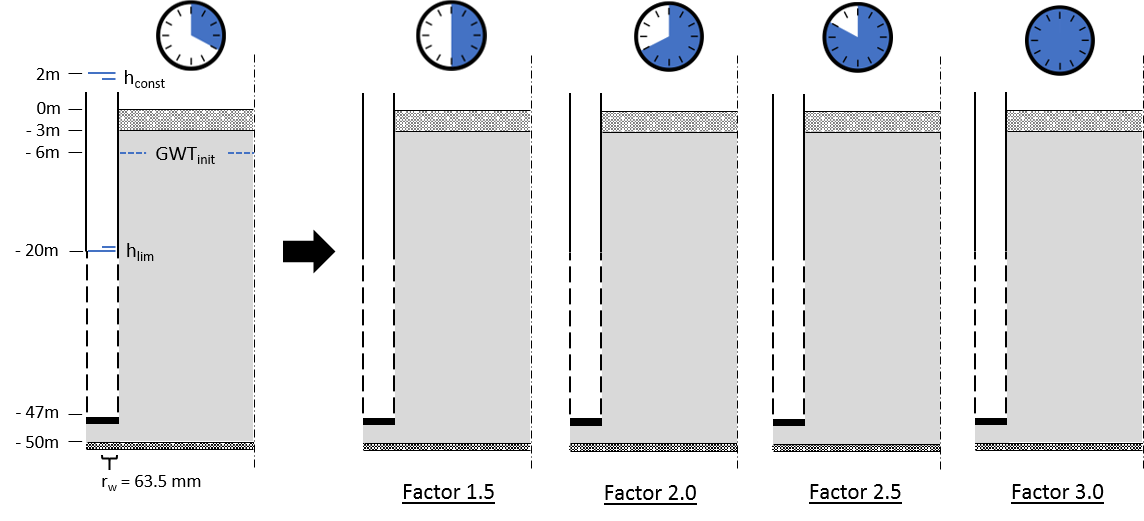
\includegraphics[width=0.9\linewidth]{Schematic_up_time}};  
\node[title, right=10pt] at (box.north west) {Schematic upscaling daily pumping time};
\end{tikzpicture}
\captionsetup{justification=centering}
\caption{Schematic upscaling daily pumping time}
\label{fig:Schematic_up_time}
\end{figure}

\begin{figure}[h!]
 \centering
 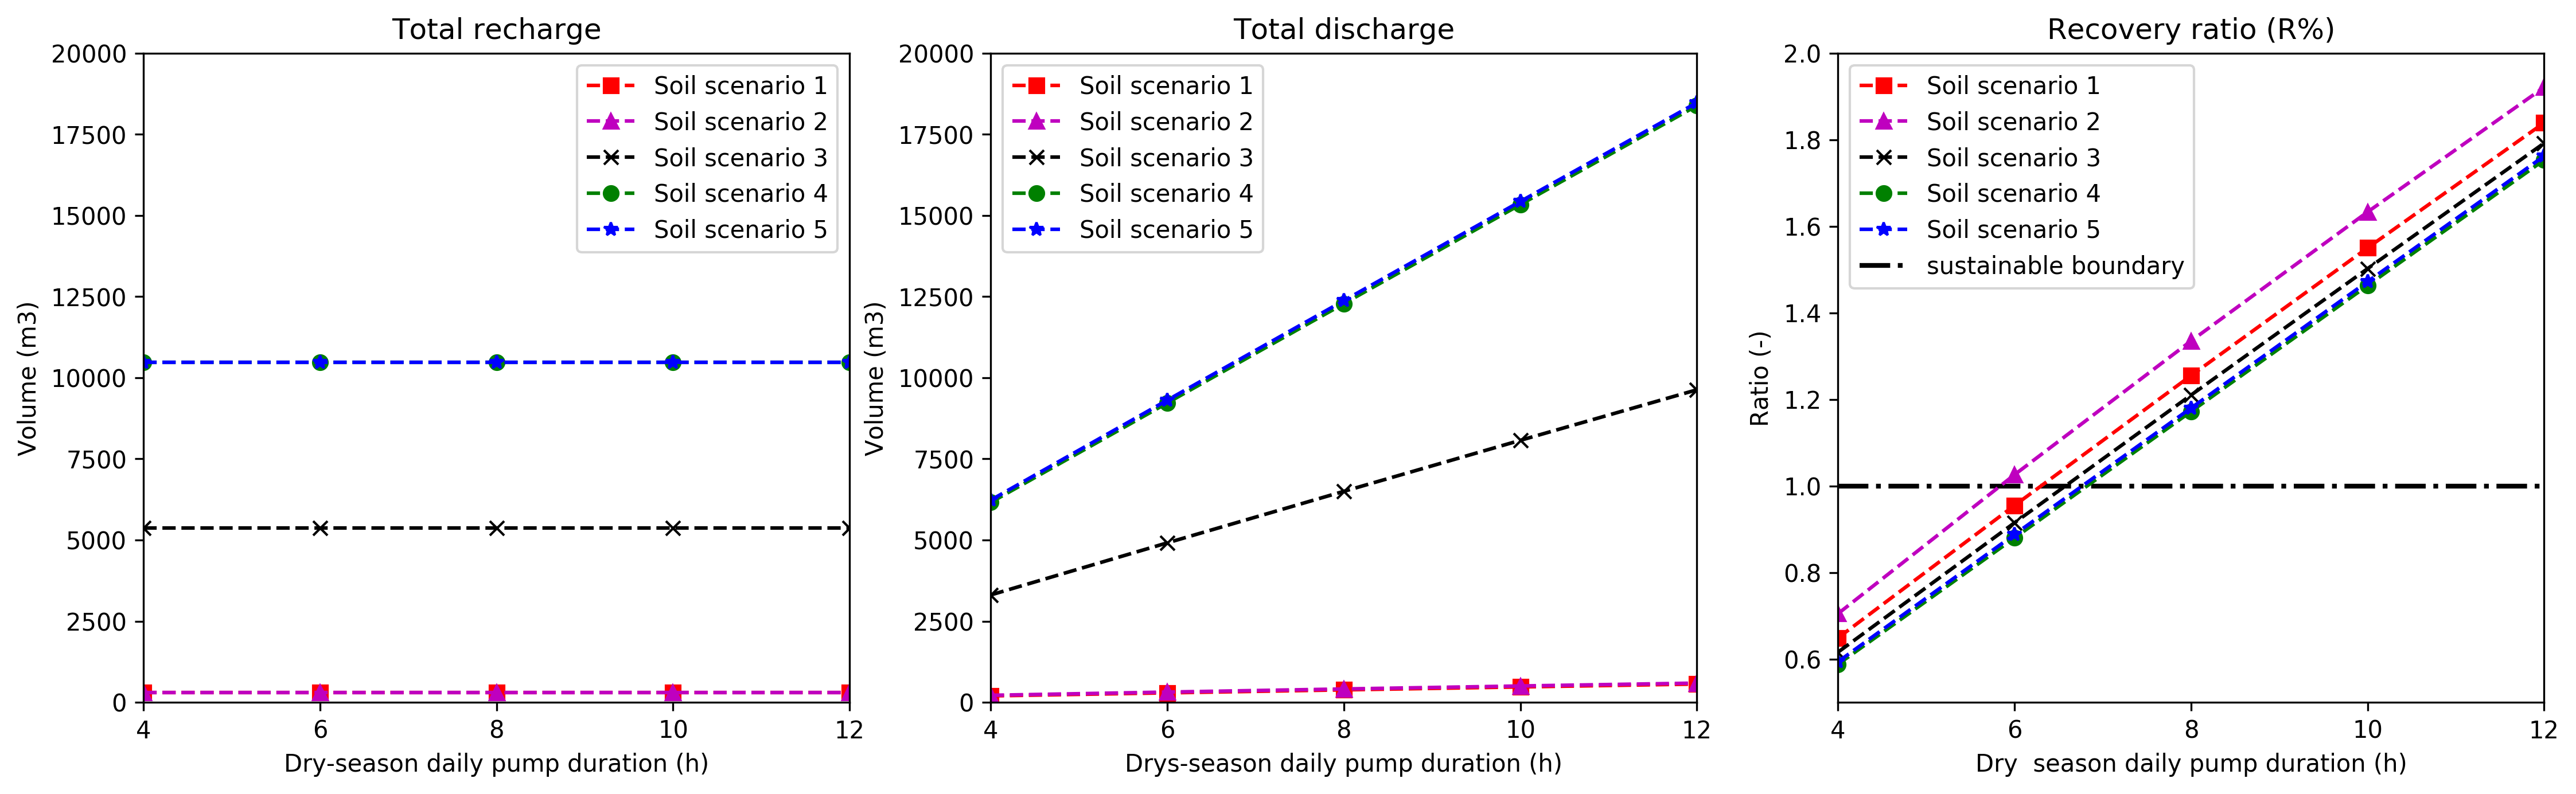
\includegraphics[width=1.0\linewidth]{Results_up_time}
 \captionsetup{justification=centering} 
 \caption{Results of yearly total volumes (in, out, ratio) by upscaling daily pumping time}
 \label{fig:Results_up_time}
\end{figure}

\subsection{Upscaling by borehole diameter}

\begin{figure}[h]
\centering
\begin{tikzpicture}
\node [mybox] (box){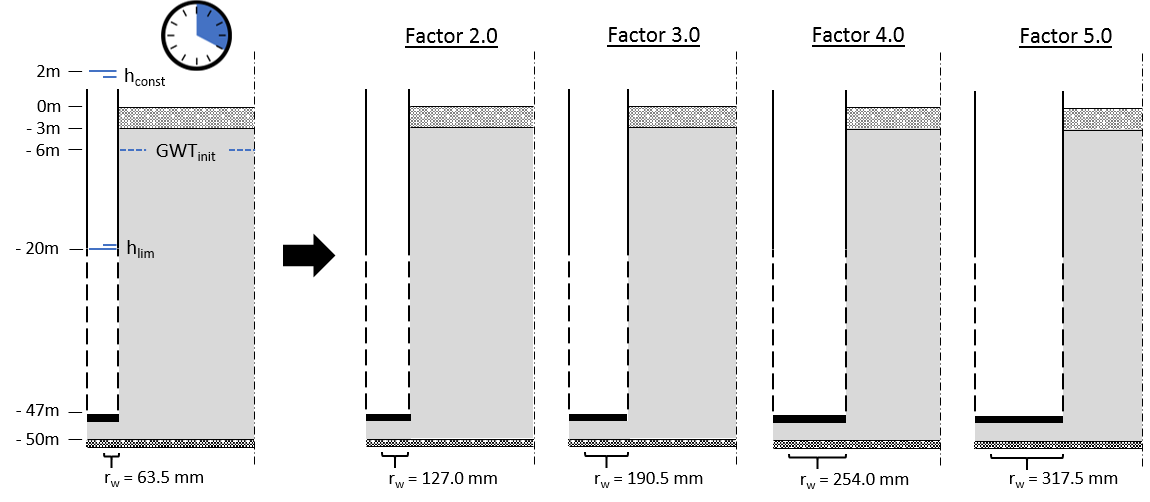
\includegraphics[width=0.9\linewidth]{Schematic_up_diam}};  
\node[title, right=10pt] at (box.north west) {Schematic upscaling well diameter};
\end{tikzpicture}
\captionsetup{justification=centering}
\caption{Schematic upscaling well diameter}
\label{fig:Schematic_up_diam}
\end{figure}

\begin{figure}[h!]
 \centering
 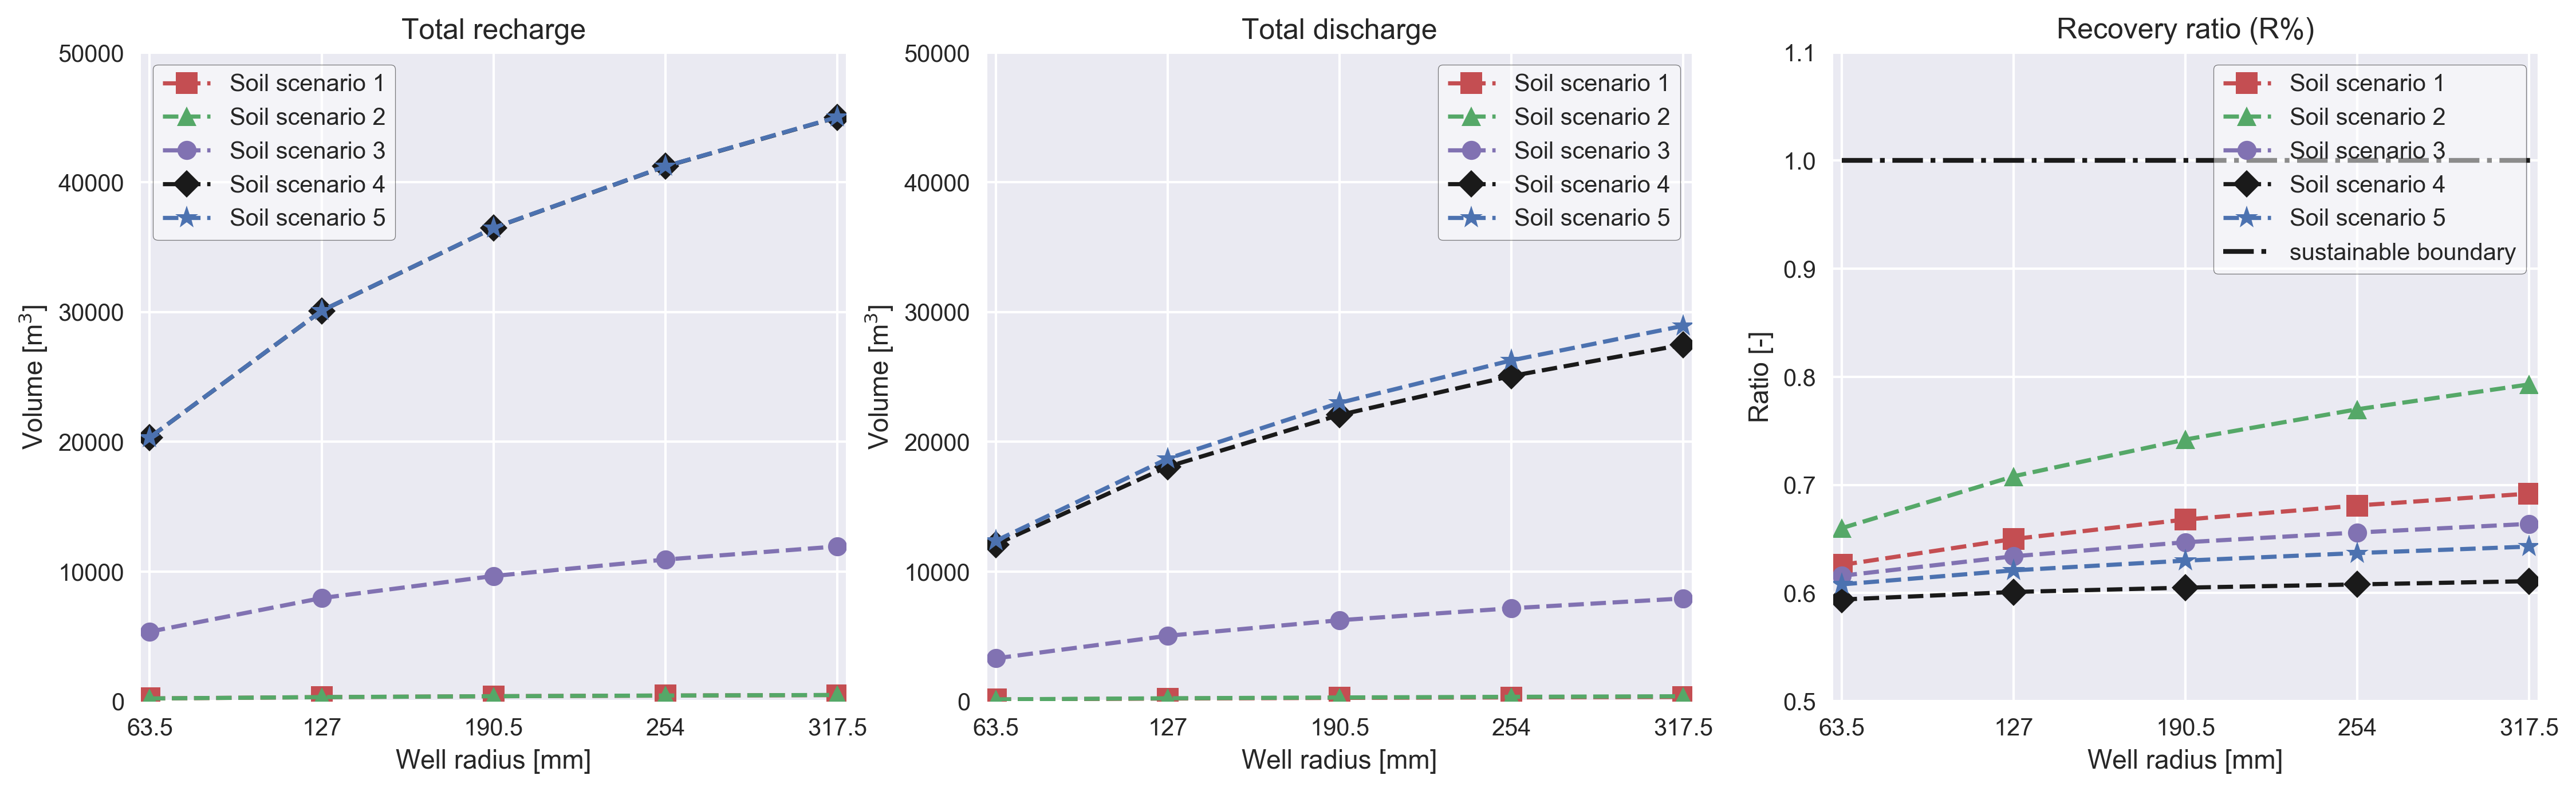
\includegraphics[width=1.0\linewidth]{Results_up_diam}
 \captionsetup{justification=centering} 
 \caption{Results of yearly total volumes (in, out, ratio) by upscaling well diameter}
 \label{fig:Results_up_diam}
\end{figure}


\subsection{Upscaling by cleaning}

\begin{figure}[h]
\centering
\begin{tikzpicture}
\node [mybox] (box){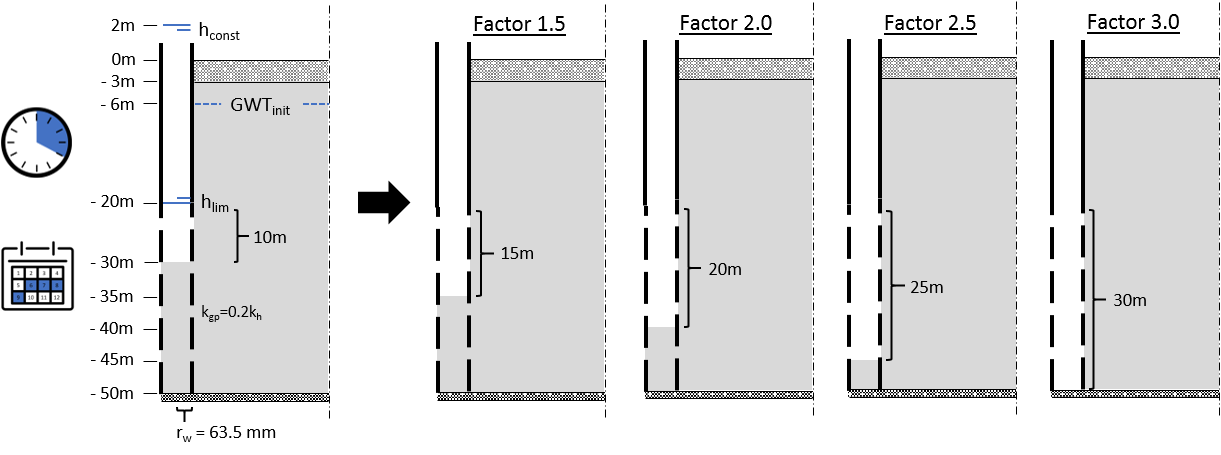
\includegraphics[width=0.9\linewidth]{Schematic_up_clean}};  
\node[title, right=10pt] at (box.north west) {Schematic upscaling well cleaning};
\end{tikzpicture}
\captionsetup{justification=centering}
\caption{Schematic upscaling penetration length due to well cleaning}
\label{fig:Schematic_up_clean}
\end{figure}


\begin{figure}[h!]
 \centering
 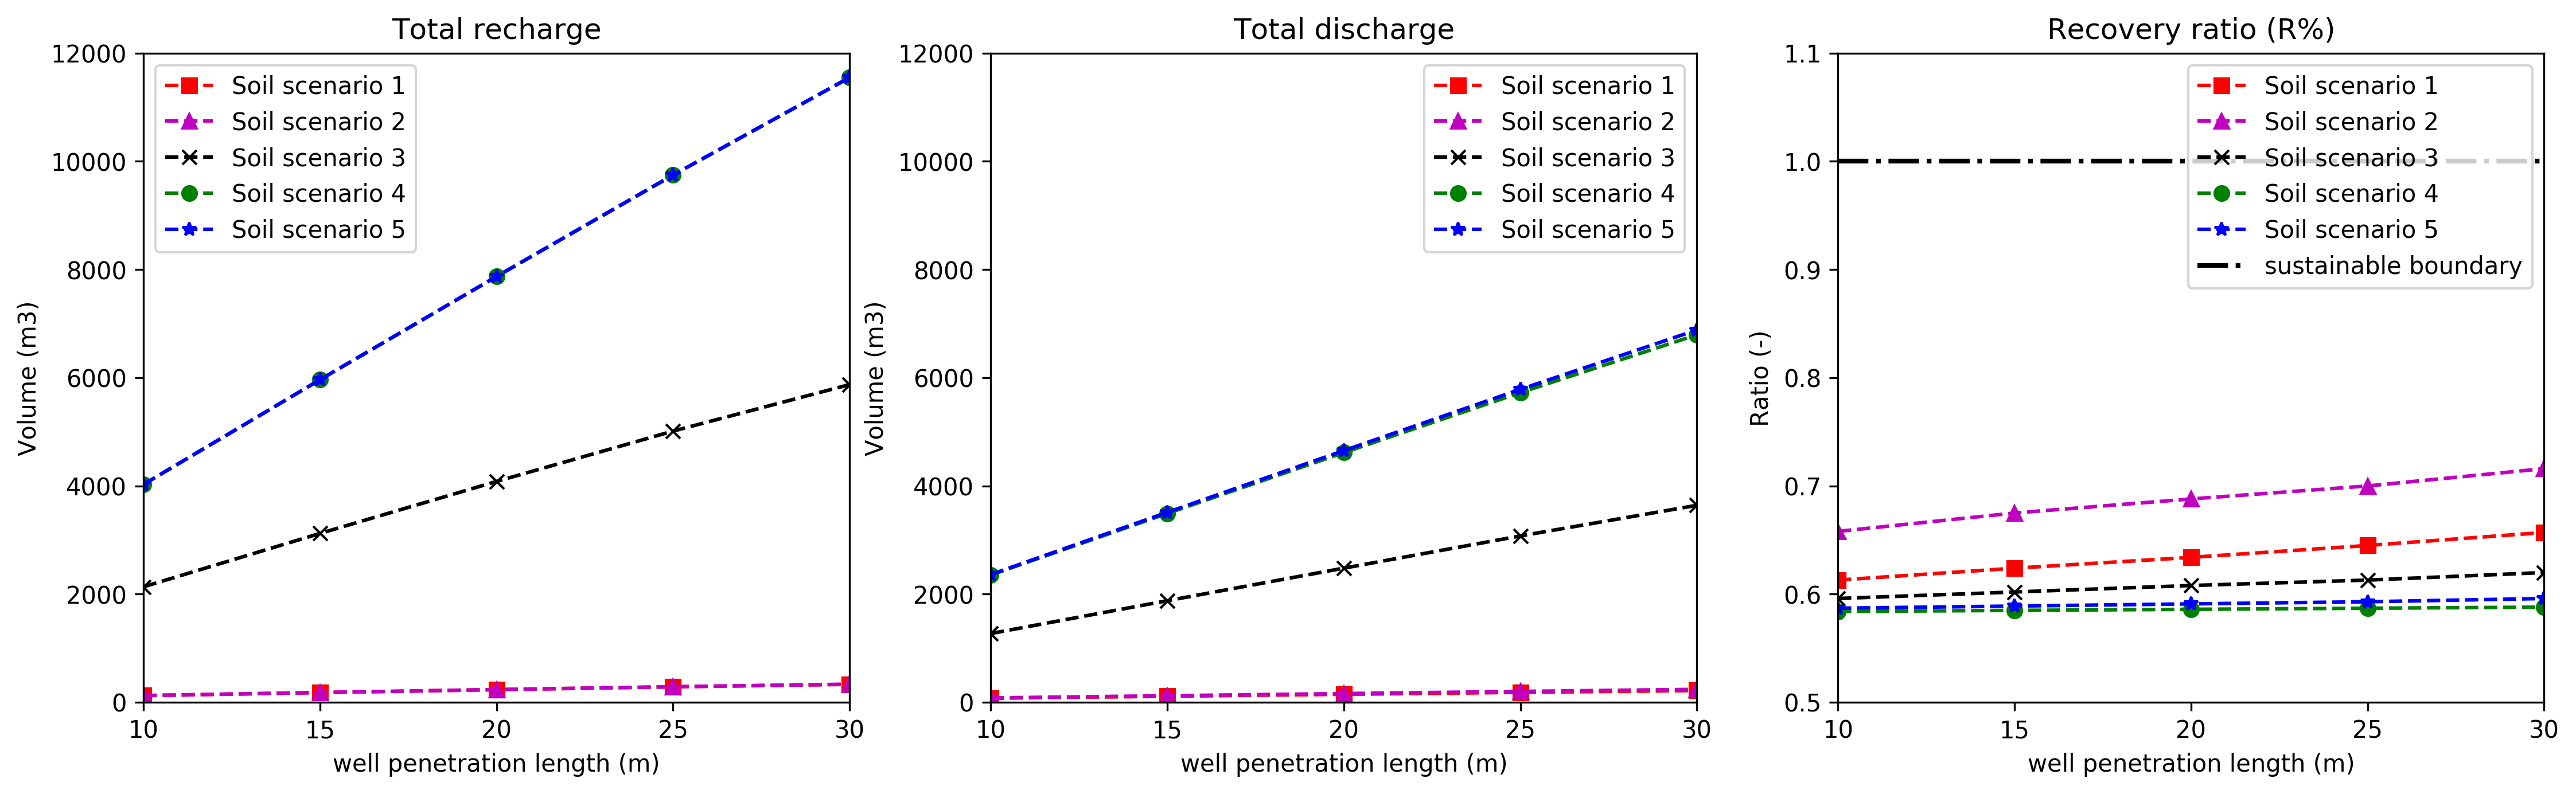
\includegraphics[width=1.0\linewidth]{Results_up_clean}
 \captionsetup{justification=centering} 
 \caption{Results of yearly total volumes (in, out, ratio) by upscaling the penetration length due to well cleaning}
 \label{fig:Results_up_clean}
\end{figure}


\section{Results \& Conclusions}
Korte samenvating dan wel conclusie over de vormen van opschaling. Wat het doet tov de basis. Misschien nog een schaling percentage doorvoeren 
\chapter{ASR system - Business case}
\label{chapter:yield}
The Aquifer Storage and Recovery (ASR) system performances are so far expressed in water volumes. The volumetric results are desirable, but it is hard to get a good picture of it. By the introduction of simplistic rules of thumb, the obtained volumes can be expressed in financial yield. This chapter offers a rough glimpse in the financial feasibility of an ASR system in northern Ghana. \\
The methodology of section \ref{section:Theory_yields} specifies the crops of interest and describes the derivation process of the pumping costs. Section \ref{section:fin_yield} presents the financial yield of respectively the first dry season crop-cycle (tomatoes) and the subsequent crop-cycle (groundnut). In Section \ref{section:pump_costs} the ASR system operational pumping costs are discussed. The agricultural yield is weighted up against the pumping costs in Section \ref{section:Yields_conclusions}. 

%This section contains the conclusions that can be drawn from the site visits and the analysis of pumping test data. The final part of this section describes how this data was used to derive parameters for scenarios to study potential methods for improvements of ASR systems in northern Ghana.   \\

%\section{Methods - ASR system financial yield}
\section{Methods - From water volume to financial considerations}
\label{section:Theory_yields}
This research methodology contains the required information to make a simplistic financial balance on an operational ASR system. The section is split in two. On the one hand, the section presents yield  information. Components as the crops of interest, the irrigation efficiency and the applied exchange rate are addressed. On the other hand, the operation costs are defined. The process from power consumption, due to water withdrawal, to the determination of fuel costs is specified.

% by the definition of system yield versus costs
%with respect to a potential northern Ghana ASR system.
%in a yield and costs section. be subdevided in a yicontains background information on the considered elements of the financial balance. 
% information on considers the 
%The performances of Aquifer Storage and Recovery systems (ASR-systems) are generally expressed in water volumes. The volumetric results are desirable, but it is hard to get a good picture of it. Some simplistic transformations make it possible to express the obtained volumes in agricultural and financial yield.  This part of the methodology facilitates a glimpse in the northern Ghana ASR system (financial) feasibility. The system yield is expressed by the definition of specific crops of interest. The yield is weighted against the water withdrawal pumping costs.
%%An rough insight is given by weighing (crop specfitc First, an explanation on applied theories in transition from water volumes to agricultural field-sizes and financial yields (Section \ref{section:Theory_yields}). Subsequently the previously obtained water volumes are exposed to the transformation (Section \ref{section:Data_processing}). This part of research ends with a conclusive remark on ASR-system yields and posibilities in spatial multiplication (Section \ref{section:Yields_conclusions}). 
%
%(financial and agricultural information) 
% due solely the withdrawal of water,

\subsection{Yield - crops of interest}
\label{subsec:Yield_crop}
Some crops need more water than others. Some crops thrive better in northern Ghana climate than other. Some crops are financially more beneficial than others. And so, many more elements are decisive in the process of crop type determination. This research is not about crop type decisions. The crops are purely included in the study to gain knowledge on hand-on possibilities in the agricultural use and financial feasibility of an ASR-system in northern Ghana. It is chosen to consider the tomato and groundnut crops.\\
%Keeping northern Ghana applicability in mind a selection of crops is made. 

\textbf{Crops of interest}

\begin{figure}[h!]
	\centering
	\begin{subfigure}[b]{0.35\linewidth}
		\centering
\includegraphics[width=0.75\linewidth]{Tom}
		\captionsetup{justification=centering}		
		\caption{\label{fig:Tom}}
		\end{subfigure}%\hfill
	\begin{subfigure}[b]{0.35\linewidth}
        \centering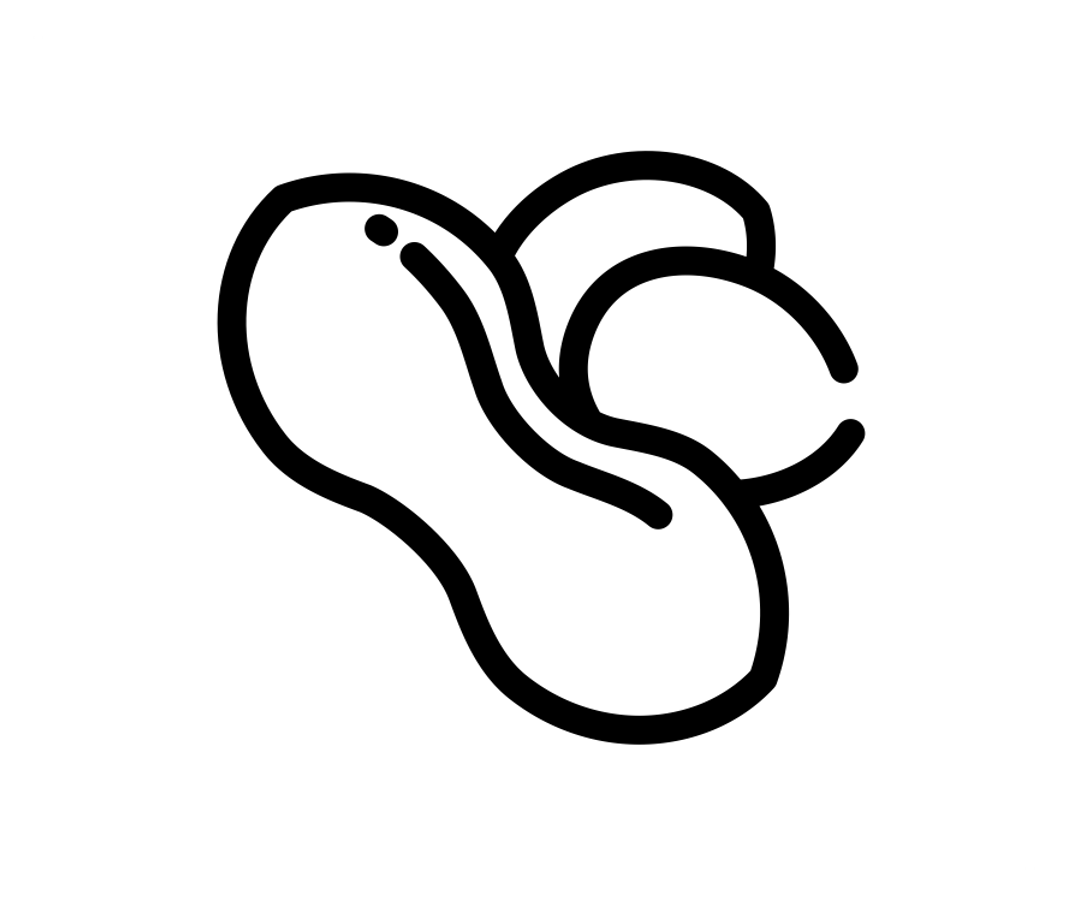
\includegraphics[width=0.75\linewidth]{GN}
		\captionsetup{justification=centering}		
		\caption{\label{fig:GN}}
		\end{subfigure}
		\captionsetup{justification=centering}	
	\caption[Crops of interest: (\subref{fig:Tom}) Tomatoes and (\subref{fig:GN}) Groundnuts]{Crops of interest: (\subref{fig:Tom}) Tomatoes and (\subref{fig:GN}) Groundnuts \\ (visual support by Ben Davis and Lemon Liu from Noun Project - \url{https://thenounproject.com})} 
	\label{fig:Crops}
\end{figure}

\begin{itemize}
\item{Tomato} \\
The worldwide second most important vegetable crop (after the potato) concerns the tomato. Because of its relative high (financial) yield, the vegetable is a desired crop for cultivation. After a period of approximately 90 to 120 days the seeds are grown to fully-fledged crops, the tomatoes are ready for harvesting. Over the growth season the crop thrives best by the supply of 400 to 600 mm of water (rain-fed). To reduce the chances of deceases (pests and infestations) the crop should be cultivated in rotation with other crops. Under the conditions of irrigation the tomato yield is approximately 45 to 65 ton/ha \citep{FAO2018a}. Because of the broad ranges in agricultural yield and water requirements (moreover, only rain-fed statistics), these specific crop competences are not taken into account in research. The derivation of agricultural yield is based on the average 'water utilization efficiency' ($E_y$). For the transformation of agricultural yield to financial benefits, the Esoko march 2018 Ghana average wholesale price is used. The tomato wholesale price is set at a value ranging from 217.86 to 220.43 GHS for a 52 kg crate \citep{ModernGhana2018}. For the purposes of this research the highest average value is applied. To summarize: 
\begin{itemize}
\item{Length growth season: 120 (d)}
\item{Water utilization efficiency: $E_y$ = 11 (kg/m$^3$)}
\item{Wholesale price: 4.239 (GHS/kg)}
\end{itemize}

\item{Groundnut} \\
The groundnut is an above average profitable crop grown in Ghana. Production is often the responsibility of small holder farmers in the North. Almost the complete Ghana groundnut production originates here \citep{Ghana-made2018}. Growth season length is dependent on the varieties (sequential or alternately). In general harvesting can take place after a period of 90 to 140 days. For a proper single season production, groundnut crops require approximately 500 to 700 mm of water. Rain-fed crops can produce average yields of 2-3 ton/ha unshelled nuts. By the introduction of irrigation these values even reach 3.5-4.5 ton/ha \citep{FoodandAgriculturalOrganisationoftheUnitedNationsFAO2018a}.  At the contrary, a 2016 Ghana average agricultural yield of 1.25 ton/ha unshelled groundnut is perceived \citep{FoodandAgriculturalOrganisationoftheUnitedNationsFAO2018}. 
In other words, groundnut crop yield are not unambiguous. The \citet{FoodandAgriculturalOrganisationoftheUnitedNationsFAO2018a} average water utilization efficiency ($E_y$) is adapted as normative. Financial yield highly fluctuates over time. Market forces are dominant in actual returns. The march Esoko 2018 Ghana average unshelled groundnut wholesale price is set at a value ranging from 247.50 to 282.50 GHS for a 82 kg bag \citep{ModernGhana2018}. For the purposes of this research the highest average value is applied and interpreted as the unshelled groundnut price. To summarize:
\begin{itemize}
\item{Length growth season: 123 (d)}
\item{Water utilization efficiency: $E_y$ = 0.7 (kg/m$^3$)}
\item{Wholesale price: 3.445 (GHS/kg)}
\end{itemize} 
\end{itemize}

As stated before, the time frame of the synthetic simulation consist of 243 days of dry season. It is assumed two consecutive growth seasons fit this period. The tomato growth season is succeeded by a growth season labelled for the production of groundnut. This approach is in line with the desire of rotational crop cultivation. \\

The applied crop specifications are dominated by supreme rough assumptions in e.g. quantity (kg) and prices. The obtained (financial) yields should solely be interpreted as indicative. In other words, "All rights reserved". \\
 
\textbf{Irrigation efficiency} \\
The dry season agriculture is assumed to be purely dependent on irrigation for the supply of water. Different types of irrigation are suitable in northern Ghana. One can think of border strip/furrow irrigation; simplistic but inefficient. Higher degrees of efficiency can be achieved by the use of sprinkler irrigation. In the particular case of ASR-system use, minimum water losses are pursued. Therefore, drip irrigation is applied. Drip irrigation is the type of irrigation with the highest efficiencies. The ASR systems are standard paired with facilities as poly-tank(s), pipes and drip hoses. Distances between extraction and irrigation are small, resulting in limited losses. However, water losses are present due to pipe connections and potential evaporation. All-encompassing, a irrigation system efficiency of 0.8 (-) is considered. 80\% of all water withdrawn is assumed to be net usable for crop growth \citep{VandeGiesen2013}. Note, this efficiency number also accounts for the in practice required schedule in irrigation water amounts. Over the growth season the required water volumes are here  hypothetical and assumed to be daily equal. \\
%
%\textbf{Cover area (crop specific)} \\
%Water volumes obtained in previous research sections are basic input for the determination of agricultural field sizes. Net withdrawn (dry season) total volumes are divided by the crop specific water footprint. The areal outcome is halved to correct for the double (consecutive) growth periods in a single dry season.   
%
%\begin{equation}
% A = \frac{V_{out,tot} * \eta_{irrigation}}{2 * Water footprint_{crop}} 
%\label{eq:A}
%\end{equation}
%
%Where, A (m$^2$) is the agricultural field area, $V_{out,tot}$ (m$^3$) is the dry season total volume discharged, $\eta_{irrigation}$ (-) is the irrigation efficiency and $Water footprint_{crop}$ (m) is the crop specific water footprint. \\
%
%The extraction of water leaves marks on nature. Pump operation causes a groundwater cone of depression. Close range (and most definitely in-well) drawdown is significant. At an increased radial distance impact losses magnitude. For system spatial multiplication it is of interest to define a maximum circular area in-which groundwater is affected. The groundwater cone of influence (G) is defined as the area corresponding with the maximum radius from well at which the groundwater drawdown is labelled as significant. In this study, significance is assumed to be bounded by a drawdown of 1.0 m at any moment in year. \\
%
%\begin{figure}[h]
% \centering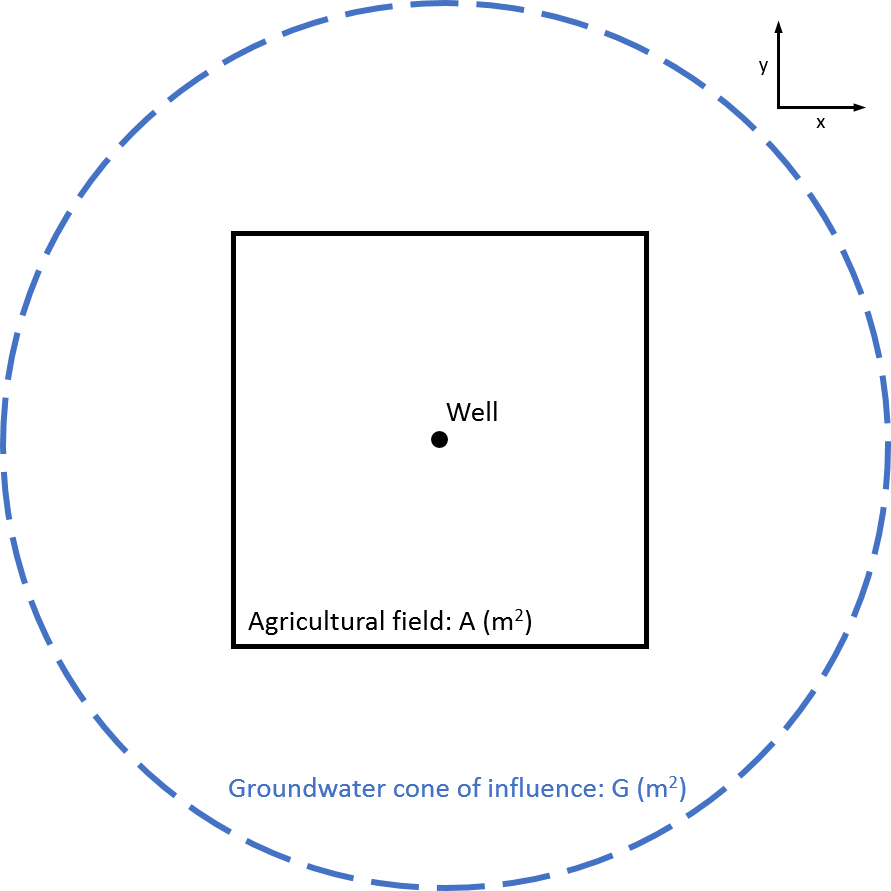
\includegraphics[width=0.4\linewidth]{Crop_cover}
% \captionsetup{justification=centering}
% \caption{Fictive schematic of crop cover area (C$_\%$)}
% \label{fig:Crop_cover}
%\end{figure}
%
%The A over G ratio ($C_{\%}$) shows top-view perspectives of spatially concatenated multiplication of agricultural fields, as visualized in Figure (\ref{fig:Crop_cover}). High $C_{\%}$ values (close to one) suggest the implementation of agricultural fields is possible at close mutual distance. \\
%
%\begin{equation}
% C_{\%} = \frac{A}{G}
%\label{eq:RR}
%\end{equation}
%
%Where  C$_{\%}$ is the crop cover ratio (-), $A$ (m$^2$) is the crop specific agricultural field size and $G$ (m$^2$) is the areal groundwater cone of influence. \\

\textbf{Financial yield} \\
Based on the described crop specification, the simulated water volumes withdrawn can be expressed in financial returns. The agricultural yield (kg/m$^3$) and the weighted crop prices (GHS/kg) are defined. From consistence considerations it is chosen to express the financial returns in US dollars. The July 7$th$ Bloomberg financial exchange rate is applied: 0.2081 USD/GHS \citep{Bloomberg2018}.

\subsection{Costs - water withdrawal}
The ASR system profits are accompanied by costs. For this research all Capital Expenditures(CAPEX) are unknown and ignored. The same applies for large parts of the Operating Expenses (OPEX), e.g. farmer wage and fertilizer costs. The only costs accounted in this research are the costs related to the energy (diesel) consumption due to pumping. Outcomes are purely focused on the feasibility of the daily system operation. An impression is generated, whether or not regular ASR-system operation on its own is profitable. \\

\begin{figure}[h!]
 \centering
 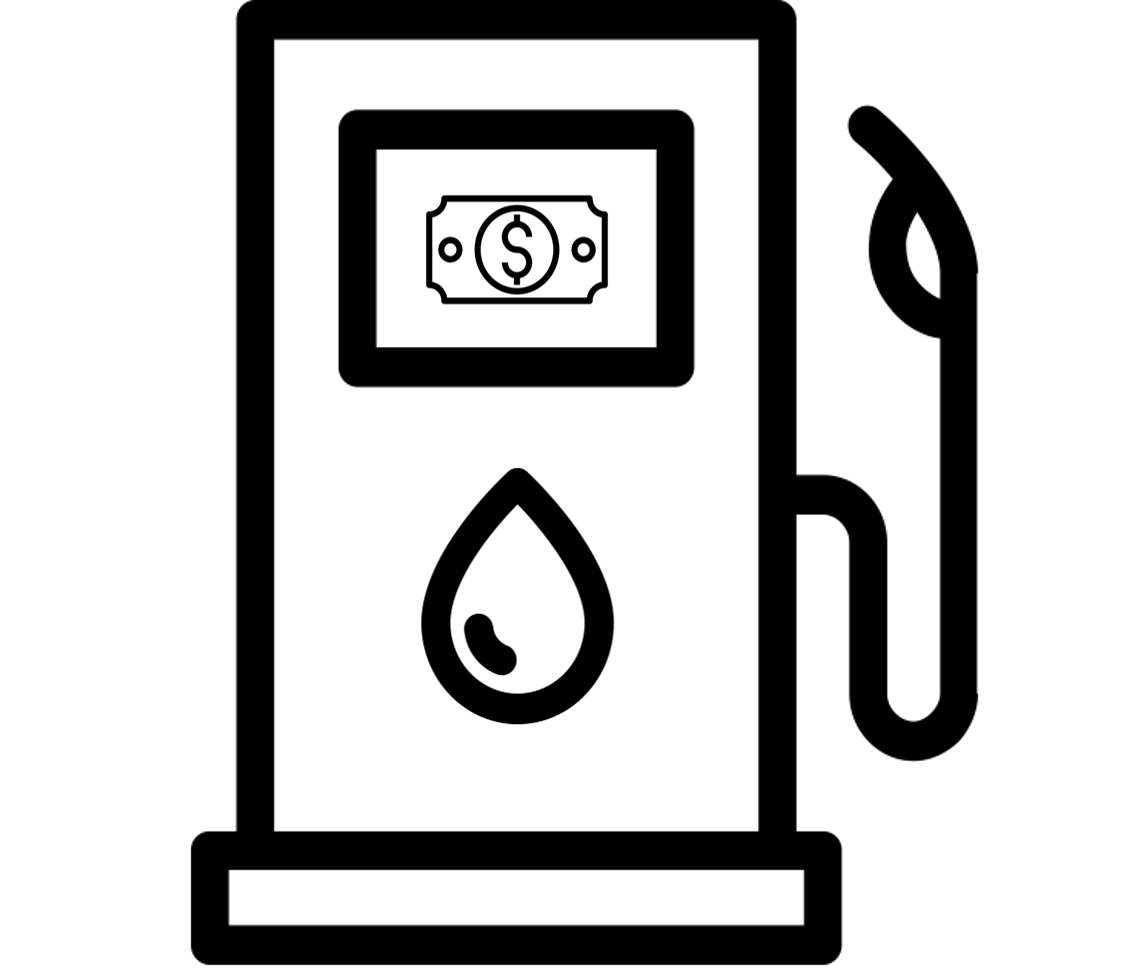
\includegraphics[width=0.35\linewidth]{Schematic_pump_costs}
 \captionsetup{justification=centering} 
 \caption[Schematic of the ASR system operational pumping costs]{Schematic of the ASR system operational pumping costs \\ (visual support by Nociconist, Quan Do and Phonlaphat Throngsriphong from Noun Project - \url{https://thenounproject.com})}
 \label{fig:Schematic_pump_costs}
\end{figure}

\textbf{Synthetic pump application} \\
The Pedrollo 4" submergence pump is applied in fieldwork measurements. The same pump, i.e. its specifications, is used a standard in the subsequent parts of research. General specification can be found in Appendix \ref{chapter:Pedrollo_product_specs}. The results of the synthetic simulations contains time dependent (4 hours daily, 243 days) discharge rates. As soon as the maximum pumping capacity is exceeded (at any moment), it is assumed the specific dry season simulation is carried out by the implementation of (one or more) extra (same) pump(s). By a parallel pump configuration the same heads and efficiencies are ensured, while discharge capacities are multiplied \citep{VandeGiesen2013}. \\ 
%As soon as the maximum pumping capacity is exceeded by the obtained (simulated) discharge rates (results Chapter \ref{chapter:model_scenarios}),

\textbf{Energy Consumption} \\
The available groundwater has to be lifted to the surface. Depends on the obtained discharges, the lifting action requires a certain magnitude of power (Equation \ref{N_net}). For water displacement the difference between pump position and surface level (30m) is retained. An extra lift of 15 m is added to account for friction losses and the higher position (above surface) of the poly tank(s). A total head lift of 45 m is applied.

\begin{equation}
N_{net} =  g * Q * \Delta H
\label{N_net}
\end{equation}

Where $N_{net}$ (kW) is the net power required, g (m/s$^2$) is the gravitational acceleration (9.81 m/s$^2$), Q (m$^3$/s) is the dry season discharge (time dependent (and in seconds)) and $\Delta$H (m) is the net head (total lift) required. In this equation it is assumed the water has a density of 1000 kg/m$^3$. \\

In general, the use of power gets accompanied by losses (for example due to friction and turbulence). Ever single power-related equipment works at a certain level of efficiency. The power generator applied in fieldwork (Appendix \ref{chapter:fieldwork_set-up}) is used over years. Due to its datedness, a generator efficiency of 70\% is estimated. The efficiency of the Pedrollo pump(s) is dependent on the discharge rate during dry season operation. An overview of the efficiency curve is present in Appendix \ref{chapter:Pedrollo_product_specs}. In this study, the pump efficiencies are related to the time dependent discharges obtained in the synthetic model simulations. Besides equipment losses, energy get lost due to mutual transmission. An extra efficiency value of 90\% is accounted \citep{VandeGiesen2013}. Result is a variable ASR system efficiency that never exceeds 36.5 \% (based on the maximum pump efficiency of 58\%).

\begin{equation}
 \eta_{total} =   \eta_{generator} * \eta_{transmission} * \eta_{pump} \end{equation}

Where $\eta_{total}$ (-) is the overall power efficiency, $\eta_{generator}$ (-) is the generator power efficiency, $\eta_{transmission}$ (-) is the transmission power efficiency and $\eta_{pump}$ (-) is the pump power efficiency. \\

The combination of total ASR-system efficiency and net required power results in a gross power (Equation \ref{Eq:gross}). The gross power should be delivered by the generator to gain the desired volumes of water at the agricultural fields. Multiplying the gross power required by the total hours of pump operation returns the total energy consumed (kWh).

\begin{equation}
 N_{gross} =   \frac{N_{net}}{\eta_{total}}
\label{Eq:gross}
\end{equation}

Where $N_{gross}$ (kW) is the gross power required, $N_{net}$ (kW) is the net power required and $\eta_{total}$ (-) is the overall power efficiency. \\

\textbf{Energy costs} \\
The Kipor power generator (Appendix \ref{chapter:fieldwork_set-up}) contains a 15 liter diesel tank. On a fully filled tank the generator can operate for 6.5 hours. A fuel consumption of 2.31 l/h is taken into account. During operation the generator delivers a continuous power capacity of 4.5 kW \citep{TS242018}. The Ghana diesel price of 5.03 GHS/l (begin of July 2018) is adopted as normative \citep{GlobalPetrolPrices2018}. The Bloomberg financial exchange rate (0.2081 USD/GHS) is also applied on the fuel costs for proper financial comparison \citep{Bloomberg2018}.

\begin{equation}
 Cost_{fuel} =  \frac{consump_{gen} * price_{fuel} * rate_{exchange}}{power_{gen}}
\end{equation}

Where $Cost_{fuel}$ (USD/kWh) is the price of fuel,  $consump_{gen}$ (l/h) is the generator fuel consumption,  $price_{fuel}$ (GHS/l) is the fuel price in Ghana, $rate_{exchange}$ (USD/GHS) is the Bloomberg financial currency rate and $power_{gen}$ (kW) is the generator continuous power capacity. \\

\section{Financial yield}
\label{section:fin_yield}
The impact of the different ASR system improvements are (amongst others) expressed in terms of total volumes discharged (Section \ref{subsec:improvements}). These volumes are the summed-up results of eight months daily groundwater withdrawal, where discharge rates are limited due to the set bound in GWT drawdown (14 m). The time dependent discharge volumes of the first four months (120 days) are allocated for the production of tomatoes (one cropping season). The groundwater withdrawal of the subsequent 123 days of dry season is assigned to a single cycle of groundnut cultivation. The corresponding financial yields are acquired by subjecting the obtained water quantities to the volume-to-yield methods (described in Section \ref{subsec:Yield_crop}). The crop-specific financial results are for each soil scenario and for each type of ASR system improvement (multiple steps) presented in Figure \ref{fig:tom_yield} (Tomatoes) and Figure \ref{fig:gn_yield} (Groundnut). \\

The determination of the financial yield is based on highly simplistic methods. The obtained revenues are purely based on a crop-specific factorization of the derived discharge volumes. Therefore, the (improved) ASR system revenue (USD) patterns are in line with the prior presented total discharge volumes (m$^3$). The results show that higher (financial) yield can be expected by the implementation of the explored types of ASR system improvement. Exact revenues are dependent on the type and 'size' of improvement. The financial yield of the synthetic base model (values on the Figures absolute left-side) is utmost somewhat more than doubled by the explored research scope of system improvements. \\

%* The obtained results are all based on volume-to-yield transformations described in Section \ref{section:Theory_yields}. \\
%%\subsection{Financial yield}

 \begin{figure}[h!]
 \centering
 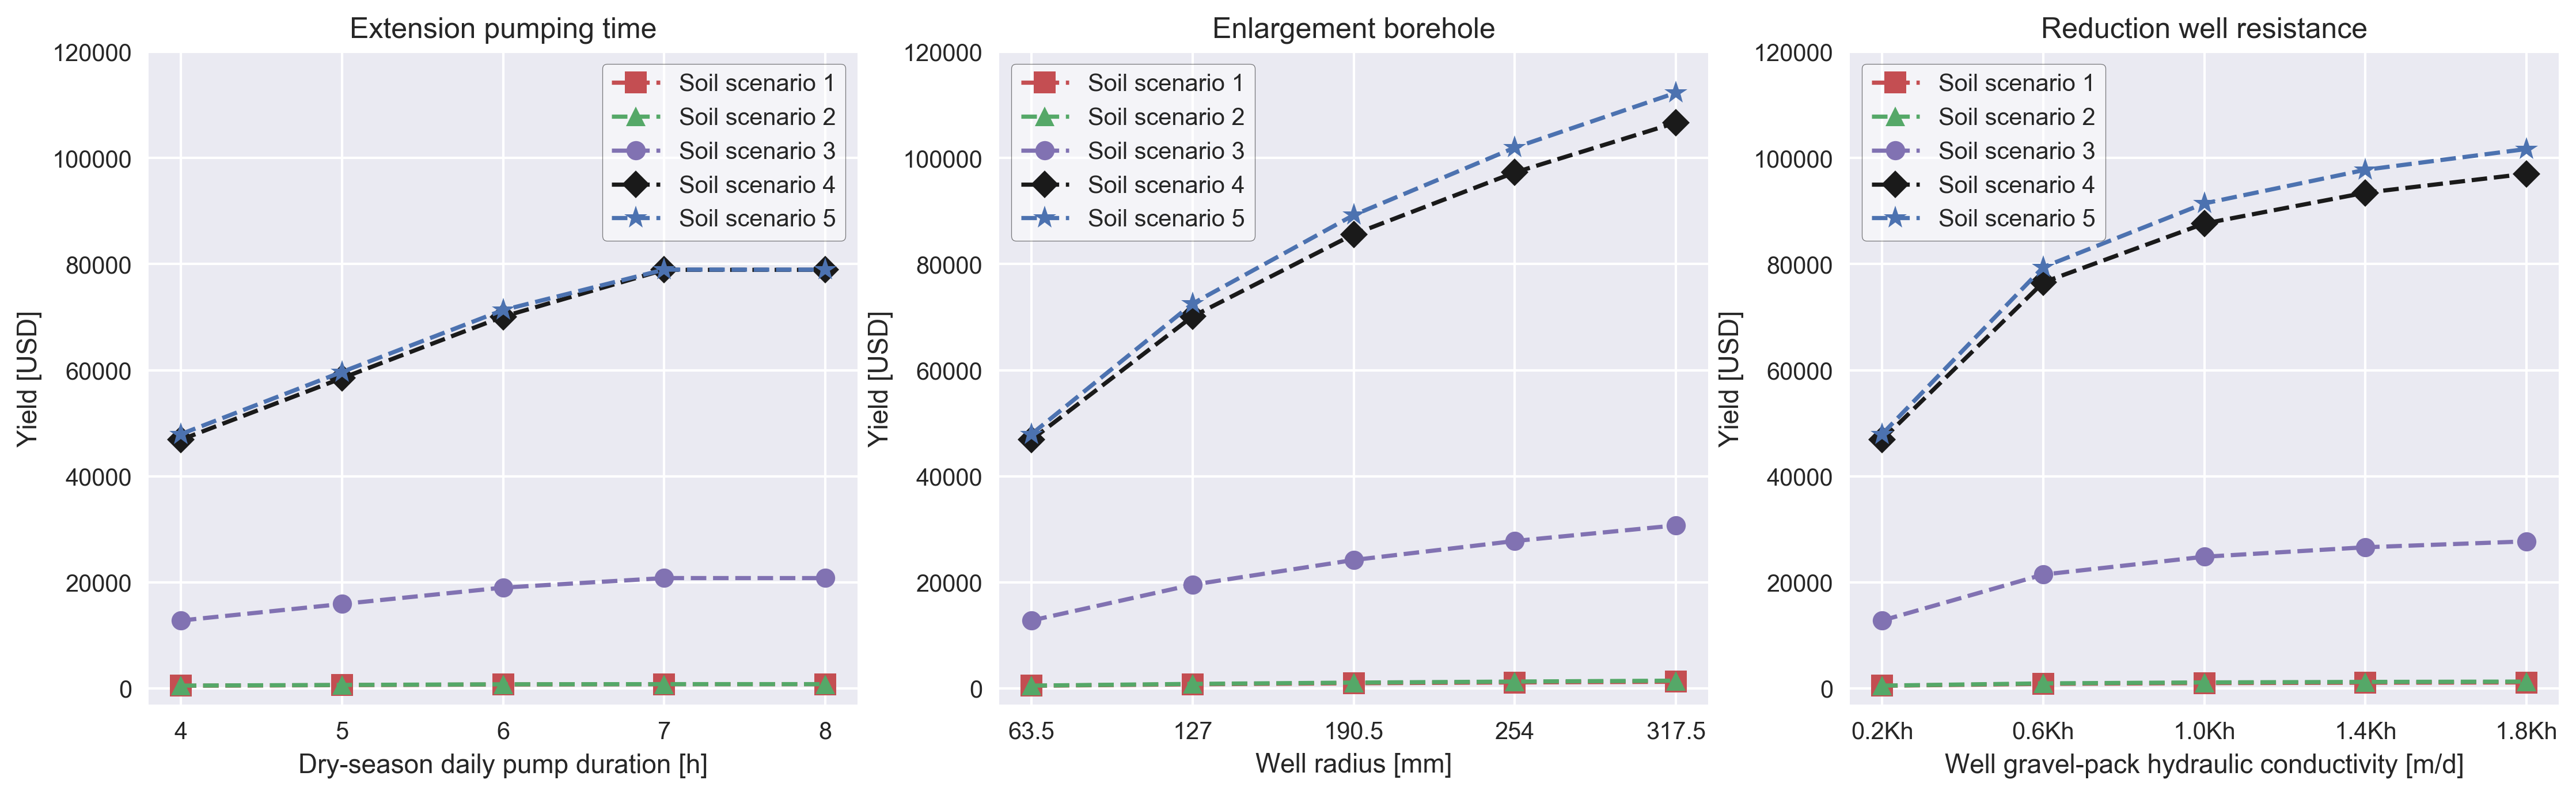
\includegraphics[width=1.0\linewidth]{tom_yield}
 \captionsetup{justification=centering} 
 \caption{Financial yield - Tomatoes (4 months) - three types of ASR system improvement}
 \label{fig:tom_yield}
\end{figure}

\begin{figure}[H]
 \centering
 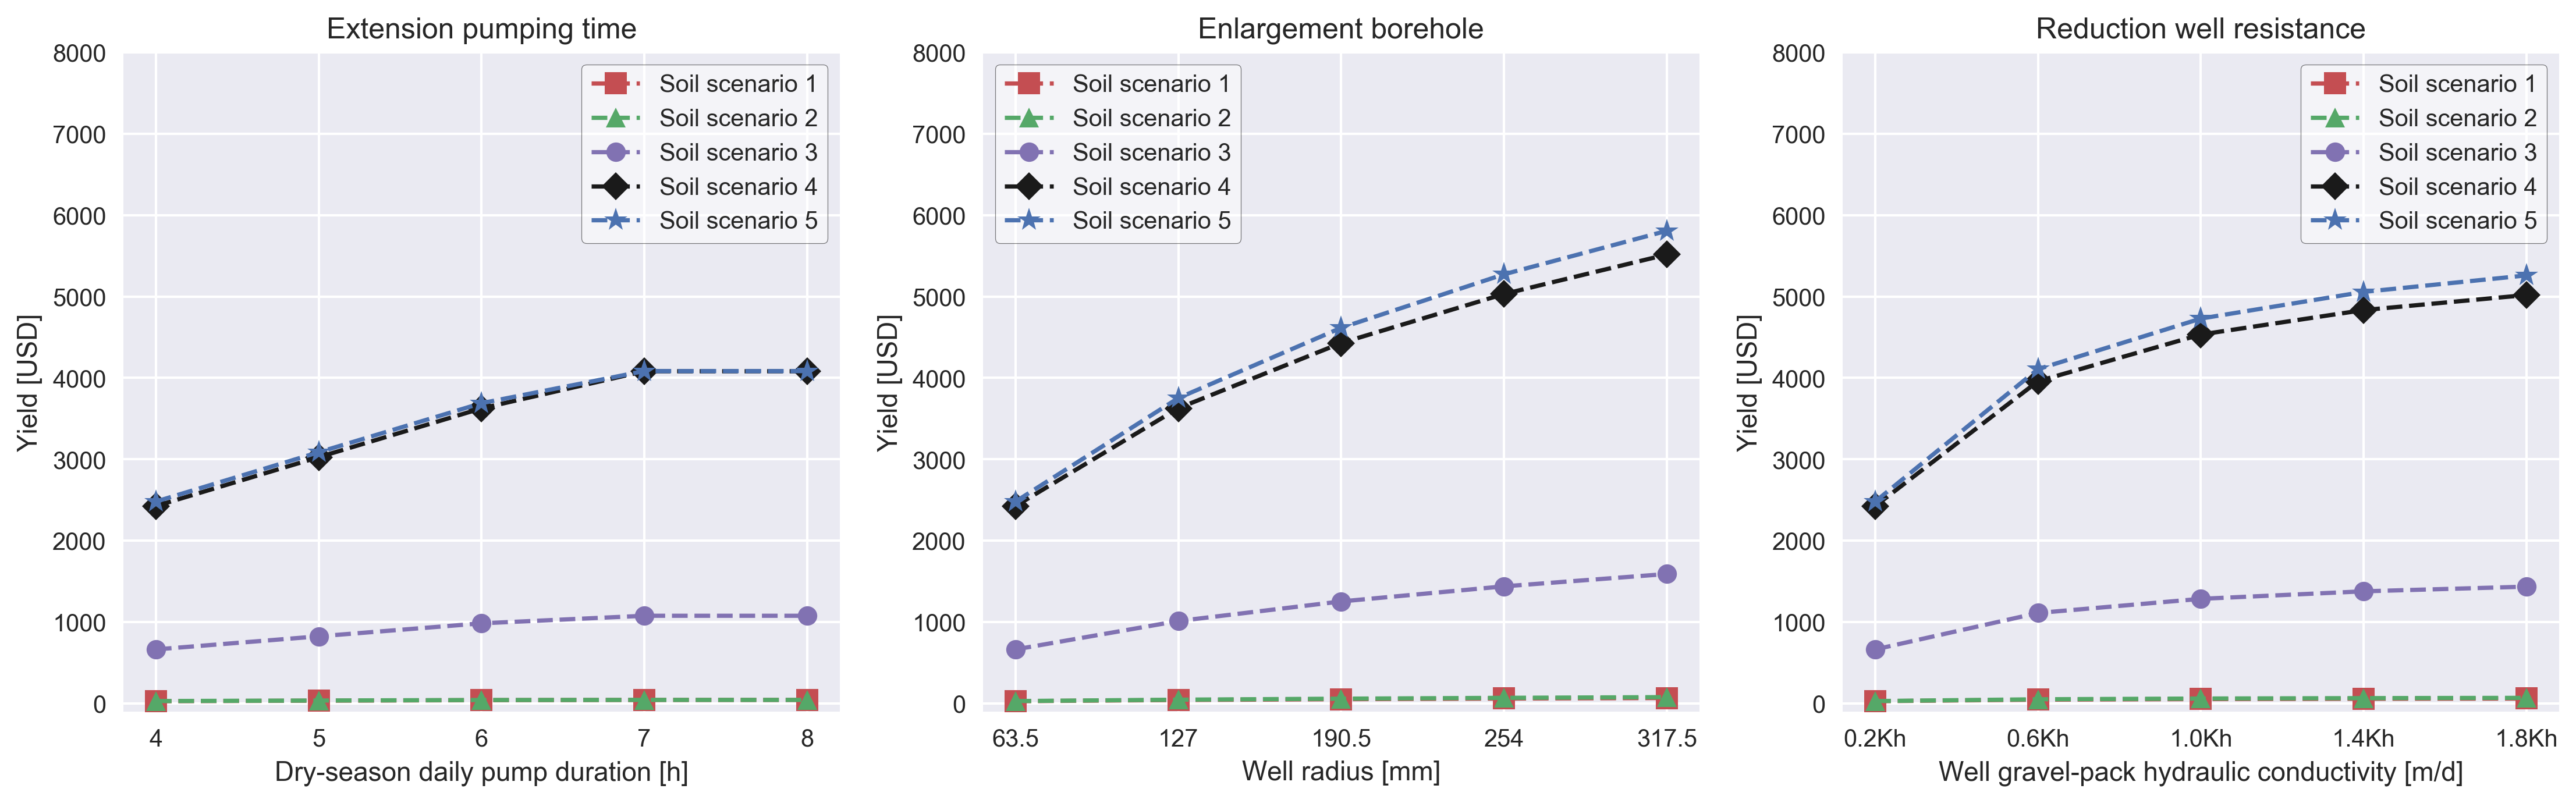
\includegraphics[width=1.0\linewidth]{gn_yield}
 \captionsetup{justification=centering} 
 \caption{Financial yield - Groundnut (4 months) - three types of ASR system improvement}
 \label{fig:gn_yield}
\end{figure}

The dry season use of an ASR system is simulated by temporal but daily pump operation. The discharge performances are more or less daily repetitive (Figure \ref{fig:Example_Sc3_base_discharge}). Significant differences in the total volumes of water withdrawn are absent between days. The water allocation for the cultivation of tomatoes versus groundnut is quantitatively comparable. Nonetheless, a comparison between the Figures \ref{fig:tom_yield} and \ref{fig:gn_yield} reveals that the crop-specific revenues substantially differ. A glimpse at the figures Y-axes (different yield values) gives clarity. Independently of the type of system improvement, the tomato revenues considerably exceed the groundnut revenues (about 15 - 20 times higher). The results show, it can pay-off to pick the ‘right’ crop. The determination of the cultivated crop type potentially affects the ASR system financial profits more dominantly, than the implementation of one of the system improvements explored in the scope of this research. \\

%The available water volumes are approximately the same for the first four months (tomatoes) and the subsequent four months (groundnut) of dry season. Nonetheless, the obtained yield differ strongly. Note, the y-axis of Figure \ref{fig:tom_yield} and Figure \ref{fig:gn_yield} are not the same. The obtained financial yield is highly dependent on the crop of interest and its transfer assumptions. \\

%The tomato crop can be labelled as a potential high-profitable crop. 
%The obtained (time dependent) discharge volumes of the different types of ASR system improvements are subjected to the methodologies on financial yield.

It is worth-mentioning that the derivation method of the financial yield is not only simplistic, but also highly uncertain. The obtained financial results should only be interpreted as indicative. As mentioned in the crop specification (Section \ref{subsec:Yield_crop}), yields can differ both in terms of agriculture (tons per hectare) and financially (GHS per kilogram). The revenues are strongly dependent on aspects as crop quality, shelf life and seasonal crop availability. The market (fluctuation) is decisive in the crop-specific (wholesale)price. Therefore, it remains to a certain extent questionable which crop type is 'right'. If more detailed information on the combination of crop revenues and ASR system implementation is desired, additional research is advisable. \\

%\begin{figure}[h!]
% \centering
% 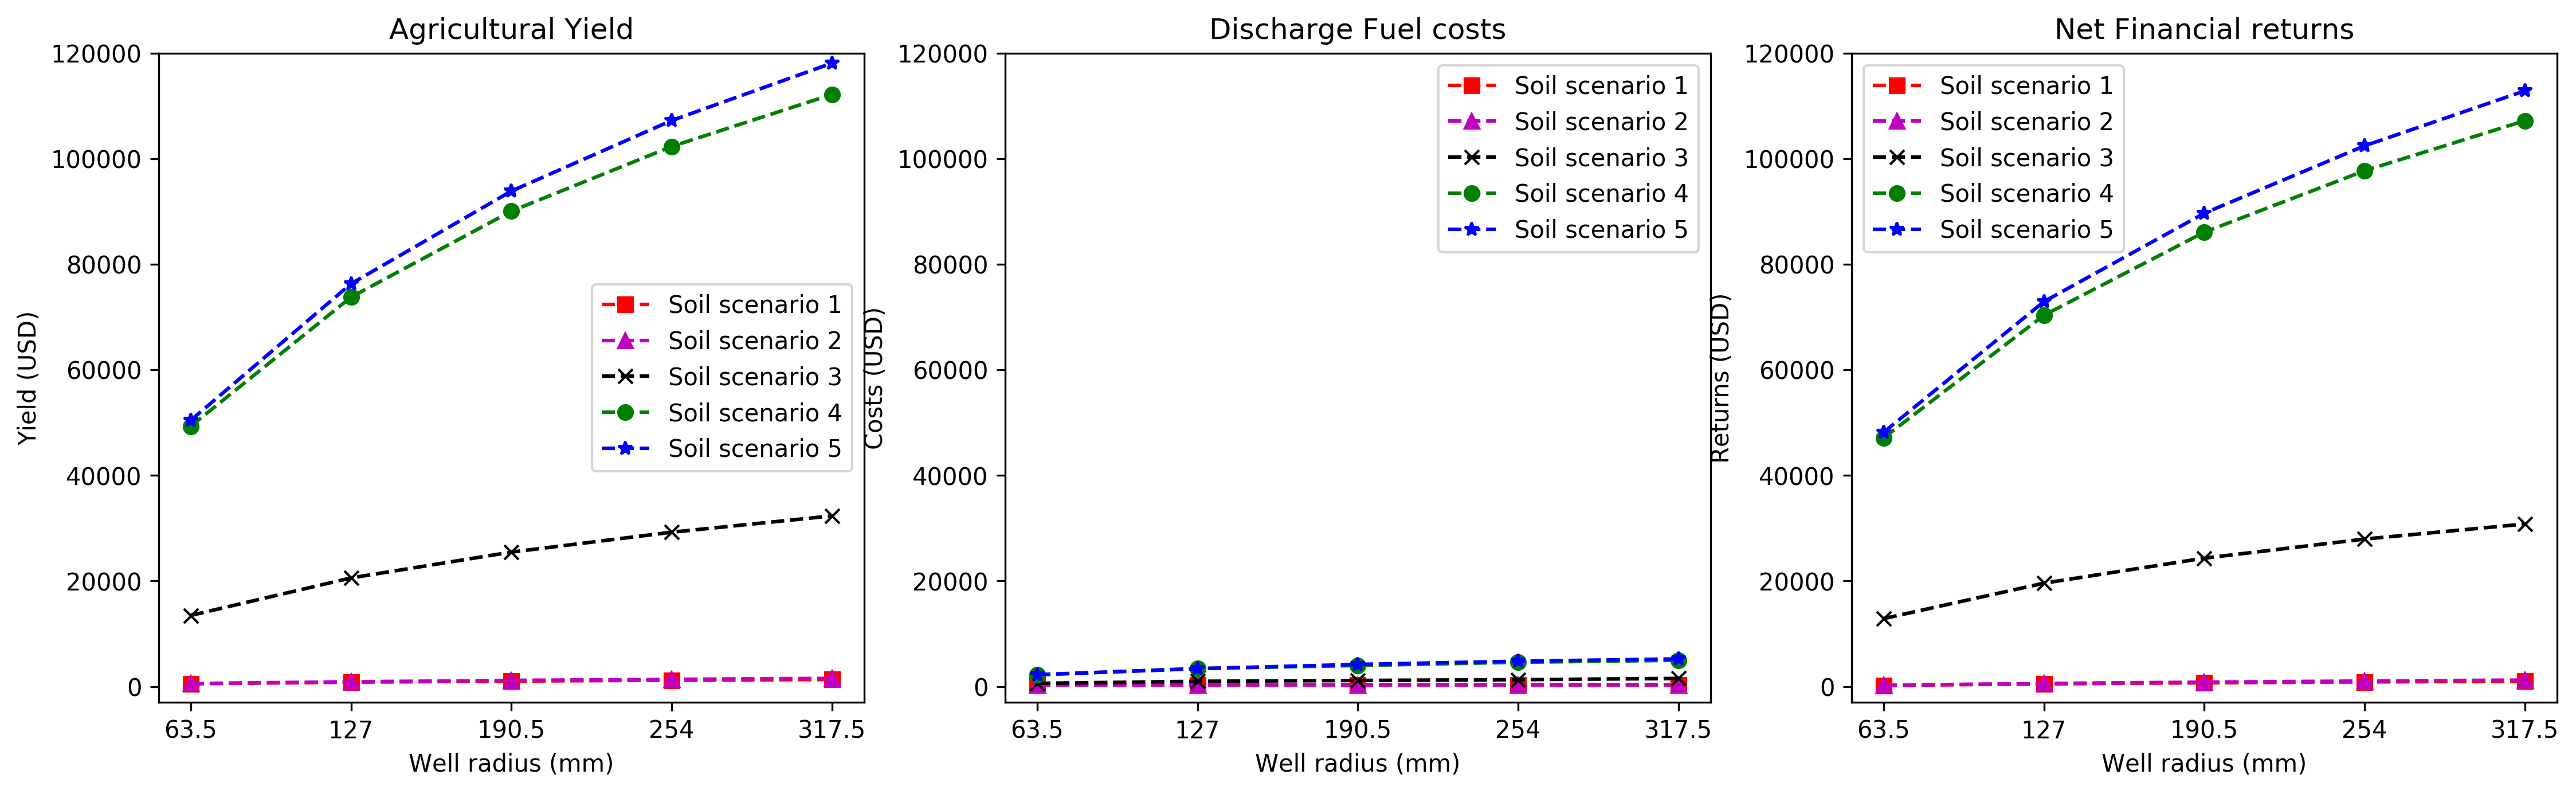
\includegraphics[width=1.0\linewidth]{Results_financial_up_diam}
% \captionsetup{justification=centering} 
% \caption{Well diameter upscaling dependent results on net agricultural yield, costs and net returns}
% \label{fig:Results_financial_up_diam}
%\end{figure}
%
%\begin{figure}[h!]
% \centering
% 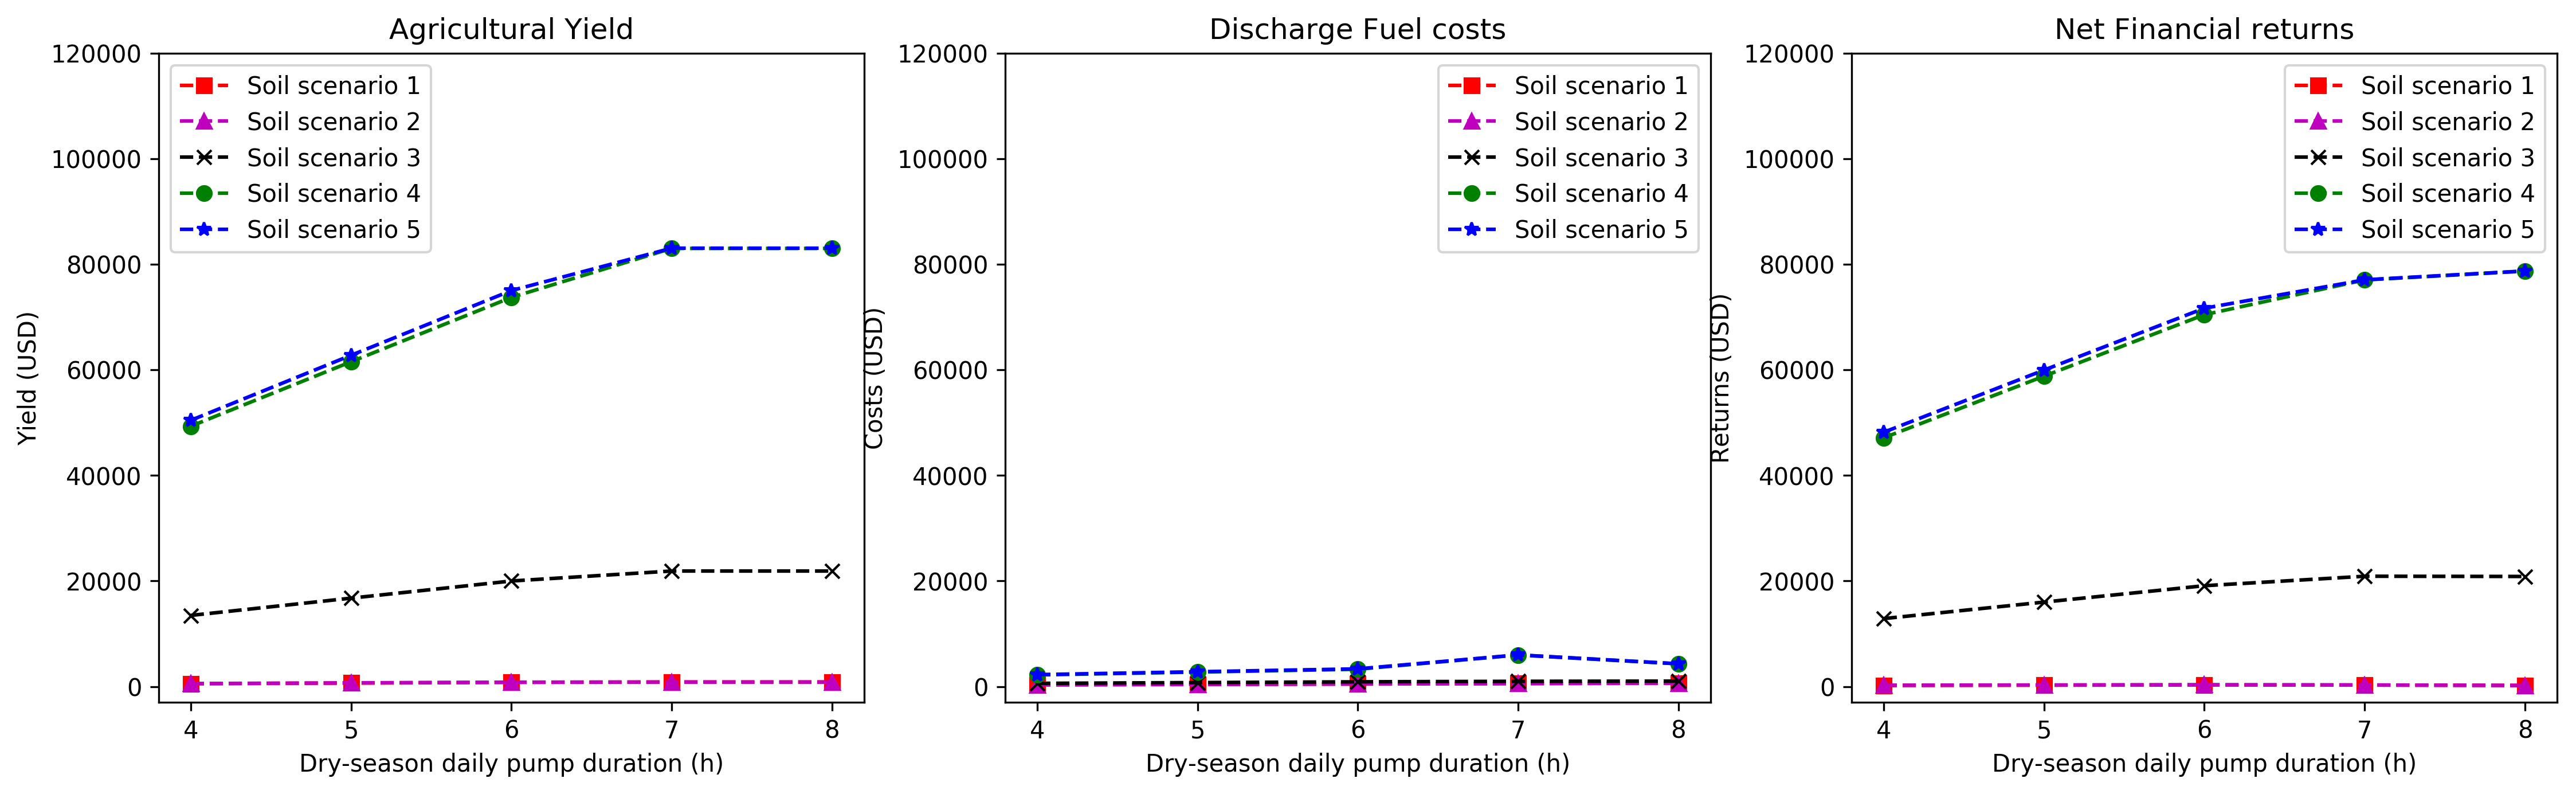
\includegraphics[width=1.0\linewidth]{Results_financial_up_time}
% \captionsetup{justification=centering} 
% \caption{time enlarged results on net agricultural yield, costs and net returns}
% \label{fig:Results_financial_up_time}
%\end{figure}
%
%\begin{figure}[h!]
% \centering
% 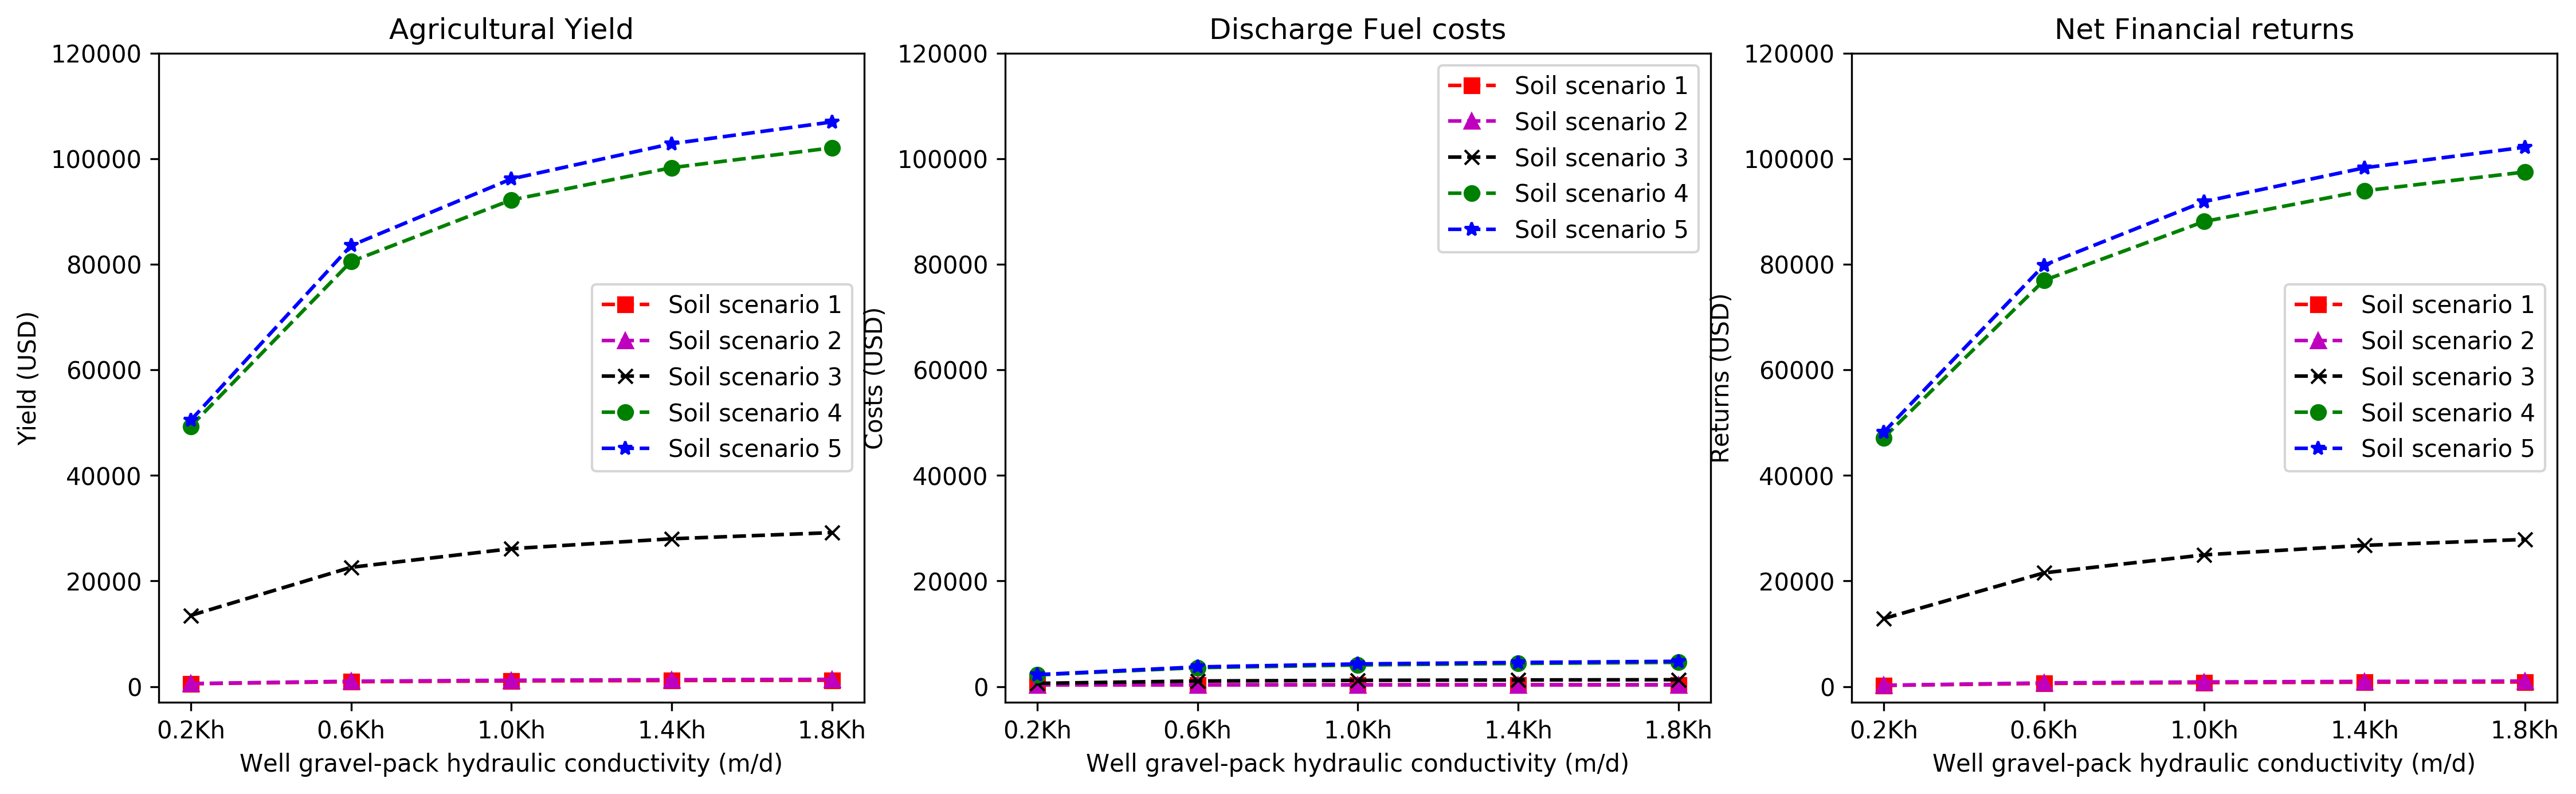
\includegraphics[width=1.0\linewidth]{Results_financial_up_screen}
% \captionsetup{justification=centering} 
% \caption{screen improved results on net agricultural yield, costs and net returns}
% \label{fig:Results_financial_up_screen}
%\end{figure}

\section{Pumping costs}
\label{section:pump_costs}
By the introduction of this section, the acquired ASR system revenues are accompanied by system operational costs. The costs included, are the expenses incurred by the generator diesel fuel consumption (daily pump operation). The remainder of CAPEX (e.g. system installation and pump purchase) and OPEX (e.g. farmer loans and fertilizer costs) is ignored. In northern Ghana practical ASR system implementation it is not unthinkable that elements (e.g. pump and borehole installation) and costs are optimally covered by funds. Nevertheless, the pumping costs are predominantly included to give solely an impression of the (improved) operational feasibility of an ASR system in northern Ghana. \\

The costs for the withdrawal of groundwater (total volumes presented in Section \ref{subsec:improvements}) are for each soil scenario and for each type of ASR system improvement (multiple steps) presented in Figure \ref{fig:tom_gn_yield}. For the simulation of eight months of daily discharge, the operational costs may reach from hundreds upto thousands of dollars (dependent on the volumes and conditions). Herewith, the operational expenses (eight months) are minor relative to the obtained tomato yields, but quantitatively comparable with the revenues of a single groundnut cropping season. 

\begin{figure}[h!]
 \centering
 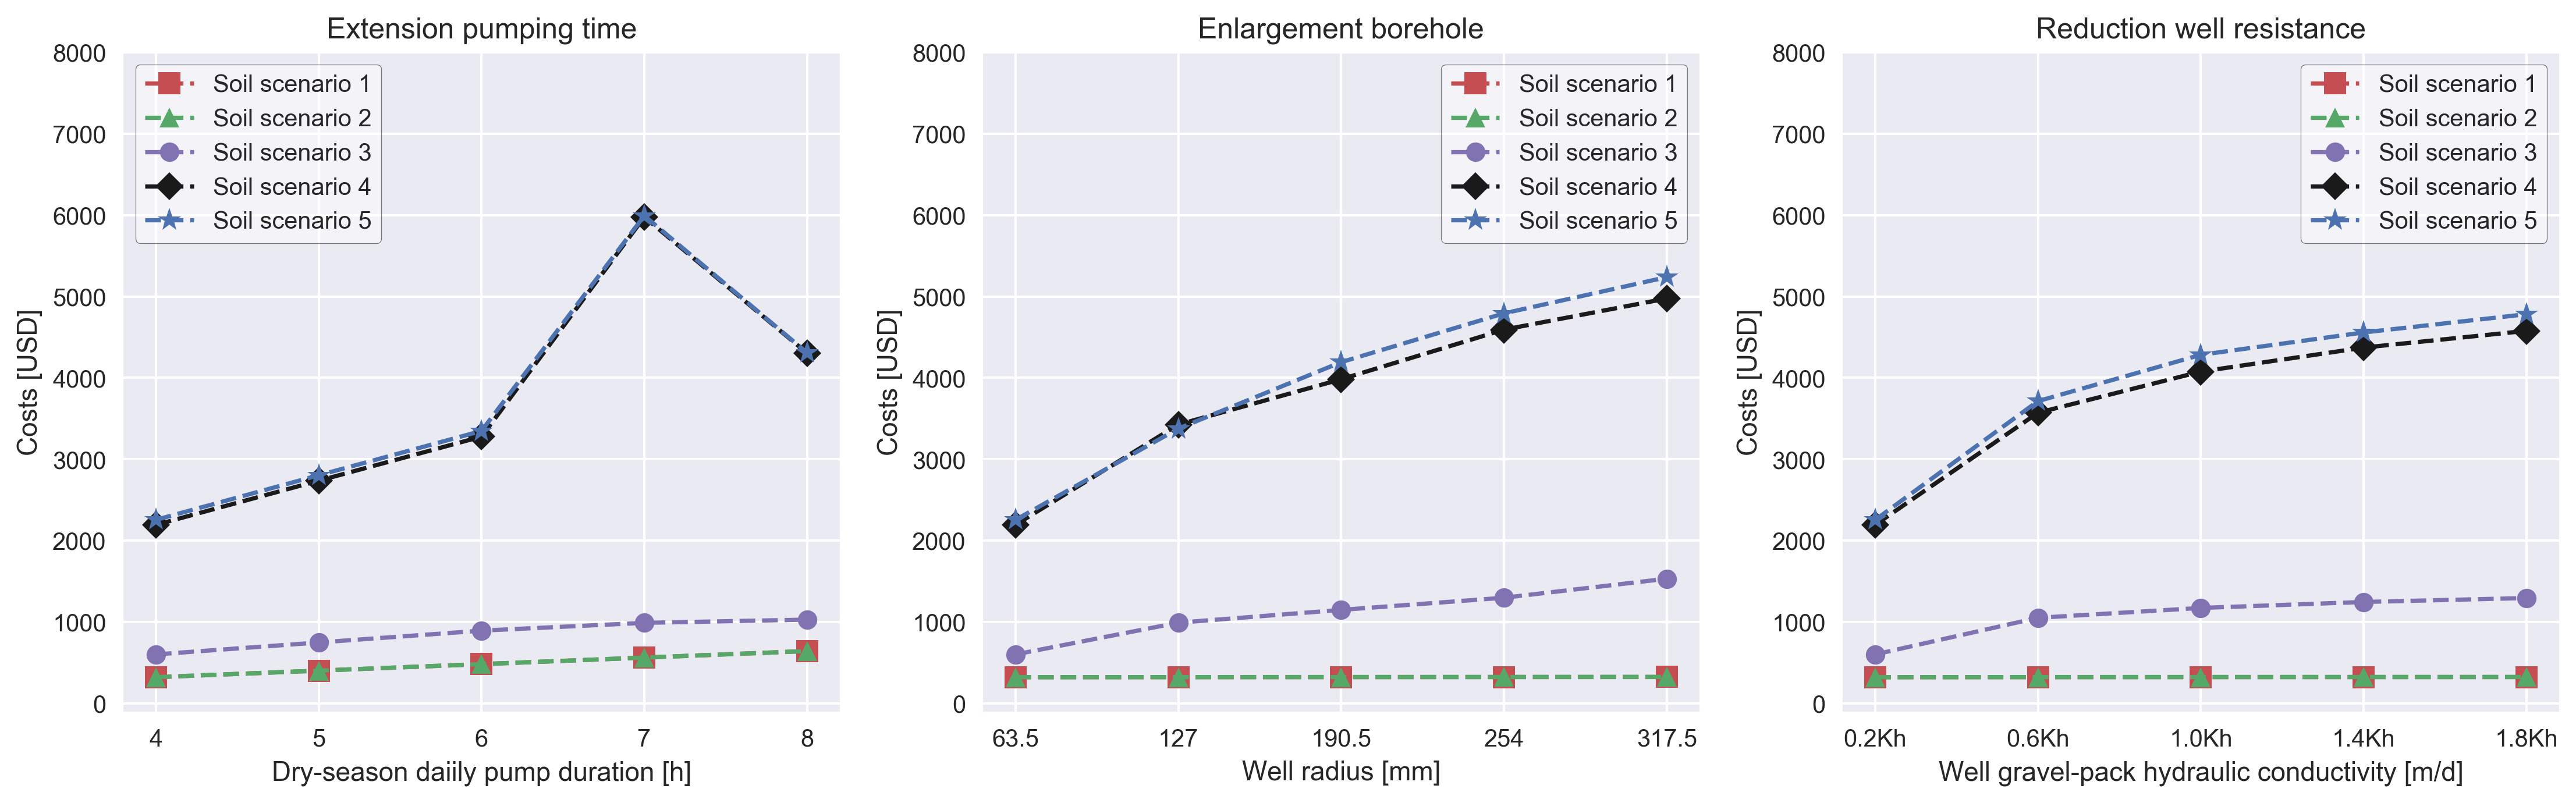
\includegraphics[width=1.0\linewidth]{tom_gn_costs}
 \captionsetup{justification=centering} 
 \caption{Pumping costs - dry season (8 months) - three types of ASR system improvement}
 \label{fig:tom_gn_yield}
\end{figure}

In the comparison of the soil scenario 1 and 2 versus soil scenario 3 substantial deviations are present in the simulated total volumes discharged (Section \ref{subsec:improvements}). As visible in Figure \ref{fig:tom_gn_yield}, these deviations are less dominantly present in the pumping costs. This is most clearly visible for the base model simulations (absolute left-side of Figures) and the simulations with an ('improved') extension of the daily pumping time. The reduced deviation in costs can be attributed to the applied pump efficiencies. The pumping curve of the Pedrollo 4" submersible pump is defined as normative (Appendix \ref{chapter:Pedrollo_product_specs}). The discharge rates obtained in the simulations of soil scenarios 1 and 2 do not ideally match the specification of this pump. As a result, low(er) pumping efficiencies are implemented and high(er) discharge costs are sorted. \\

%The obtained (model) discharges for the soil scenarios 1 and 2 are extremely low. As a consequence, pumping efficiencies (Pedrollo 4" submergence pumping curve) are stated to be almost zero. A situation highly unlikely. In practise, a specific pump type will be applied that suits the circumstances. As a consequence, unrealistic judgements and comparisons are applied.

Besides, the Pedrollo 4" submersible pump has, like every pump, its own specific discharge limits. The obtained discharge rates for the soil scenario 4 and 5 simulations (base model and improved system) are out of pumping range. An inconvenience, worked around by the (simulated) installation of one or more additional pumps. By this approach the specified discharge rates are (theoretically) met. As an adverse affect, moderate pumping efficiencies can occur when the number of pumps is stepped up. Herewith, the outliers (peak) in operational cost for the soil scenario 4 and 5 ('improved') seven hour daily pumping operation (Figure \ref{fig:tom_gn_yield}) can be justified. \\  

%Note, the outlier in the soil scenarios 4 and 5 for the situation of 7 hours pumping operation can be justified by the application of an unfortunate number of pumps. Efficiencies are in this particular case relatively low (as low as 35\%). \\

The installation of a too powerful pump and the use of abundant number of pumps (in parallel) are both situations that are practically unlikely and undesired (low efficiencies and high purchase costs). Figure \ref{fig:tom_gn_yield_maxeff} presents the ASR system operational costs for each soil scenario and for each type of improvement (multiple steps), when maximum pumping efficiencies are taken into account. Based on the specifications of the Pedrollo 4" submersible pump a maximum pumping efficiency of 58\% is implemented (Appendix \ref{chapter:Pedrollo_product_specs}). A comparison of the Figures \ref{fig:tom_gn_yield} and \ref{fig:tom_gn_yield_maxeff} learns, optimal pumping efficiencies can (sometimes) significantly lower the systems operational costs. For a high efficient use of the ASR system, one should tune the applied pump (pumping curve) to the local circumstances. 

%Substantial deviations in the total groundwater withdrawn volumes (Section \ref{subsec:improvements}) are (amongst others) present between the soil scenario 1, 2 and soil scenario 3.

%Two developments present in the results of Figure \ref{fig:tom_gn_yield} require a specification. Despite the substantial deviation in total volumes withdrawn (Section \ref{subsec:improvements}), the base model operational costs (absolute left-side in Figures) for the soil scenarios 1 and 2 do not deviate much from the costs to obtain the water volumes in soil scenario 3.

%However, the increase in pump numbers is not reflected in this research costs. As a consequence, unrealistic judgements and comparisons are applied. \\

%can be attributed to an inconvenient change in the number of pumps required to deliver the specified discharge rates. 

\begin{figure}[h!]
 \centering
 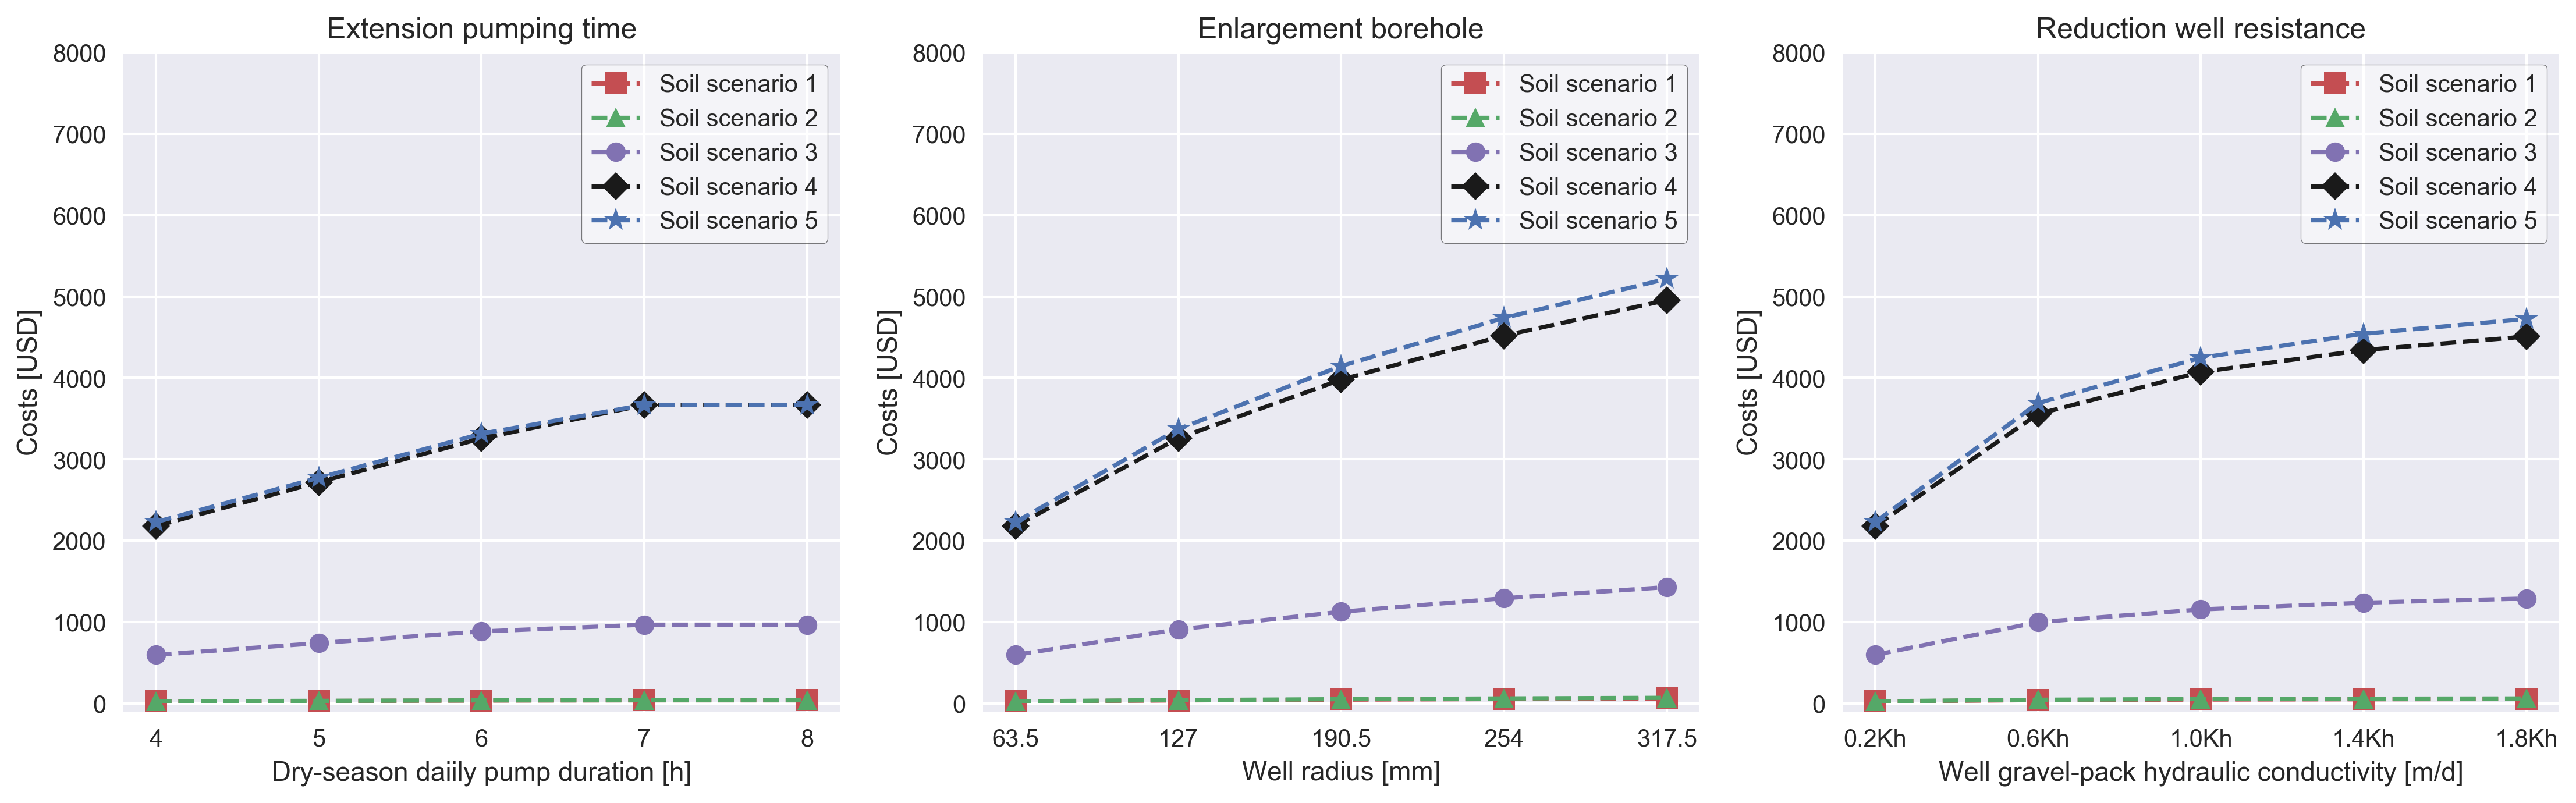
\includegraphics[width=1.0\linewidth]{tom_gn_costs_maxeff}
 \captionsetup{justification=centering} 
 \caption{Pumping costs - maximum pumping efficiency - dry season (8 months) - three types of ASR system improvement}
 \label{fig:tom_gn_yield_maxeff}
\end{figure}

An overview of the business case financial returns is presented in Appendix \ref{section:bus_case}. The ASR system financial returns for both, the 'actual' and the optimal pumping efficiency costs are included. \\ 

%
%note, the remainder of OPEX and CAPEX is undetermined. deze kosten kunnen echter deels opgevangen worden door europese fondsen (niet ondenkbaar). Daardoor wordt de  costs are undetermined. 
%
% Therefore, the business case is not quite representative for the actual het zegt alleen solely mogelijk iets over het (beter kunnen) gebruik van het ASR system in northern Ghana. 
% 
%door de afwezigheid van dan en dat niet bepaald een business case. maar tegelijkertijd toch ook weer wel. sommige items kunnen mogelijk vergoeding krijgen vanuit (europese) fondsen. Waardoor de financial balance al weer iets representatiever geinterpreteerd kan worden. 
%
% due solely the withdrawal of water,
% gekozen voor een zeer onrealistische financiele situatie, omdat informatie gewoon afwezig is. capex (denk aan pomp costen zelf. plaatsing van de well, land, irigatie systeem, polytanks) opex (denk aan famers loans, fertilizers) Bovendien kunnen onderdelen vanuit (europese) fondsen in aanmerking komen voor een fianciele compensatie. waardoor het financiele kostenplaatje al weer iets minder onrealistisch is. nonetheless, business case blijft hoogst onzeker. verder onderzoek dan ook zeker wenselijk. 

\section{Results \& conclusions}
\label{section:Yields_conclusions}
This section contains the conclusions that can be drawn from the ASR system business case. Key options concerning the agricultural yield and pumping costs are stated, to guarantee efficient (financial) system handling. \\

%and potentially improve the system's financial feasibility. \\

\begin{itemize}
\item{Yield increase} \\
By the implementation of the explored ASR system improvements, increased discharge volumes are acquired and higher financial (and agricultural) yield can be expected. A crop-specific yield comparison (Tomato versus Groundnut) reveals, the financial yield is potentially more dominantly affected by crop cultivation choice rather than the implementation of one of the investigated system improvements. Nonetheless, the crop-specific market price remains decisive in the ASR system financial feasibility.  

%met de juiste keuze in crop type kunnen de operational costs worden omgezet in profits. de system improvement kan hier een moderate role bij spelen, maar die invloed kan mogelijk wel net het verschil maken. (dit misschien in de discussie. hou het hier clinisch met kosten en opbrengsten). 

%Under the defined research conditions, it definitely pays-off to pick the ‘right’ crop. In terms of financial profit, the magnitude is more dominantly affected by crop choice, rather than ASR system improvements.

\item{Operational cost reduction} \\
The ASR system operational costs are influenced by the withdrawal efficiencies. For an efficient use of the ASR system, the applied pump (pumping curve) should be specifically tuned to the local possibilities in groundwater discharge rates. The natural geohydrological conditions and the system composition play a role in this process. The selection of the 'right' pump can make the difference in the financial feasibility of an ASR system. 

%Efficiencies are influenced by the achievable discharge rates (based on ASR system and soil conditions). Potential ASR system modifications and natural conditions play a role in this process. \\

\item{Additional research} \\
The business case contains strong simplifications, uncertainties and is far from complete. Multiple additional components in CAPEX and OPEX can be added. It is unknown to what extent ASR system components are eligible for funds. For a more detailed financial feasibility of an ASR system implemented in northern Ghana, future financial research is advisable. \\ 
\end{itemize}

%gekozen voor een zeer onrealistische financiele situatie, omdat informatie gewoon afwezig is. capex (denk aan pomp costen zelf. plaatsing van de well, land, irigatie systeem, polytanks) opex (denk aan famers loans, fertilizers) Bovendien kunnen onderdelen vanuit (europese) fondsen in aanmerking komen voor een fianciele compensatie. waardoor het financiele kostenplaatje al weer iets minder onrealistisch is. nonetheless, business case blijft hoogst onzeker. verder onderzoek dan ook zeker wenselijk. 


\chapter{Conclusions}

Final conclusion will follow soon \\

Final conclusions can only be made if the thesis core in terms of content is fixed. \\
Chapters do contain sub-conclusions / summaries \\



 

\textbf{Research question}\\

How can scaled-up Aquifer Storage and Recovery (ASR) systems be beneficial for the availability and sustainable use of groundwater in northern Ghana small-scale agriculture? \\

\chapter{Discussion \& Recommendations}

good, bad, advice further research


%\bibliographystyle{apa}
\bibliographystyle{apalike}
%\def\biblio{\bibliographystyle{apalike}\bibliography{Mendeley_v1}}
\bibliography{Mendeley_v1}

%% Use letters for the chapter numbers of the appendices.


\appendix
%\input{appendix-a}
\chapter*{Appendices}
\addcontentsline{toc}{chapter}{Appendices}
% geforceerd toevoegen aan contents lijst
\chapter{Original borehole log sheets}
\label{chapter:Borehole_logsheets}

In the first half of the year 2016 Conservation Alliance (CA) commissioned the construction of multiple boreholes in northern Ghana. The boreholes subjected in this research (five locations, visualized in \ref{fig:Overviewlocations})are all part of this operation. Valuable information is gained with respect to local soil stratification, during borehole construction. Information is preserved in the original borehole log-sheets, which can be found in this appendix. Besides the local soil stratification, these log-sheets contain information on individual applied well structures. A depth dependent distinction is made in plain versus screened well skin. In terms of content these borehole log-sheets are used as a starting point in the theoretical model determination (section \ref{section:derivation_methods}). 

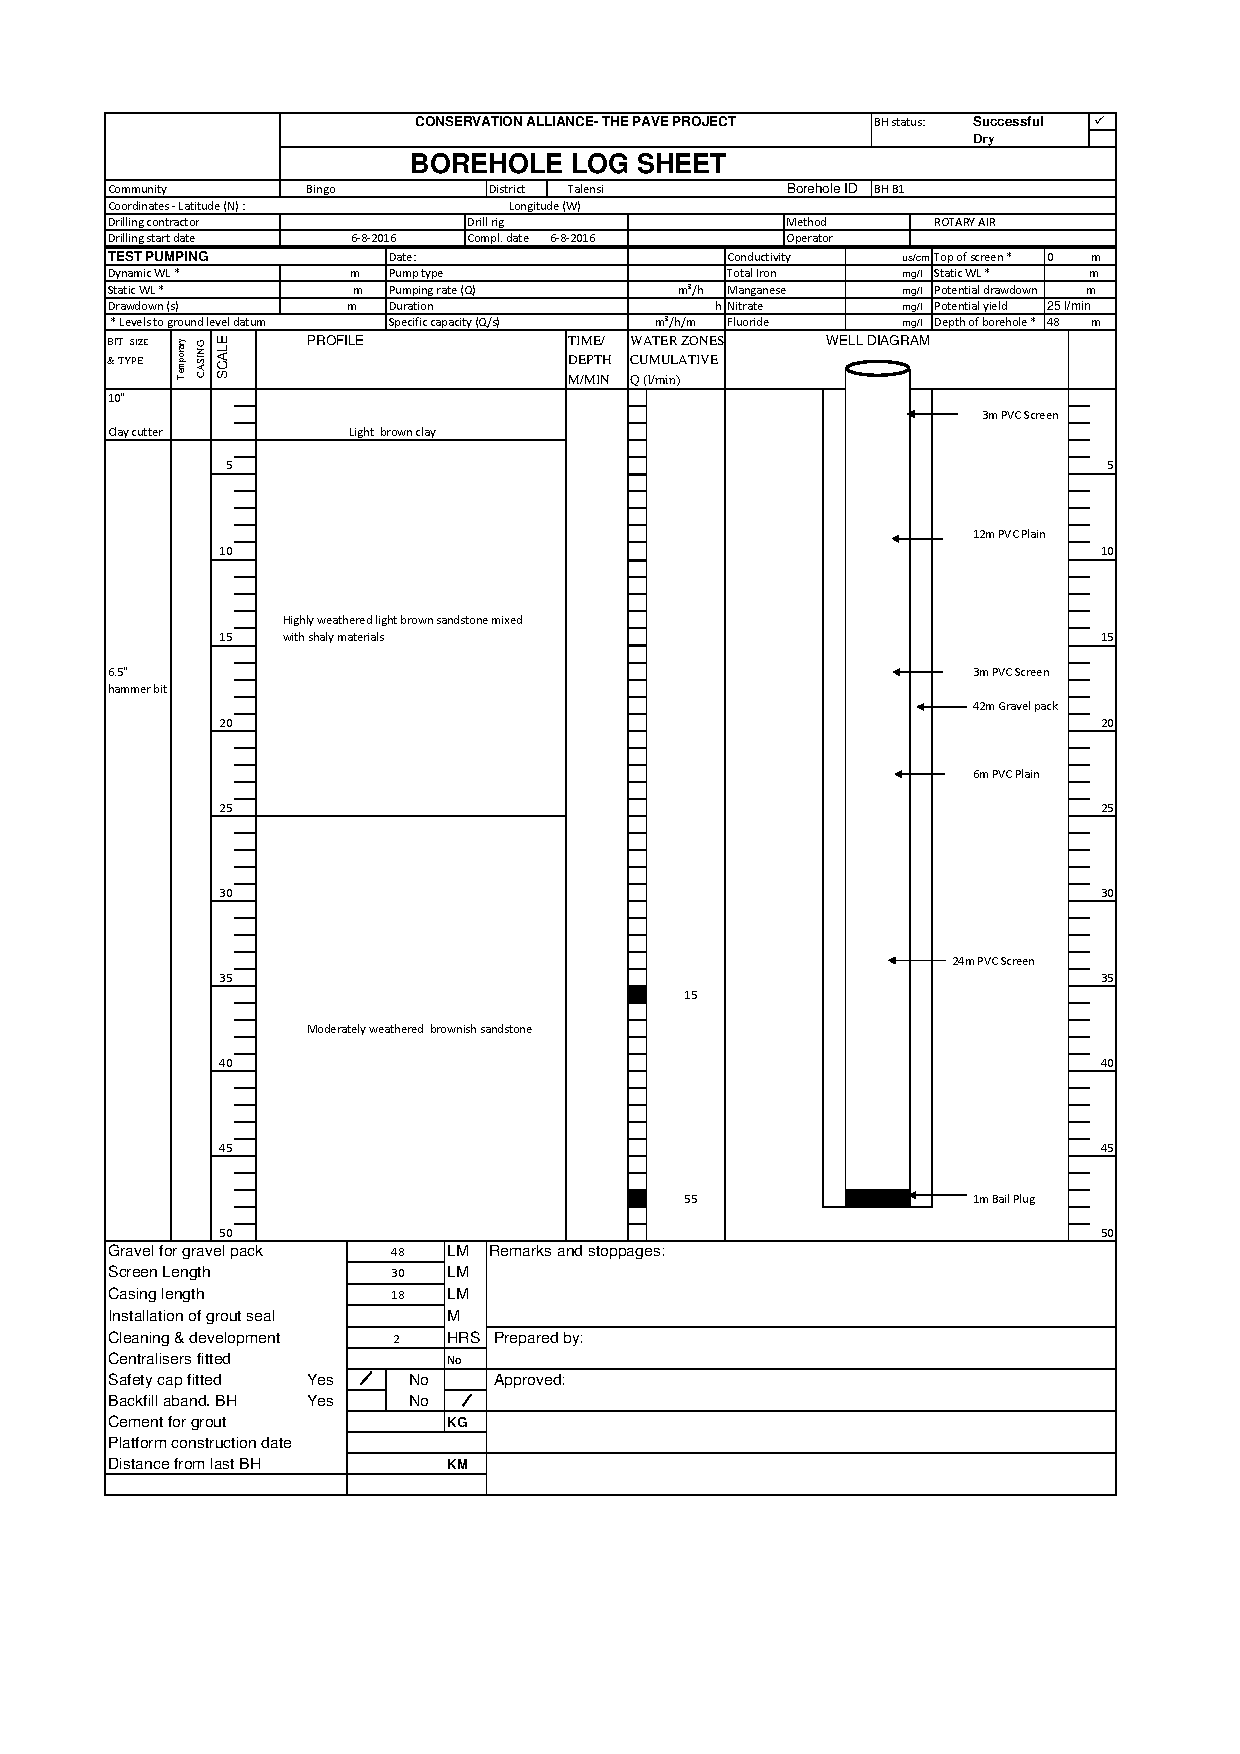
\includepdf[pages={1}]{BH_Bingo.pdf}
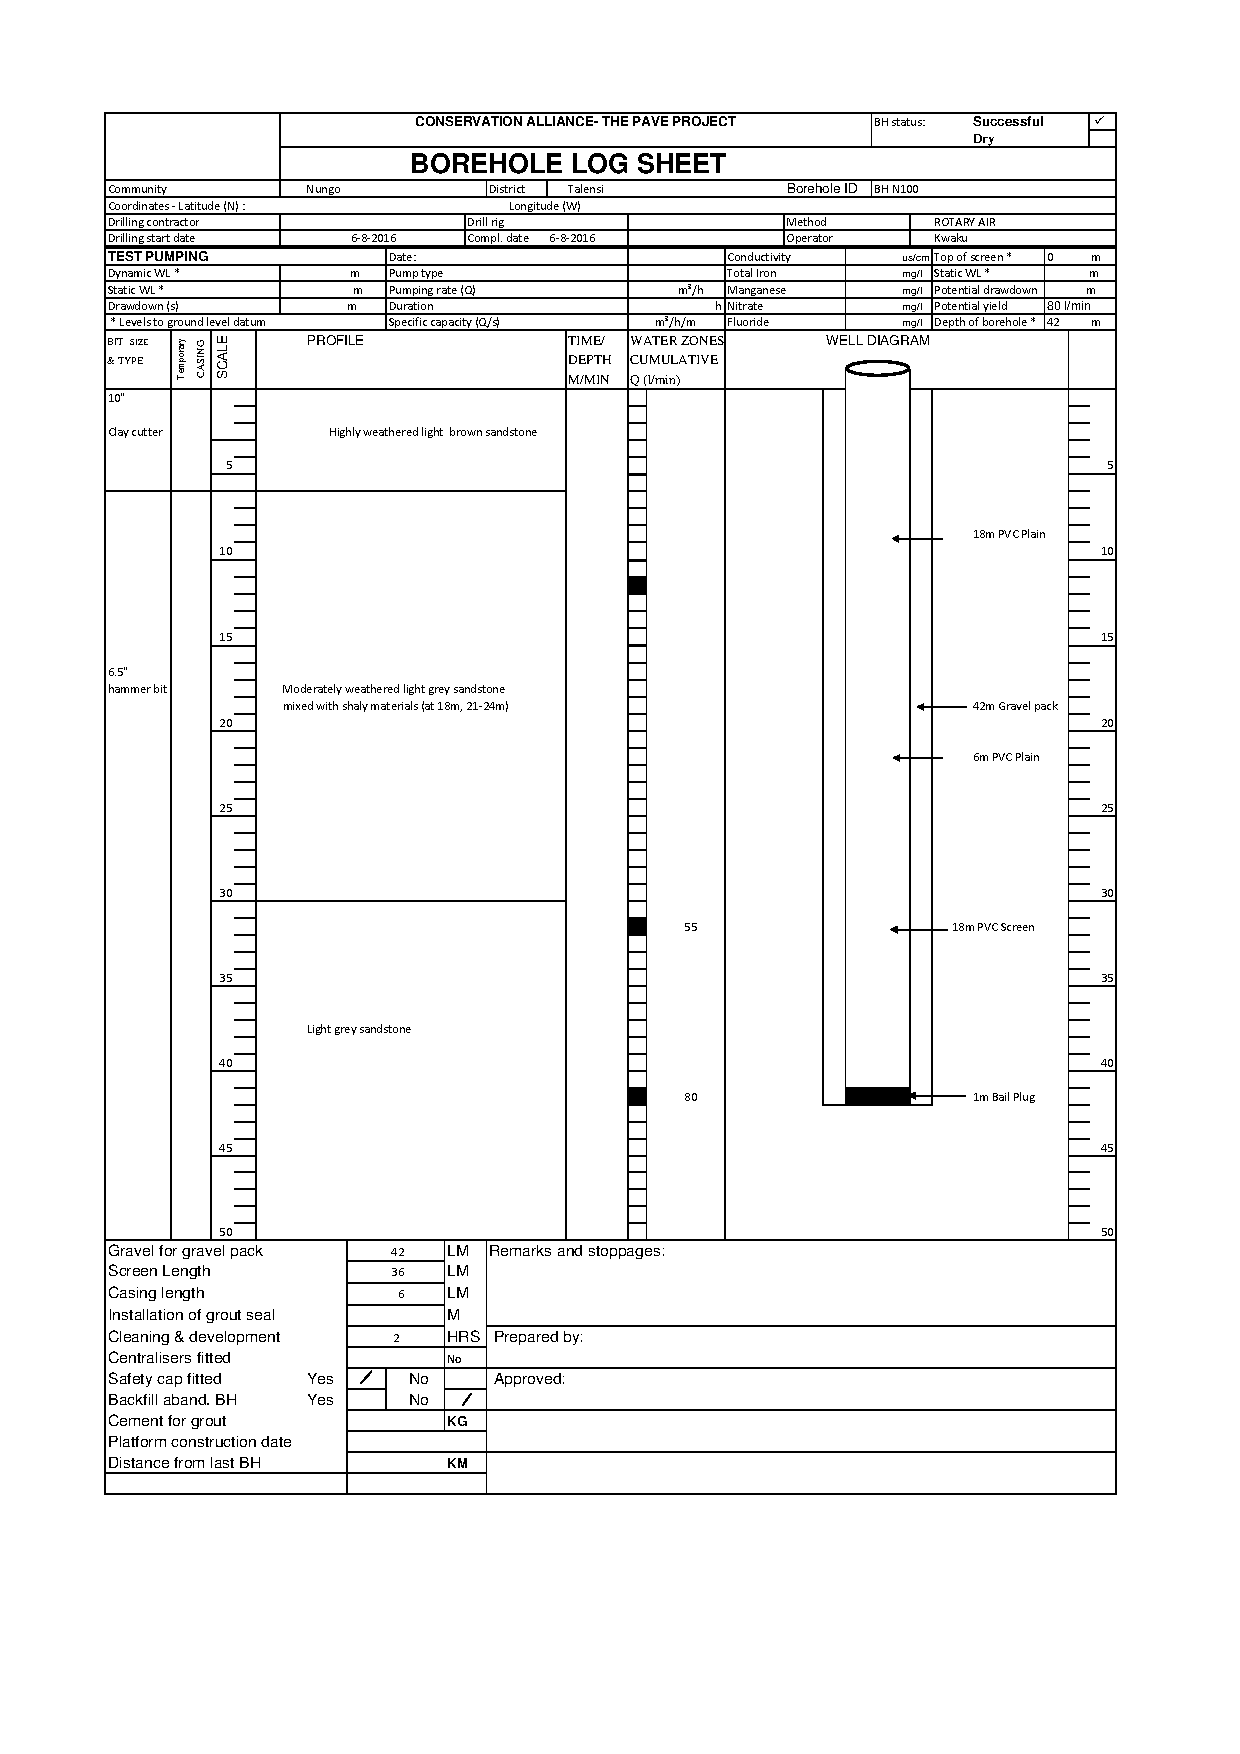
\includepdf[pages={1}]{BH_Nungo.pdf}
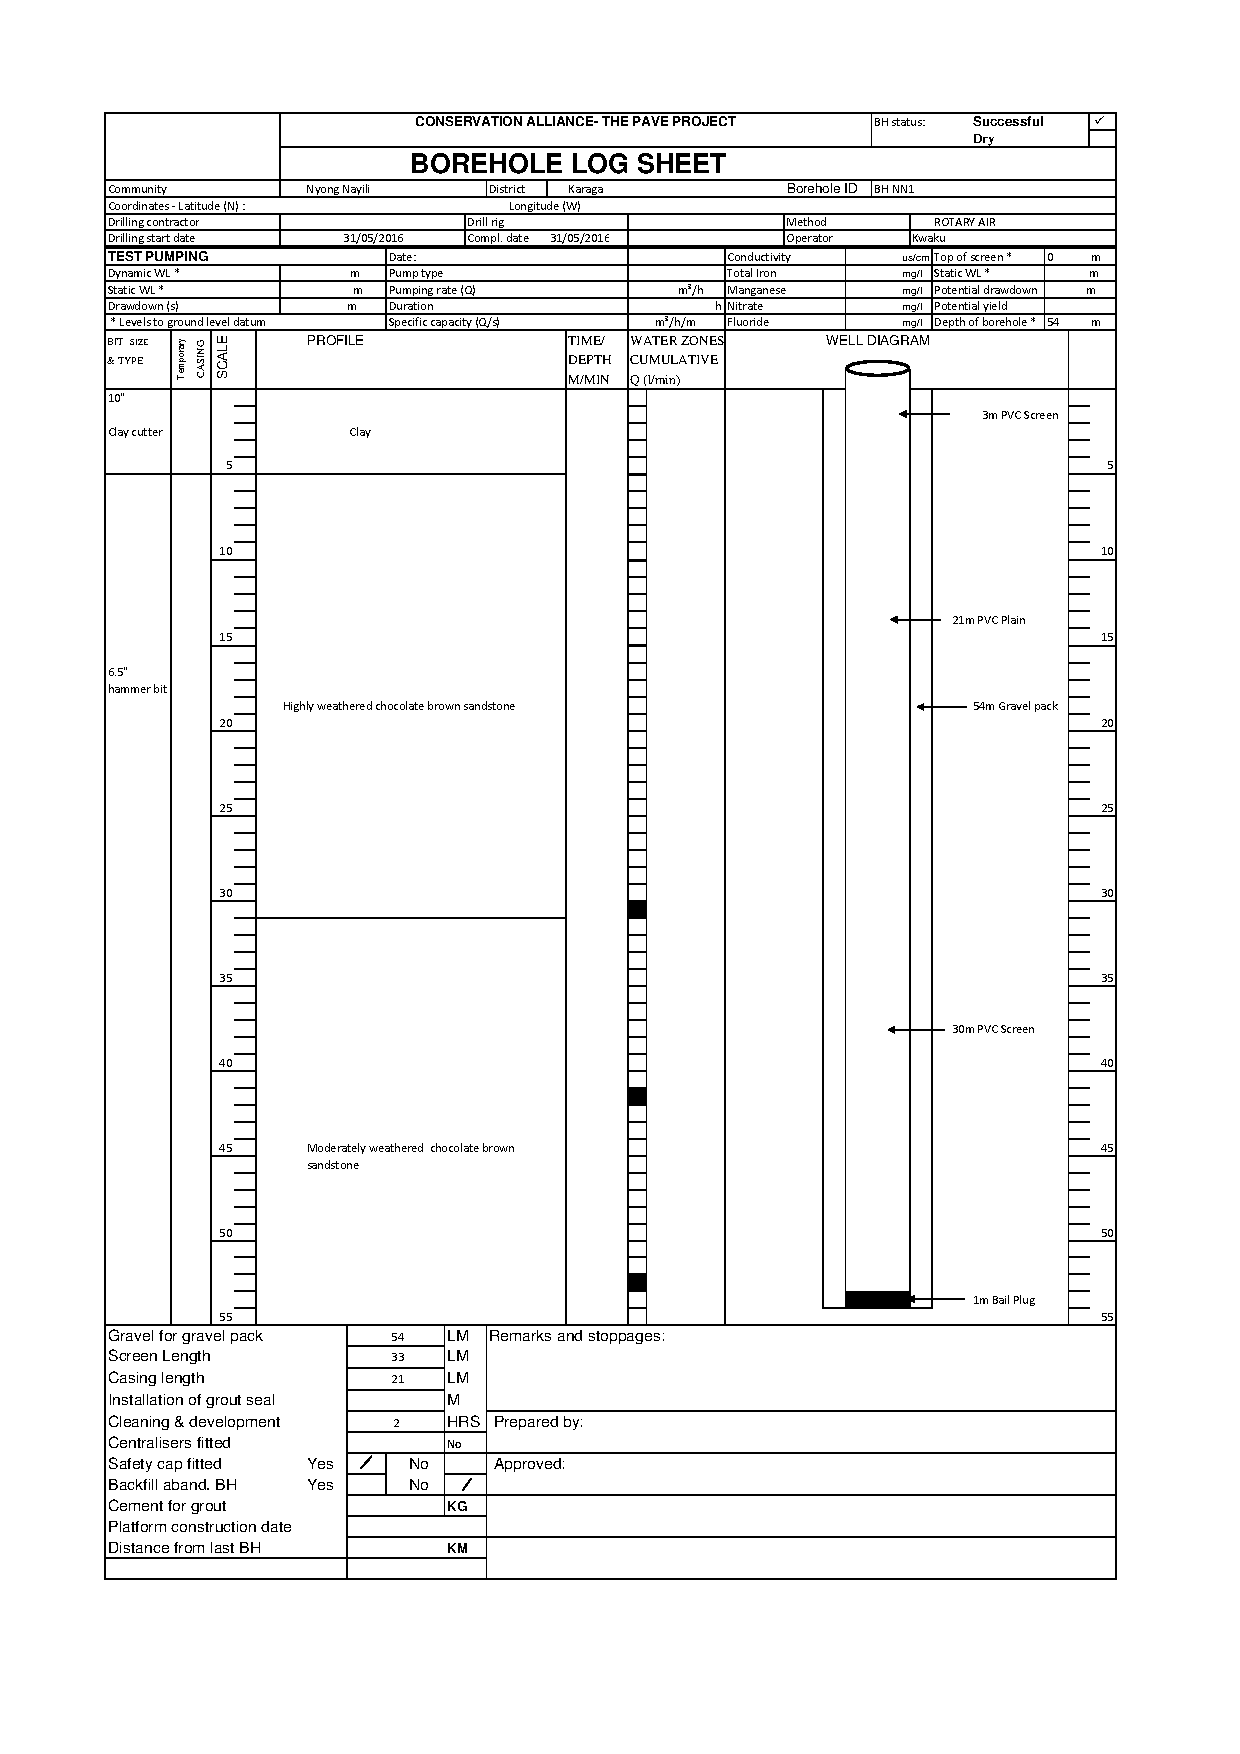
\includepdf[pages={1}]{BH_Nyong_Nayili.pdf}
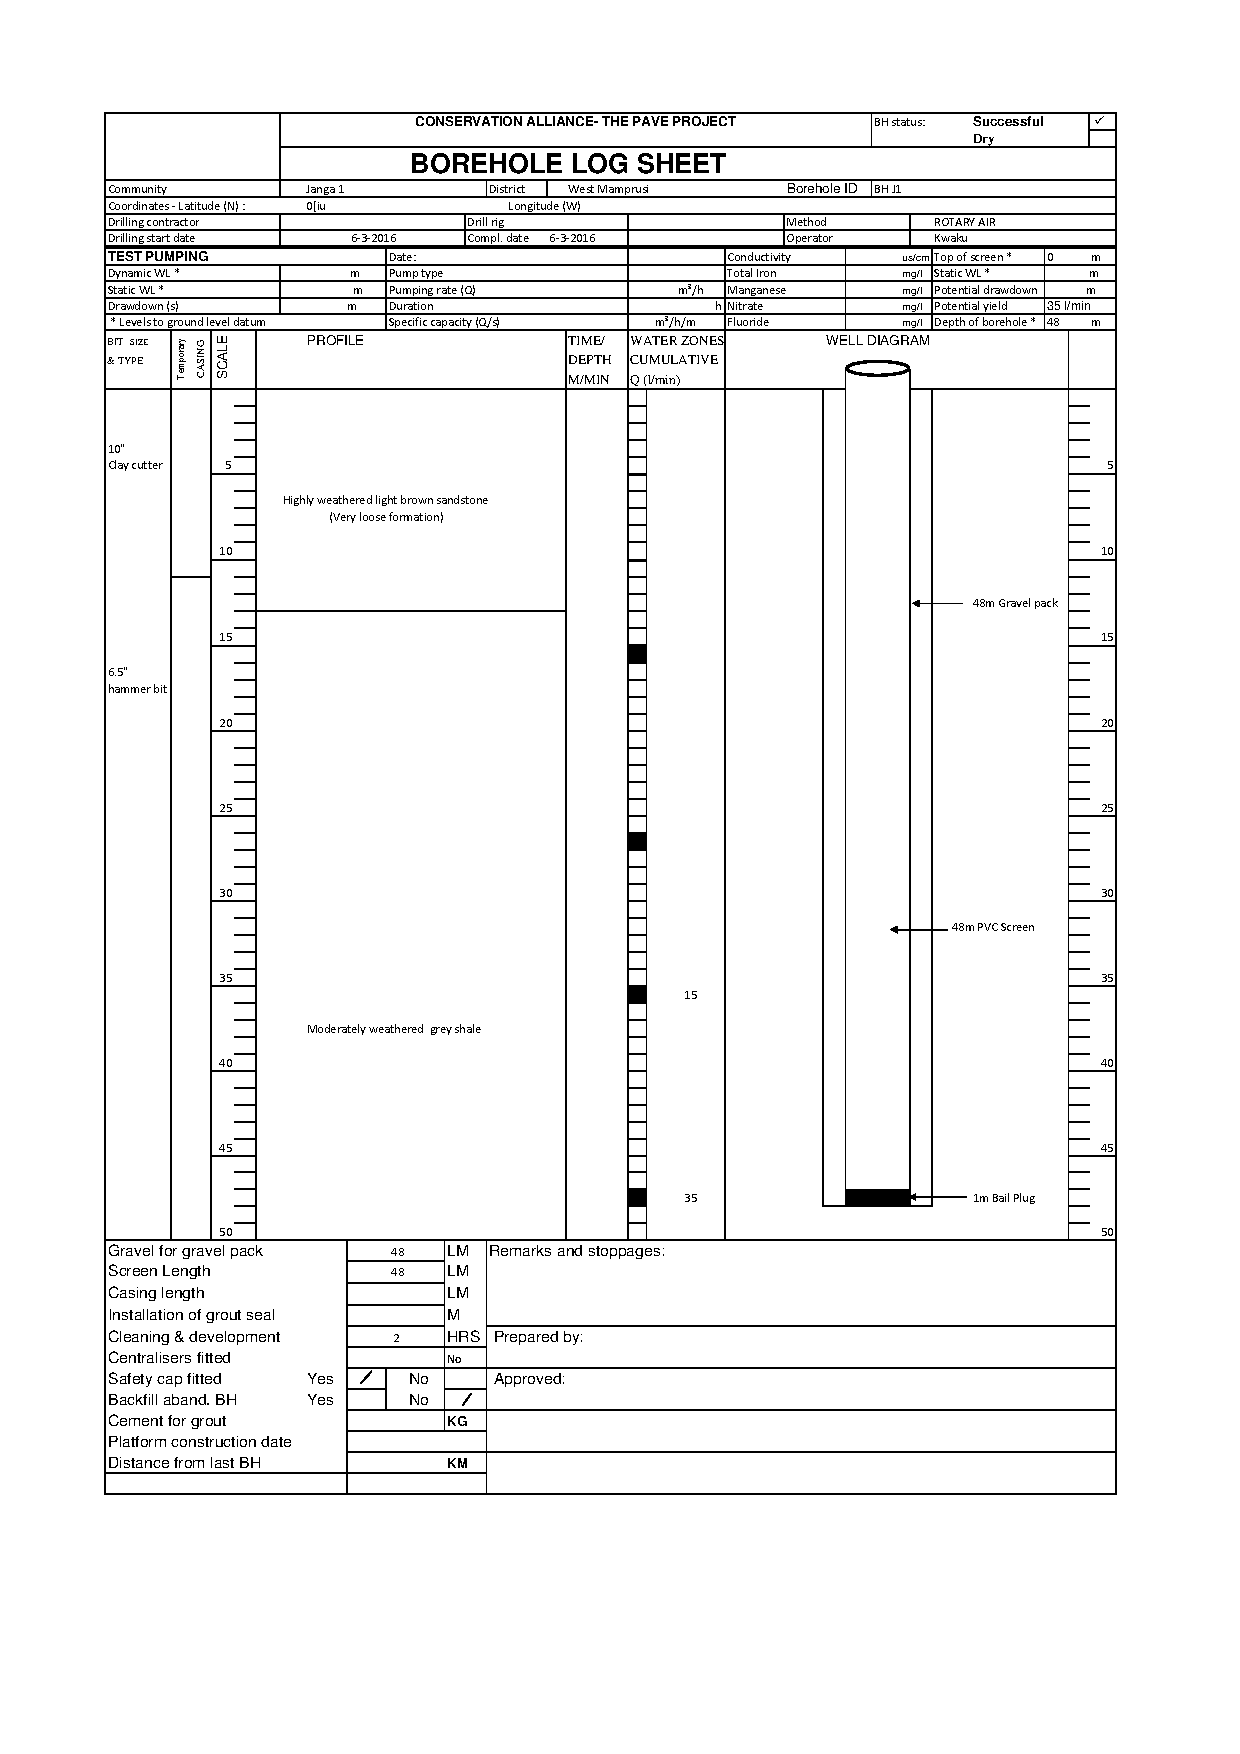
\includepdf[pages={1}]{BH_Janga.pdf}
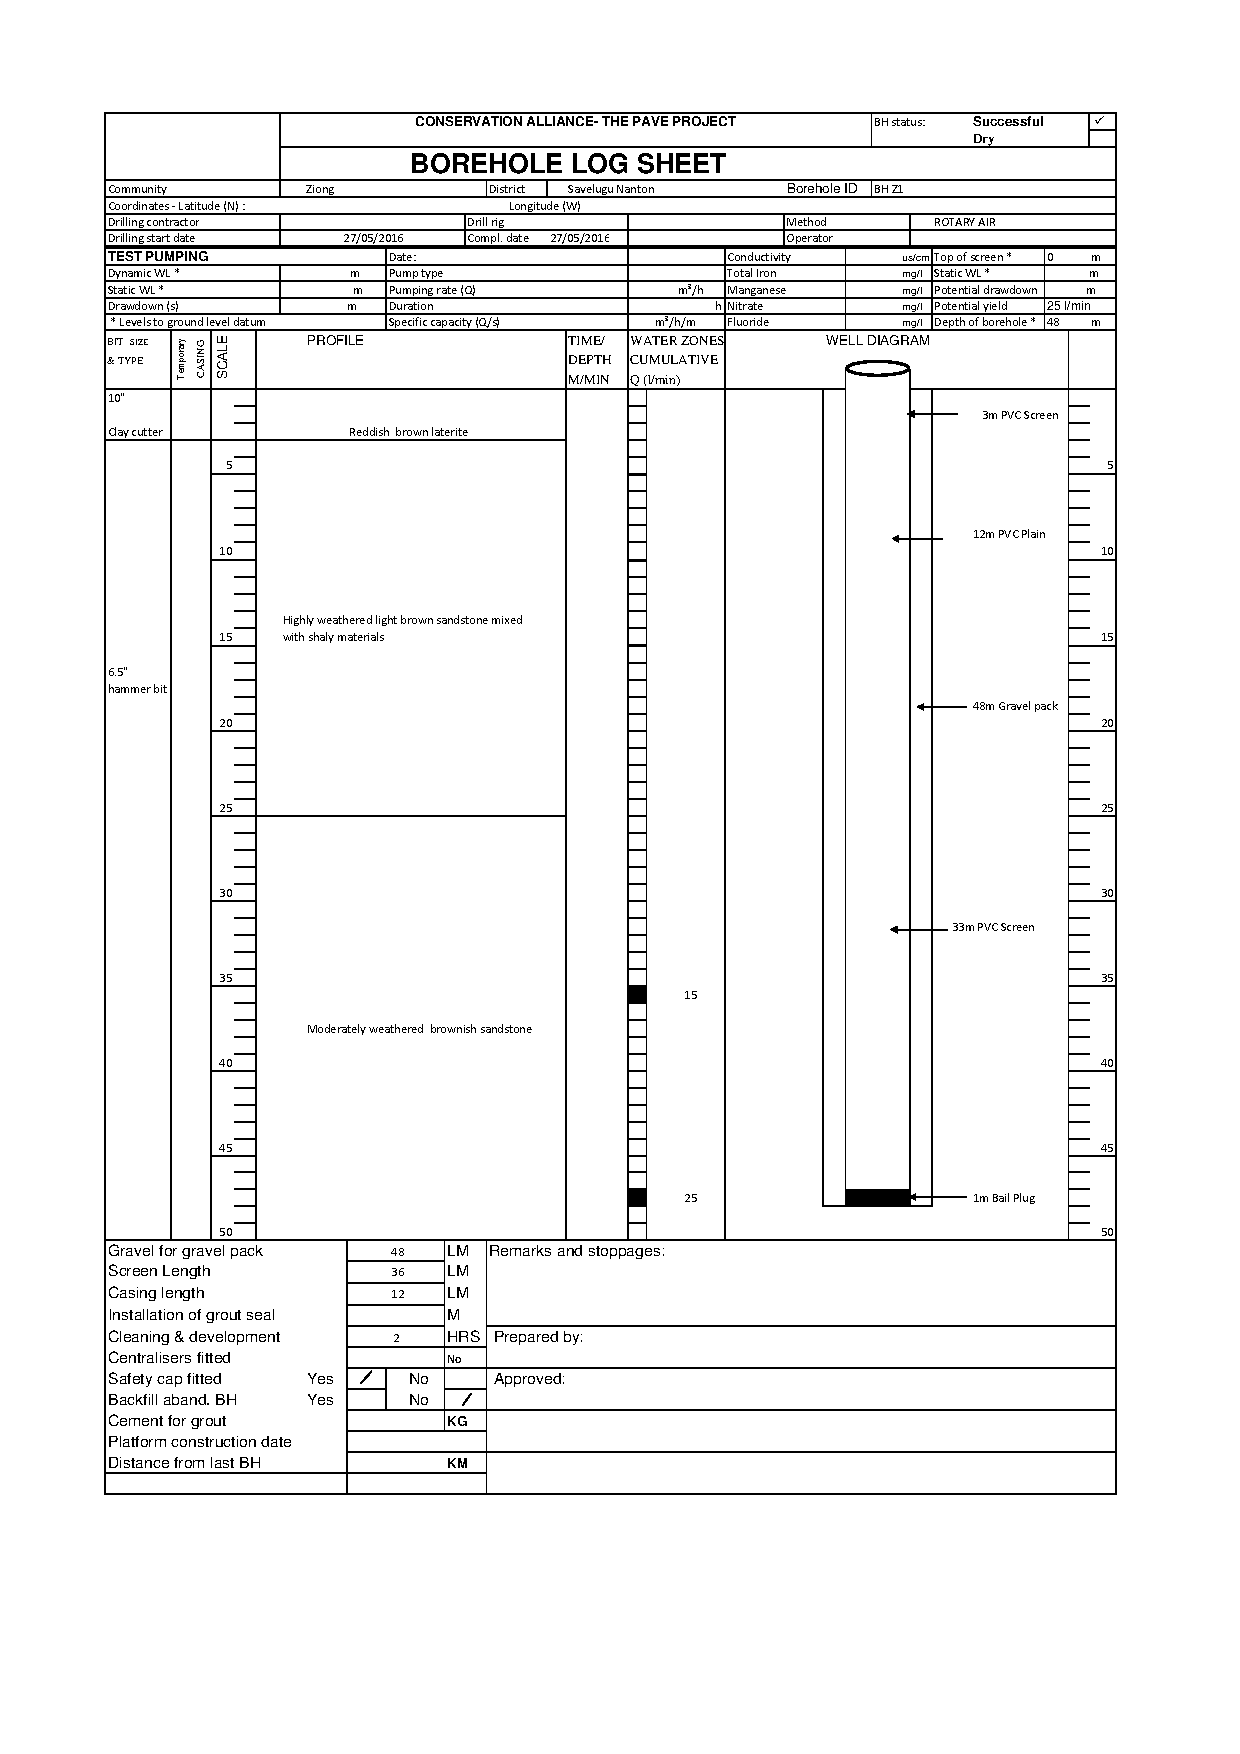
\includepdf[pages={1}]{BH_Ziong.pdf}
\chapter{Aquifer test - Equipment}
\label{chapter:fieldwork_set-up}

The northern Ghana in-field geohydrological data collection would not have been possible without the interference of Conservation Alliance (CA). Spread over the Upper East and Northern Region the NGO holds multiple PIT locations. Five locations, visible in figure \ref{fig:Overviewlocations}, are appointed as measurement locations for the purposes of this research.
Besides the research locations, CA provided transport, an interpreter and pumping test equipment. The section below contains detailed information on the equipment applied. A distinction has been made between the equipment for the pumping tests and the actual groundwater measurements. Moreover small equipment as pliers, screwdrivers, gloves and robes are ignored. Purposes and use of these tools are taken for granted.\\
% Moreover, it describes the general fieldwork pumping test / monitoring set-up. The section concludes with fieldwork fact-sheets, containing the collected data for each individual location. 
%The applied in-field pumping tests are executed with a same set of equipment. The paragraph below contains a detailed description of the most important tools. In this case a distinction has been made between the equipment for the pumping tests and the actual groundwater measurements. Moreover small equipment as pliers, screwdrivers, gloves and robes are ignored. Purposes and use of these tools are taken for granted. \\

\section{Pumping test} 

\begin{itemize}
\item Pump: Pedrollo 4” submersible pump; Type 4SR4/18 \\
A 2 HP pump, for example usable for the supply of water to irrigation fields. While pumping the water should preferably not exceed 35 $^{\circ}$C and should not contain too many particles; no more than 150 g/m$^{3}$. The pump can be submerged in water up to 100 meters. Installed in the right way, the pump can deliver 20-100 l/min with an head difference of 112-45 m. More specific information regarding the pump can be found on the Pedrollo webpage.

\begin{figure}[h!]
 \centering\includegraphics[width=0.35\linewidth]{Pedrollo}
 \captionsetup{justification=centering}
 \caption[Comparable example of the fieldwork submersible pump]{Comparable example of the fieldwork submersible pump \\ (source: \url{https://www.pedrollo.com/en/4sr-4-submersible-pumps/150})} 
 \label{fig:Pedrollo}
\end{figure}

\item Generator \& power converter: Kipor diesel generator - 5 kVA \\
A mobile generator has been used as a pump power source. The Kipor generator is a relatively small model, easy to handle and meets the pump requirements by the use of the 230 V connection. A power converter is placed between generator and pump to manually switch on and off the pump. To facilitate a flawless transfer between generator and pump one should be aware the cables and connections towards the pump should be waterproof. Moreover these power cables should be of a decent length to allow the pump to submerge. 

\begin{figure}[h!]
 \centering\includegraphics[width=0.40\linewidth]{Kipor}
 \captionsetup{justification=centering}
 \caption[Comparable example of the fieldwork generator]{Comparable example of the fieldwork generator \\ (source: \url{https://www.kipor-power.eu/winkel/kipor-kde6700t-diesel-generator-5-kva/})}
 \label{fig:Kipor}
\end{figure}

\item Hose: \\
As a transport line towards the location of discharge a flexible water hose has been attached to the pump. The hose has been manufactured in Polyethylene, has an external diameter of 1$^{1⁄4}$” and is approximately 100 m long. 

\begin{figure}[h!]
 \centering\includegraphics[width=0.35\linewidth]{Hosebucket}
 \captionsetup{justification=centering}
 \caption{Actual fieldwork hose \& bucket}
 \label{fig:Hosebucket}
\end{figure}

\item Bucket: \\
As a rough estimation for discharge an  plastic bucket has been used. This oversized measuring cup stores volumes up to 50 l and contains 5 l level indicators. 

\end{itemize}

\bigskip
\section{Water table monitoring} 

\begin{itemize}
\item Pressure sensor data loggers: \\
\-- Van Essen; TD-Diver Type DI801 (2x) \& Baro-Diver Type DI800 (1x):\\
TD- and Baro-Divers are applied for the measuring and recording of time dependent fluctuations in (ground)water levels, atmospheric pressures and temperatures. The TD-Divers can record a water column up to 10 m. Baro-Divers can be used to measure atmospheric pressures and shallow water levels, approximately up to a range of 0.9 m. Based on the internal memory these devices can store up to 72.000 measurements per parameter. Measurement logging can be programmed by the use of a USB-Unit and the Diver-Office software. With a battery life of 10 years, long and/or short term measurements can be applied with a sample interval of 0.5 seconds to 99 hours. Moreover the sample interval can be linear or logarithmic.

\begin{figure}[h!]
 \centering\includegraphics[width=0.17\linewidth]{Essen}
 \captionsetup{justification=centering}
 \caption[Comparable examples of Van Essen TD- \& Baro-Divers]{Comparable examples of Van Essen TD- \& Baro-Divers \\(source: \url{https://www.vanessen.com/images/PDFs/TD-Diver-DI8xx-ProductManual-nl.pdf})}
 \label{fig:Essen}
\end{figure}

\-- In-Situ; RuggedTROLL100 (2x) \& BaroTROLL (1x):\\
Rugged TROLL 100 and BaroTROLL divers are applied for the measuring and recording of time dependent fluctuations in (ground)water levels, atmospheric pressures and temperatures. The RuggedTROLL100 divers function in a pressure range up to 9 m water column. BaroTROLL divers can be used for the measurement of atmospheric pressures, up to 1 bar. The internal memory of 2.0 MB accommodates the storage of 120.000 data records. A record contains a set of three items; date \& time, pressure and temperature. The internal battery has a lifetime of approximately 10 years. By the use of the Rugged TROLL docking-station and the Win-Situ 5 software, linear logging can be programmed. Fastest logging rate is 1 log per second for the Rugged TROLL 100 divers and 1 log per minute for the BaroTROLL divers. Optionally it is possible to display the pressure in units of Psi, Bar, Pascal or mH$_{2}$O. 

%More information on the In-Situ RuggedTROLL100 and BaroTROLL can be found online: \href{https://www.in-situ.com/wp-content/uploads/2014/11/SS\_RuggedTROLL\_100\_200\_Dec2017.pdf}{https://www.in-\\situ.com/wp-content/uploads/2014/11/SS\_RuggedTROLL\_100\_200\_Dec2017.pdf}. (dit laatste tussen de kromme haakjes) is de text die wordt gedisplayed)

\begin{figure}[h!]
 \centering\includegraphics[width=0.17\linewidth]{TROLL}
 \captionsetup{justification=centering}
 \caption[Comparable examples of In-Situ TD- \& Baro-Divers]{Comparable examples of In-Situ TD- \& Baro-Divers \\ (source: \url{https://in-situ.com/product-category/water-level-monitoring/level-temp-data-loggers/})}
 \label{fig:TROLL}
\end{figure}
% hier met \\ een eigen cut-off naar volgende lijn gemaakt, waarbij de ref blijft werken

\item Hand measurement device: Heron water tape \\
The water tape is applied to hand measure static water levels and verify drawdown water levels during the pumping tests. The water tape has a length of 300 ft (100 m). A water level sensing probe is attached to the tail of the tape. Probe water contact results in an instant auditory signal, after which the depth can be determined by eye. Product specifications can be found on the Heron webpage.

\begin{figure}[h!]
 \centering\includegraphics[width=0.35\linewidth]{Heron}
 \captionsetup{justification=centering}
 \caption[Comparable example of the fieldwork water tape]{Comparable example of the fieldwork water tape \\ (source: \url{https://envirotechonline.com/water-level-interface-meters/the-heron-water-tape.html})}
 \label{fig:Heron}
\end{figure}

\end{itemize}
\chapter{Aquifer test - Data analysis overview}
\label{chapter:Extense_fieldwork_analysis}

This appendix accommodates an overview in fieldwork data analysis. Section \ref{sec:python_analysis} contains multiple distinctive python script applied in fieldwork data analysis. The results of all determined geohydrological parameter values (25 approaches for each pumping test / location) can be found in Section \ref{sec:data_analysis overview}.   

\section{Example Python scripts}
\label{sec:python_analysis}
\bigskip
\textbf{Example Python script - Theis's method}
\begin{python}[h!]
def drawdown(t, T, S):
    s = Q / (4 * np.pi * T) * exp1(r ** 2 * S / (4 * T *t))
    s[t > toff] -= Q / (4 * np.pi * T) * exp1(r ** 2 * S / (4 * T *(t[t>toff] - toff)))   
    return s
\end{python}

Where $s$ (m) is the drawdown at distance $r$ (m) from the well, $Q$ (m$^{3}$) is the constant well discharge , $KD$ (m$^{2}$/d) is the aquifer transmissivity ($KD$ = $T$), $S$ (-) is the aquifer storativity, $t$ (d) is the time measured from the start of pumping and $exp1$ is the exponential integral. The drawdown measurements in this research are limited to in-well measurements. The distance $r$ in Theis's equation is assumed to be the length of the well radius (0.0635 m). \\

\textbf{Example Python script - \texttt{Fmin-RMSE} optimization} \\
An example Python implementation of \texttt{Fmin} optimization is given below. It shows an optimization of a two layered model, containing five parameters ($T$ and $S$ values for two model layers and well skin resistance). 

\begin{python}[h!]
def optimTTim_Qvar(params, t, meas):
    kaq = np.zeros(2)
    Saq = np.zeros(2)
    kaq[0] = params[0]             
    kaq[1] = params[1]
    Saq[0] = params[2]
    Saq[1] = params[3]
    res = params[4]
    s = drawdownTTim_Qvar(t, kaq, Saq, res)
    error = np.sqrt(np.mean((s-meas)**2)) 
    return error

xopt = fmin(optimTTim_Qvar, x0=[10, 10, .01, .001, 0.1], args=(to[mask], do[mask]), xtol=1e-4)
\end{python}

Where $kaq[0]$ and $kaq[1]$ (m/d) are respectively the hydraulic conductivities of the first and second layer, $Saq[0]$ and $Saq[1]$ (m/d) are the storativities (-) of the first and second layer, $res$ (d) is the well skin resistance, $s$ (m) is the modelled (optimal) drawdown, $error$ (m) is the RMSE objective function and $x0$ contains the ordered initial parameter conditions. \\

\textbf{Example Python script - TTim \texttt{Calibrate} optimization} \\
In the Python script below, an example of the TTim \texttt{Calibrate} function is given. It is the same example as mentioned in the \texttt{Fmin} optimization above. 

\begin{python}[h!]
cal = Calibrate(mlc)
cal.parameter(name='kaq0', layer=0, initial=10, pmin=0)
cal.parameter(name='kaq1', layer=1, initial=10, pmin=0)
cal.parameter(name='Saq0', layer=0, initial=.01, pmin=0, pmax=0.3)
cal.parameter(name='Saq1', layer=1, initial=.001, pmin=0, pmax=0.3)
cal.parameter(name='res', par=wc.res, initial=0.1)
cal.series(name='obs3', x=ro, y=0, layer=[0,1], t=to[mask], h=-do[mask])
cal.fit()
\end{python}

Where $'kaq0'$ and $'kaq1'$ (m/d) are respectively the hydraulic conductivities of the first and second layer, $'Saq0'$ and $'Saq1'$ (m/d) are the storativities (-) of the first and second layer, $'res'$ (d), $x$ (or $y$) (m) is the radius of the well, $layer$ contains the layer numbers of the 'active' connected layer, $iniitial$ is the initial parameter condition and $pmin$ and $pmax$ are the predefined 'allowed' minimum and maximum  values for that particular parameter.

\section{Data analysis overview}
\label{sec:data_analysis overview}
Each dataset (location specific) is analysed by multiple distinctive simulations. The simulations are distinctive in: theoretical model ( single layer, double layer and double layer and partial penetration of the well), method (analytical Theis's method (single layer only), TTim) and optimization function (\texttt{Fmin-RMSE} and TTim \texttt{Calibrate})). In the TTim analysis an additional distinction is made between analysis by the use of (a) actual borehole storage and no well resistance, (b) optimal borehole storage and no well resistance, (c) actual borehole storage and optimal well resistance, (d) optimal borehole storage and optimal well resistance. Summarized, the location specific datasets are subjected to 25 different approaches in analysis; analytical (1x), Fmin-RMSE (4x3 = 12x) and TTim Calibrate (4x3 = 12x). Table \ref{tab:overview_table} contains an overview of the approaches in fieldwork data analysis.   

\begin{table}[h!]
\small
\centering
\caption{Overview - approaches in fieldwork data analysis}
\label{tab:overview_table}
\begin{tabular}{l|c|c|c|c}
\hline 
\textbf{}                 & \textbf{}        & \textbf{Actual bor stor} & \textbf{Opt bor stor} & \textbf{Opt well res}   \\ \hline \hline
Analytical                &                  & -                        & -                     & -          \\ \hline
Fmin-RMSE                 & a                & x                        & -                     & -          \\
                          & b                & -                        & x                     & -          \\
                          & c                & x                        & -                     & x          \\
                          & d                & -                        & x                     & x          \\ \hline
TTim Cal                  & a                & x                        & -                     & -          \\
                          & b                & -                        & x                     & -          \\
                          & c                & x                        & -                     & x          \\
                          & d                & -                        & x                     & x          \\ \hline    
\end{tabular}
\end{table}
* where the different approaches of the \texttt{Fmin-RMSE} and TTim \texttt{Calibrate} (a-d) are analysed in combination with a single layer system, a double layer system and a system with a two layers and partial penetration of the well. \\

The results of all determined geohydrological parameter values can (by location) be found below. 

\clearpage\subsection{Location: Bingo}
\label{subsec:Bingo_overview}

\begin{figure}[h!]
	\centering
	\begin{subfigure}[b]{0.65\linewidth}
		\centering\includegraphics[width=\linewidth]{Bingo_1lay_fmin}
		\captionsetup{justification=centering}		
		\caption{\label{fig:Bingo_1lay_fmin}}
		\end{subfigure}\vfill
	\begin{subfigure}[b]{0.65\linewidth}
		\centering\includegraphics[width=\linewidth]{Bingo_1lay_cal}
		\captionsetup{justification=centering}		
		\caption{\label{fig:Bingo_1lay_cal}}
		\end{subfigure}
	\captionsetup{justification=centering}	
	\caption{Bingo single layer fieldwork data analysis by the optimization (\subref{fig:Bingo_1lay_fmin}) fmin-RMSE method and (\subref{fig:Bingo_1lay_cal}) TTim calibration method} 
	\label{fig:Bingo_1lay_analysis}
\end{figure} 

\begin{figure}[h!]
	\centering
	\begin{subfigure}[b]{0.65\linewidth}
		\centering\includegraphics[width=\linewidth]{Bingo_2lay_fmin}
		\captionsetup{justification=centering}		
		\caption{\label{fig:Bingo_2lay_fmin}}
		\end{subfigure}\vfill
	\begin{subfigure}[b]{0.65\linewidth}
		\centering\includegraphics[width=\linewidth]{Bingo_2lay_cal}
		\captionsetup{justification=centering}		
		\caption{\label{fig:Bingo_2lay_cal}}
		\end{subfigure}
	\captionsetup{justification=centering}	
	\caption{Bingo double layer fieldwork data analysis by the optimization (\subref{fig:Bingo_2lay_fmin}) fmin-RMSE method and (\subref{fig:Bingo_2lay_cal}) TTim calibration method} 
	\label{fig:Bingo_2lay_analysis}
\end{figure} 

\begin{figure}[h!]
	\centering
	\begin{subfigure}[b]{0.65\linewidth}
		\centering\includegraphics[width=\linewidth]{Bingo_3lay_fmin}
		\captionsetup{justification=centering}		
		\caption{\label{fig:Bingo_3lay_fmin}}
		\end{subfigure}\vfill
	\begin{subfigure}[b]{0.65\linewidth}
		\centering\includegraphics[width=\linewidth]{Bingo_3lay_cal}
		\captionsetup{justification=centering}		
		\caption{\label{fig:Bingo_3lay_cal}}
		\end{subfigure}
	\captionsetup{justification=centering}	
	\caption{Bingo partially penetrating double layer fieldwork data analysis by the optimization (\subref{fig:Bingo_3lay_fmin}) fmin-RMSE method and (\subref{fig:Bingo_3lay_cal}) TTim calibration method} 
	\label{fig:Bingo_3lay_analysis}
\end{figure} 

\clearpage

\begin{figure}[h!]
	\centering
	\begin{subfigure}[b]{\linewidth}
		\centering\includegraphics[width=\linewidth]{Bingo_para_results_1lay}
		\captionsetup{justification=centering}		
		\caption{\label{fig:Bingo_para_results_1lay}}
		\end{subfigure}\vfill
	\begin{subfigure}[b]{\linewidth}
		\centering\includegraphics[width=\linewidth]{Bingo_para_results_2lay}
		\captionsetup{justification=centering}		
		\caption{\label{fig:Bingo_para_results_2lay}}
		\end{subfigure}
	\begin{subfigure}[b]{\linewidth}
		\centering\includegraphics[width=\linewidth]{Bingo_para_results_3lay}
		\captionsetup{justification=centering}		
		\caption{\label{fig:Bingo_para_results_3lay}}
		\end{subfigure}		
	\captionsetup{justification=centering}	
	\caption{Bingo - overview determined (Fmin and Cal) optimal parameter values of (\subref{fig:Bingo_para_results_1lay}) a single layer system, (\subref{fig:Bingo_para_results_2lay}) a double layer system, and (\subref{fig:Bingo_para_results_3lay}) a system with two layers and partial penetration of the well} 
	\label{fig:Bingo_para_results}
\end{figure} 


\clearpage\subsection{Location: Nungo}
\label{subsec:Nungo_overview}
\ bigskip 
Gained fieldwork data at the location Nungo not sufficient for the analysis of geohydrological parameter values.  

\clearpage\subsection{Location: Nyong Nayili}
\label{subsec:Nyong_Nayili_overview}

\begin{figure}[h!]
	\centering
	\begin{subfigure}[b]{0.65\linewidth}
		\centering\includegraphics[width=\linewidth]{Nyong_Nayili_1lay_fmin}
		\captionsetup{justification=centering}		
		\caption{\label{fig:Nyong_Nayili_1lay_fmin}}
		\end{subfigure}\vfill
	\begin{subfigure}[b]{0.65\linewidth}
		\centering\includegraphics[width=\linewidth]{Nyong_Nayili_1lay_cal}
		\captionsetup{justification=centering}		
		\caption{\label{fig:Nyong_Nayili_1lay_cal}}
		\end{subfigure}
	\captionsetup{justification=centering}	
	\caption{Nyong Nayili single layer fieldwork data analysis by the optimization (\subref{fig:Nyong_Nayili_1lay_fmin}) fmin-RMSE method and (\subref{fig:Nyong_Nayili_1lay_cal}) TTim calibration method} 
	\label{fig:Nyong_Nayili_1lay_analysis}
\end{figure} 

\begin{figure}[h!]
	\centering
	\begin{subfigure}[b]{0.65\linewidth}
		\centering\includegraphics[width=\linewidth]{Nyong_Nayili_2lay_fmin}
		\captionsetup{justification=centering}		
		\caption{\label{fig:Nyong_Nayili_2lay_fmin}}
		\end{subfigure}\vfill
	\begin{subfigure}[b]{0.65\linewidth}
		\centering\includegraphics[width=\linewidth]{Nyong_Nayili_2lay_cal}
		\captionsetup{justification=centering}		
		\caption{\label{fig:Nyong_Nayili_2lay_cal}}
		\end{subfigure}
	\captionsetup{justification=centering}	
	\caption{Nyong Nayili double layer fieldwork data analysis by the optimization (\subref{fig:Nyong_Nayili_2lay_fmin}) fmin-RMSE method and (\subref{fig:Nyong_Nayili_2lay_cal}) TTim calibration method} 
	\label{fig:Nyong_Nayili_2lay_analysis}
\end{figure} 

\begin{figure}[h!]
	\centering
	\begin{subfigure}[b]{0.65\linewidth}
		\centering\includegraphics[width=\linewidth]{Nyong_Nayili_3lay_fmin}
		\captionsetup{justification=centering}		
		\caption{\label{fig:Nyong_Nayili_3lay_fmin}}
		\end{subfigure}\vfill
	\begin{subfigure}[b]{0.65\linewidth}
		\centering\includegraphics[width=\linewidth]{Nyong_Nayili_3lay_cal}
		\captionsetup{justification=centering}		
		\caption{\label{fig:Nyong_Nayili_3lay_cal}}
		\end{subfigure}
	\captionsetup{justification=centering}	
	\caption{Nyong Nayili partially penetrating double layer fieldwork data analysis by the optimization (\subref{fig:Nyong_Nayili_3lay_fmin}) fmin-RMSE method and (\subref{fig:Nyong_Nayili_3lay_cal}) TTim calibration method} 
	\label{fig:Nyong_Nayili_3lay_analysis}
\end{figure} 

\clearpage

\begin{figure}[h!]
	\centering
	\begin{subfigure}[b]{\linewidth}
		\centering\includegraphics[width=\linewidth]{NN_para_results_1lay}
		\captionsetup{justification=centering}		
		\caption{\label{fig:NN_para_results_1lay}}
		\end{subfigure}\vfill
	\begin{subfigure}[b]{\linewidth}
		\centering\includegraphics[width=\linewidth]{NN_para_results_2lay}
		\captionsetup{justification=centering}		
		\caption{\label{fig:NN_para_results_2lay}}
		\end{subfigure}
	\begin{subfigure}[b]{\linewidth}
		\centering\includegraphics[width=\linewidth]{NN_para_results_3lay}
		\captionsetup{justification=centering}		
		\caption{\label{fig:NN_para_results_3lay}}
		\end{subfigure}		
	\captionsetup{justification=centering}	
	\caption{Nyong Nayili - overview determined (Fmin and Cal) optimal parameter values of (\subref{fig:NN_para_results_1lay}) a single layer system, (\subref{fig:NN_para_results_2lay}) a double layer system, and (\subref{fig:NN_para_results_3lay}) a system with two layers and partial penetration of the well} 
	\label{fig:NN_para_results}
\end{figure} 


\clearpage\subsection{Location: Janga (1/2)}
\label{subsec:Janga1_overview}

\begin{figure}[h!]
	\centering
	\begin{subfigure}[b]{0.65\linewidth}
		\centering\includegraphics[width=\linewidth]{Janga1_1lay_fmin}
		\captionsetup{justification=centering}		
		\caption{\label{fig:Janga1_1lay_fmin}}
		\end{subfigure}\vfill
	\begin{subfigure}[b]{0.65\linewidth}
		\centering\includegraphics[width=\linewidth]{Janga1_1lay_cal}
		\captionsetup{justification=centering}		
		\caption{\label{fig:Janga1_1lay_cal}}
		\end{subfigure}
	\captionsetup{justification=centering}	
	\caption{Janga first attempt single layer fieldwork data analysis by the optimization (\subref{fig:Janga1_1lay_fmin}) fmin-RMSE method and (\subref{fig:Janga1_1lay_cal}) TTim calibration method} 
	\label{fig:Janga1_1lay_analysis}
\end{figure} 

\begin{figure}[h!]
	\centering
	\begin{subfigure}[b]{0.65\linewidth}
		\centering\includegraphics[width=\linewidth]{Janga1_2lay_fmin}
		\captionsetup{justification=centering}		
		\caption{\label{fig:Janga1_2lay_fmin}}
		\end{subfigure}\vfill
	\begin{subfigure}[b]{0.65\linewidth}
		\centering\includegraphics[width=\linewidth]{Janga1_2lay_cal}
		\captionsetup{justification=centering}		
		\caption{\label{fig:Janga1_2lay_cal}}
		\end{subfigure}
	\captionsetup{justification=centering}	
	\caption{Janga first attempt double layer fieldwork data analysis by the optimization (\subref{fig:Janga1_2lay_fmin}) fmin-RMSE method and (\subref{fig:Janga1_2lay_cal}) TTim calibration method} 
	\label{fig:Janga1_2lay_analysis}
\end{figure} 

\begin{figure}[h!]
	\centering
	\begin{subfigure}[b]{0.65\linewidth}
		\centering\includegraphics[width=\linewidth]{Janga1_3lay_fmin}
		\captionsetup{justification=centering}		
		\caption{\label{fig:Janga1_3lay_fmin}}
		\end{subfigure}\vfill
	\begin{subfigure}[b]{0.65\linewidth}
		\centering\includegraphics[width=\linewidth]{Janga1_3lay_cal}
		\captionsetup{justification=centering}		
		\caption{\label{fig:Janga1_3lay_cal}}
		\end{subfigure}
	\captionsetup{justification=centering}	
	\caption{Janga first attempt partially penetrating double layer fieldwork data analysis by the optimization (\subref{fig:Janga1_3lay_fmin}) fmin-RMSE method and (\subref{fig:Janga1_3lay_cal}) TTim calibration method} 
	\label{fig:Janga1_3lay_analysis}
\end{figure} 

\clearpage

\begin{figure}[h!]
	\centering
	\begin{subfigure}[b]{\linewidth}
		\centering\includegraphics[width=\linewidth]{J1_para_results_1lay}
		\captionsetup{justification=centering}		
		\caption{\label{fig:J1_para_results_1lay}}
		\end{subfigure}\vfill
	\begin{subfigure}[b]{\linewidth}
		\centering\includegraphics[width=\linewidth]{J1_para_results_2lay}
		\captionsetup{justification=centering}		
		\caption{\label{fig:J1_para_results_2lay}}
		\end{subfigure}
	\begin{subfigure}[b]{\linewidth}
		\centering\includegraphics[width=\linewidth]{J1_para_results_3lay}
		\captionsetup{justification=centering}		
		\caption{\label{fig:J1_para_results_3lay}}
		\end{subfigure}		
	\captionsetup{justification=centering}	
	\caption{Janga first attempt - overview determined (Fmin and Cal) optimal parameter values of (\subref{fig:J1_para_results_1lay}) a single layer system, (\subref{fig:J1_para_results_2lay}) a double layer system, and (\subref{fig:J1_para_results_3lay}) a system with two layers and partial penetration of the well} 
	\label{fig:J1_para_results}
\end{figure} 

\clearpage\subsection{Location: Janga (2/2)}
\label{subsec:Janga2_overview}

\begin{figure}[h!]
	\centering
	\begin{subfigure}[b]{0.64\linewidth}
		\centering\includegraphics[width=\linewidth]{Janga2_1lay_fmin}
		\captionsetup{justification=centering}		
		\caption{\label{fig:Janga2_1lay_fmin}}
		\end{subfigure}\vfill
	\begin{subfigure}[b]{0.64\linewidth}
		\centering\includegraphics[width=\linewidth]{Janga2_1lay_cal}
		\captionsetup{justification=centering}		
		\caption{\label{fig:Janga2_1lay_cal}}
		\end{subfigure}
	\captionsetup{justification=centering}	
	\caption{Janga second attempt single layer fieldwork data analysis by the optimization (\subref{fig:Janga2_1lay_fmin}) fmin-RMSE method and (\subref{fig:Janga2_1lay_cal}) TTim calibration method} 
	\label{fig:Janga2_1lay_analysis}
\end{figure} 

\begin{figure}[h!]
	\centering
	\begin{subfigure}[b]{0.64\linewidth}
		\centering\includegraphics[width=\linewidth]{Janga2_2lay_fmin}
		\captionsetup{justification=centering}		
		\caption{\label{fig:Janga2_2lay_fmin}}
		\end{subfigure}\vfill
	\begin{subfigure}[b]{0.64\linewidth}
		\centering\includegraphics[width=\linewidth]{Janga2_2lay_cal}
		\captionsetup{justification=centering}		
		\caption{\label{fig:Janga2_2lay_cal}}
		\end{subfigure}
	\captionsetup{justification=centering}	
	\caption{Janga second attempt double layer fieldwork data analysis by the optimization (\subref{fig:Janga2_2lay_fmin}) fmin-RMSE method and (\subref{fig:Janga2_2lay_cal}) TTim calibration method} 
	\label{fig:Janga2_2lay_analysis}
\end{figure} 

\begin{figure}[h!]
	\centering
	\begin{subfigure}[b]{0.64\linewidth}
		\centering\includegraphics[width=\linewidth]{Janga2_3lay_fmin}
		\captionsetup{justification=centering}		
		\caption{\label{fig:Janga2_3lay_fmin}}
		\end{subfigure}\vfill
	\begin{subfigure}[b]{0.64\linewidth}
		\centering\includegraphics[width=\linewidth]{Janga2_3lay_cal}
		\captionsetup{justification=centering}		
		\caption{\label{fig:Janga2_3lay_cal}}
		\end{subfigure}
	\captionsetup{justification=centering}	
	\caption{Janga second attempt partially penetrating double layer fieldwork data analysis by the optimization (\subref{fig:Janga2_3lay_fmin}) fmin-RMSE method and (\subref{fig:Janga2_3lay_cal}) TTim calibration method} 
	\label{fig:Janga2_3lay_analysis}
\end{figure} 

\clearpage

\begin{figure}[h!]
	\centering
	\begin{subfigure}[b]{\linewidth}
		\centering\includegraphics[width=\linewidth]{J2_para_results_1lay}
		\captionsetup{justification=centering}		
		\caption{\label{fig:J2_para_results_1lay}}
		\end{subfigure}\vfill
	\begin{subfigure}[b]{\linewidth}
		\centering\includegraphics[width=\linewidth]{J2_para_results_2lay}
		\captionsetup{justification=centering}		
		\caption{\label{fig:J2_para_results_2lay}}
		\end{subfigure}
	\begin{subfigure}[b]{\linewidth}
		\centering\includegraphics[width=\linewidth]{J2_para_results_3lay}
		\captionsetup{justification=centering}		
		\caption{\label{fig:J2_para_results_3lay}}
		\end{subfigure}		
	\captionsetup{justification=centering}	
	\caption{Janga second attempt - overview determined (Fmin and Cal) optimal parameter values of (\subref{fig:J2_para_results_1lay}) a single layer system, (\subref{fig:J2_para_results_2lay}) a double layer system, and (\subref{fig:J2_para_results_3lay}) a system with two layers and partial penetration of the well} 
	\label{fig:J2_para_results}
\end{figure} 


\clearpage\subsection{Location: Ziong}
\label{subsec:Ziong_overview}

\begin{figure}[h!]
	\centering
	\begin{subfigure}[b]{0.65\linewidth}
		\centering\includegraphics[width=\linewidth]{Ziong_1lay_fmin}
		\captionsetup{justification=centering}		
		\caption{\label{fig:Ziong_1lay_fmin}}
		\end{subfigure}\vfill
	\begin{subfigure}[b]{0.65\linewidth}
		\centering\includegraphics[width=\linewidth]{Ziong_1lay_cal}
		\captionsetup{justification=centering}		
		\caption{\label{fig:Ziong_1lay_cal}}
		\end{subfigure}
	\captionsetup{justification=centering}	
	\caption{Ziong single layer fieldwork data analysis by the optimization (\subref{fig:Ziong_1lay_fmin}) fmin-RMSE method and (\subref{fig:Ziong_1lay_cal}) TTim calibration method} 
	\label{fig:Ziong_1lay_analysis}
\end{figure} 

\begin{figure}[h!]
	\centering
	\begin{subfigure}[b]{0.65\linewidth}
		\centering\includegraphics[width=\linewidth]{Ziong_2lay_fmin}
		\captionsetup{justification=centering}		
		\caption{\label{fig:Ziong_2lay_fmin}}
		\end{subfigure}\vfill
	\begin{subfigure}[b]{0.65\linewidth}
		\centering\includegraphics[width=\linewidth]{Ziong_2lay_cal}
		\captionsetup{justification=centering}		
		\caption{\label{fig:Ziong_2lay_cal}}
		\end{subfigure}
	\captionsetup{justification=centering}	
	\caption{Ziong double layer fieldwork data analysis by the optimization (\subref{fig:Ziong_2lay_fmin}) fmin-RMSE method and (\subref{fig:Ziong_2lay_cal}) TTim calibration method} 
	\label{fig:Ziong_2lay_analysis}
\end{figure} 

\begin{figure}[h!]
	\centering
	\begin{subfigure}[b]{0.65\linewidth}
		\centering\includegraphics[width=\linewidth]{Ziong_3lay_fmin}
		\captionsetup{justification=centering}		
		\caption{\label{fig:Ziong_3lay_fmin}}
		\end{subfigure}\vfill
	\begin{subfigure}[b]{0.65\linewidth}
		\centering\includegraphics[width=\linewidth]{Ziong_3lay_cal}
		\captionsetup{justification=centering}		
		\caption{\label{fig:Ziong_3lay_cal}}
		\end{subfigure}
	\captionsetup{justification=centering}	
	\caption{Ziong partially penetrating double layer fieldwork data analysis by the optimization (\subref{fig:Ziong_3lay_fmin}) fmin-RMSE method and (\subref{fig:Ziong_3lay_cal}) TTim calibration method} 
	\label{fig:Ziong_3lay_analysis}
\end{figure} 

\clearpage

\begin{figure}[h!]
	\centering
	\begin{subfigure}[b]{\linewidth}
		\centering\includegraphics[width=\linewidth]{Ziong_para_results_1lay}
		\captionsetup{justification=centering}		
		\caption{\label{fig:Ziong_para_results_1lay}}
		\end{subfigure}\vfill
	\begin{subfigure}[b]{\linewidth}
		\centering\includegraphics[width=\linewidth]{Ziong_para_results_2lay}
		\captionsetup{justification=centering}		
		\caption{\label{fig:Ziong_para_results_2lay}}
		\end{subfigure}
	\begin{subfigure}[b]{\linewidth}
		\centering\includegraphics[width=\linewidth]{Ziong_para_results_3lay}
		\captionsetup{justification=centering}		
		\caption{\label{fig:Ziong_para_results_3lay}}
		\end{subfigure}		
	\captionsetup{justification=centering}	
	\caption{Ziong - overview determined (Fmin and Cal) optimal parameter values of (\subref{fig:Ziong_para_results_1lay}) a single layer system, (\subref{fig:Ziong_para_results_2lay}) a double layer system, and (\subref{fig:Ziong_para_results_3lay}) a system with two layers and partial penetration of the well} 
	\label{fig:Ziong_para_results}
\end{figure} 

\chapter{MODFLOW - Radial conversion}
\label{MODFLOW_radial}

\textbf{Introduction} \\
The general thesis topic is pointed at the groundwater flow around a well. Due to seasonal circumstances the same well acts both as extraction and injection well. Direction of groundwater flow is alternately pointed towards and away from the well. This phenomenon can be simulated straightforward by the use of the USGS's modular hydrologic model MODFLOW. To generate adequate results in groundwater fluctuations high model accuracies are desirable, especially close to the well. The model preferably accommodates a fine-meshed grid by the implementation of a multitude of rows and columns. As a consequence model run times will last long. \\ However, groundwater flow around a well can (under specific conditions) be approached as a phenomenon of radial symmetry. Minor radial parameter conversions can reduce the number of dimensions in the MODFLOW model. A modification that reduces model run times substantially \citep{Langevin2008}. The section below contains a detailed description of the required radial scaling of parameters, as applied in this thesis. In addition, three examples are included to test and compare the radial scaled model performance.  
\bigskip \\
\textbf{Theoretical method} \\
MODFLOW is naturally based on rectangular geometry. Without the inclusion of specific adjustments this results in (multi layered) rectangular models. Model shapes not by definition necessary in the case of a well simulation. Under the assumption of subsurface conditions to be homogeneous and the absence of elements disturbing the regional hydraulic gradient it is possible to interpret the groundwater flow around a well as a phenomenon strictly cylindrical. Assumptions on which one would approach well flow model simulation as being axially symmetric (Figure~\ref{fig:Axially}).
\begin{figure}[h!]
 \centering\includegraphics[width=0.5\linewidth]{Axially_symmetric}
 \captionsetup{justification=centering}
 \caption{Schematic of an axially symmetric model \citep{Langevin2008}}
 \label{fig:Axially}
\end{figure} 
\bigskip \\
The in figure ~\ref{fig:Axially} displayed cylindrical approach of a well model can be simulated by an MODFLOW model (rectangular geometry) which accommodates one or more layer(s), one row only and multiple columns. In this single row model it is assumed the well is included in the first column. Moreover, the single row should act as the representation of a subsurface slice. This is achieved by the radial modification of multiple parameters. Radial parameter scaling guaranties the conversion of a rectangular (single row) MODFLOW model into a fictive radial model. Elaborating on the explanation of \citet{Langevin2008} the following parameters become radial dependent:    
  
\begin{equation}
 K_{h}  \rightarrow K_{h,j}^{*} =  K_{h,j} \theta r_{j}
\end{equation}

\begin{equation}
 K_{v}  \rightarrow K_{v,j}^{*} = K_{v,j} \theta r_{j} 
\end{equation}

\begin{equation}
 S_{s}  \rightarrow Ss_{j}^{*} = Ss_{j} \theta r_{j} 
\end{equation}

\begin{equation}
 S_{y}  \rightarrow Sy_{j}^{*} = Sy_{j} \theta r_{j} 
\end{equation}

\begin{equation}
 n   \rightarrow n_{j}^{*} = n_{j} \theta r_{j} 
\end{equation}
\\
Where $K_h$ and $K_v$ represent the horizontal and vertical hydraulic conductivity, $S_s$ is the specific storage, $S_y$ is the specific yield (phreatic storage) and $n$ is the porosity. Scaled parameters modification is highlighted by the introduction of the superscript $^*$. As visible by the subscript $_j$ the parameters hereby become column (radial) dependent. $r_j$ is the radial distance between column $j$ and the well (column 1) and $\theta$ is the angle of the representing slice. For the purpose of radial scaling $\theta$ covers a complete ring; $\theta$== 2$\pi$.
\bigskip \\ 
Main advantage of the implementation of the radial parameter conversion is the reduction in model dimensions. At local scale (close to well) the model can contain a detailed meshed-grid without the emergence of excessive model run times. Moreover the parameter is applied within the common modelling program MODFLOW itself, no specialized programs are required. However, it has to be mentioned the circular model approach can only be applied under the specific assumptions of radial symmetry \citep{Langevin2008}.  
\bigskip \\
\textbf{Test application}\\
To validate the radial scaled model performance, a total of three fictive test exercises are applied. In these exercises a comparison is made between the radial scaled model (Figure~\ref{fig:Single row model}) and two natural rectangular based MODFLOW models \ (Figure~\ref{fig:Rectangular model} and Figure~\ref{fig:Rectangular round model}). The rectangular MODFLOW model is the most straightforward. Due to the squared shape deviations in model outcome are expected. Whereas the rectangular round MODFLOW model is manually circularized. This model accommodates the gradual increase in flow area in the radial direction. Based on \citet{Langevin2008} it is expected the rectangular round model should approximate radial model outcomes. 
\begin{figure}[H]
	\centering
	\begin{subfigure}[b]{0.5\linewidth}
		\centering\includegraphics[width=0.9\linewidth]{NWT-Rectangular_grid}
		\captionsetup{justification=centering}		
		\caption{\label{fig:Rectangular model}}
		\end{subfigure}%\hfill
	\begin{subfigure}[b]{0.5\linewidth}
        \centering\includegraphics[width=0.9\linewidth]{NWT-Rectangular_Round_grid}
		\captionsetup{justification=centering}		
		\caption{\label{fig:Rectangular round model}}
		\end{subfigure}
	\begin{subfigure}[b]{\linewidth}
        \centering\includegraphics[width=0.95\linewidth]{NWT-Radial_grid}
		\captionsetup{justification=centering}		
		\caption{\label{fig:Single row model}}
		\end{subfigure}
	\captionsetup{justification=centering}	
	\caption[Modflow topview schematisation of a: (\subref{fig:Rectangular model}) Rectangular model, ~(\subref{fig:Rectangular round model}) Rectangular round model and ~(\subref{fig:Single row model}) Single row model]{MODFLOW topview schematisation of a: (\subref{fig:Rectangular model}) Rectangular model, ~(\subref{fig:Rectangular round model}) Rectangular round model and ~(\subref{fig:Single row model}) Single row model \\ (grey = cell boundary, red = well position, blue = boundary condition, black = inactive cell)} 
	\label{fig:Modflowtopview}
\end{figure} 
The exercises applied deliberately show strong similarities with the first two test problem cases described by \citet{Langevin2008}. In terms of content the exercises are designed with the same set of parameters, making it possible to validate the results in general. As an exception a small deviation is applied in terms of grid definition. In these exercises the cell sizes increase (grouped) stepwise based on an increasing (radial) distance from the well. By the use of the cell sizes 0.1 (20x), 0.5 (6x), 1.0 (20x) and 2.0 m (38x) a total model length (radial length) of 101 m is simulated. This grid structure is applicable on the single row (radial) model. The rectangular and rectangular round model accommodate a same and corresponding grid structure, as visible in the model top views of figure~\ref{fig:Modflowtopview}.   

\clearpage\section{Test 1: Steady flow to a fully penetrating well in confined aquifer}
\label{sec:test1}
The steady state solution of a confined aquifer fully penetrated by a well is applied as a first MODFLOW model performance test. The exercise schematic configuration is depicted in the overview of figure~\ref{fig:Schematictest1}. The case is characterized by its simplicity, making it an exercise ideally suitable for the comparison against the analytical solution. Thiem's method (Equation~\ref{eq:thiem}) is applied as the analytical drawdown solution for radial well flow in a confined aquifer \citep{Kruseman2000}:

\begin{equation}
 S_j = \frac{Q ln(\frac{r_{2}}{r_{j}})}{2\pi K_{(h)}H}
 \label{eq:thiem}
 \end{equation} 

Where S$_j$ is the drawdown in column j, Q is the discharge, r$_2$ = 100 m (constant head at a distance of in this case 100 m from the well), $r_j$ is the radial distance between column $j$ and the well (column 1), K$_{(h)}$ is the horizontal hydraulic conductivity and H is the aquifer thickness.\\

Decline in groundwater head due to well behaviour can also be expressed directly by the use of the analytical discharge potential ($\phi$), as depicted in (Equation~\ref{eq:potential}). Applied on confined conditions it is assumed: H = $h_0$ \citep{Bakker2011,Strack1989}. As a result confined heads can be determined by the application of equation \ref{eq:h_confined}. Head values determined are in complete correspondence with the drawdown calculated by Thiem's method. 

\begin{equation}
 \phi_j = \frac{Q}{2\pi} ln(\frac{r_j}{R}) + \phi_0
 \label{eq:potential}
\end{equation}  

\begin{equation}
 \phi_0 = k_{h}Hh_0
 \label{eq:pot_confined}
\end{equation}  

\begin{equation}
 h_j = \frac{\phi_j}{k_{h}H} 
 \label{eq:h_confined}
\end{equation}  

Where $phi_j$ is the discharge potential at column j, Q is the discharge, R = 100 m (constant head (h$_0$) at a distance of in this case 100 m from the well), $r_j$ is the radial distance between column $j$ and the well (column 1), K$_{(h)}$ is the horizontal hydraulic conductivity and H is the aquifer thickness.\\

\tikzstyle{mybox} = [draw=black, fill=white, very thick,
    rectangle, rounded corners, inner sep=15pt, inner ysep=15pt]
\tikzstyle{title} =[fill=black, text=white]

%\begin{tikzpicture}
%\node [mybox] (box){
%			\begin{minipage}{0.8\textwidth}
%			tekstje
%			\end{minipage}};    
%\end{tikzpicture}

\begin{figure}[h]
\centering
\begin{tikzpicture}
\node [mybox] (box){\includegraphics[width=0.6\linewidth]{Schematic_test1}};  
\node[title, right=10pt] at (box.north west) {Schematic test 1};
\end{tikzpicture}
\captionsetup{justification=centering}
\caption{Schematic test 1}
\label{fig:Schematictest1}
\end{figure}

The rectangular MODFLOW model overestimates drawdown (modelled heads are slightly lower) compared tot the analytical solution. This difference can be explained by the rectangular shape of the model; imposed boundary condition along the model edge (especially the corners) are positioned 'outside' the defined radial boundary of 100 m from the well. The rectangular round model works around this inconvenience, and already shows more similarities with the analytical solution. Some deviation in the first meter(s) around the well still exist, which can potentially be attributed to the cell structure. These minor deviations are no longer present by the application of the radial scaled (single row) model. Regardless the (radial) position, modelled heads and drawdown are identical to the analytical solution. A first indication the radial scaled MODFLOW model is preferential applicable on this thesis purposes.  

\begin{figure}[h!]
 \centering\includegraphics[width=1.0\linewidth]{NWT-Test_1_Results}
 \captionsetup{justification=centering}
 \caption{Results test 1}
 \label{fig:Test1_results}
\end{figure} 


\clearpage\section{Test 2: Steady flow to a fully penetrating well in unconfined aquifer}
Example exercise two (Figure ~\ref{fig:Schematictest2}) accommodates the same test problem as depicted in test 1, only exception is the transition towards unconfined aquifer conditions. In this example the analytical drawdown solution presented by the Thiem-Dupuit's method for steady-state flow to a fully penetrating well in an unconfined aquifer is used as a reference\citep{Kruseman2000}:

\begin{equation}
 S'_j = \frac{Q ln(\frac{r_{2}}{r_{j}})}{2\pi K_{(h)}D}
 \label{eq:thiem_unconfined}
 \end{equation} 
 
\begin{equation}
 S'_j = S_j- \frac{S_j}{2D}  
 \label{eq:thiem_unconfined_corrected}
 \end{equation} 
 
Where S'$_j$ is the uncorrected drawdown in column j, S$_j$ is the iteratively corrected drawdown in column j, Q is the discharge, r$_2$ = 100 m (constant head at a distance of 100 m from the well), $r_j$ is the radial distance between column $j$ and the well (column 0), K$_{(h)}$ is the horizontal hydraulic conductivity and D is the thickness between aquifer bottom and constant head. For the purposes of this exercise the analytical drawdowns are iteratively determined with a precision of 1e-6. \\    

Also under unconfined conditions the analytical discharge potential (Equation~\ref{eq:potential2}) can be applied \citep{Bakker2011,Strack1989}. Only exception, compared to the confined conditions, is the minor change in head derivation, visualised in \ref{eq:h_unconfined}. Major advantage, with respect to the analytical Thiem-Dupuit's method, is the absence of the iterative head derivation process. Result is a fast and accurate analytical calculation of heads by the application of the discharge potential. 

\begin{equation}
 \phi_j = \frac{Q}{2\pi} ln(\frac{r_j}{R}) + \phi_0
 \label{eq:potential2}
\end{equation}  

\begin{equation}
 \phi_0 = \frac{1}{2}k_{h}h_0^{2}
 \label{eq:pot_unconfined}
\end{equation}  
 
\begin{equation}
 h_j = \sqrt{\frac{2\phi_j}{k_{h}}}
 \label{eq:h_unconfined}
\end{equation}  

Where $phi_j$ is the discharge potential at column j, Q is the discharge, R = 100 m (constant head (h$_0$) at a distance of in this case 100 m from the well), $r_j$ is the radial distance between column $j$ and the well (column 1), K$_{(h)}$ is the horizontal hydraulic conductivity and H is the aquifer thickness.\\

\begin{figure}[h]
\centering
\begin{tikzpicture}
\node [mybox] (box){\includegraphics[width=0.6\linewidth]{Schematic_test2}};  
\node[title, right=10pt] at (box.north west) {Schematic test 2};
\end{tikzpicture}
\captionsetup{justification=centering}
\caption{Schematic test 2}
\label{fig:Schematictest2}
\end{figure}

\subsection{Constant head is 10 m}
Due to a 10 m constant head boundary the aquifer area of flow is fictive enlarged in the unconfined case (compared to the 8 m aquifer height under confined conditions). In accordance with the solutions in \citet{Langevin2008}, overall drawdowns in the unconfined conditions are slightly lower with respect to the confined situation. 
\bigskip
Model performances of the unconfined example exercise show similar behaviour as the confined example exercise. Differences in modelled and analytical determined heads and drawdowns are minuscule in general. As expected largest deviations from the analytical solution are present in the MODFLOW rectangular model. The differences in outcome of this model do persist over almost the entire radial distance from the well, regardless the use of the \texttt{BCF} or \texttt{LPF} package. Although it is only slightly, the use of the \texttt{LPF} package shows slightly better performance. For the purposes of this thesis the \texttt{LPF} package is assumed to be preferential in setting the aquifer properties. Application of this package in the MODFLOW round rectangular model results in improved model results, however deviations do continue to exist. In contract with the confined exercise (~\ref{sec:test1}) application of the radial scaled MODFLOW model under unconfined aquifer conditions  deviations from the analytical solution are still present. Modelled drawdowns show strong similarities with the uncorrected analytical solution. Moreover, relative to the analytical solution the absolute radial scaled MODFLOW model outcomes performs most accurately. Making the radial scaled (single row) MODFLOW model suitable for the unconfined aquifer conditions of this thesis.   

\begin{figure}[h!]
 \centering\includegraphics[width=1.0\linewidth]{NWT-Test_2_Results}
 \captionsetup{justification=centering}
 \caption{Results test 2a}
 \label{fig:Test2a_results}
\end{figure} 

\subsection{Constant head is 7 m}

\begin{figure}[h!]
 \centering\includegraphics[width=1.0\linewidth]{NWT-Test_2b(7m)_Results}
 \captionsetup{justification=centering}
 \caption{Results test 2b}
 \label{fig:Test2b_results}
\end{figure} 

\clearpage\section{Test 3: Unsteady flow to a partially penetrating well in unconfined aquifer}

As a final exercise the different MODFLOW models are subjected to a more complicated case (Figure ~\ref{fig:Schematictest3}). This specific exercise includes all model parameters dependent on radial scaling to test the overall radial model performance. This case accommodates a well which is partially penetrating the aquifer, making it a multi-layered problem. Sum up of the fractional discharges of the penetrating layers (48-72) results in the total well discharge. Moreover the exercise is time dependent. In this case all results are obtained after one day of groundwater withdrawal. 

\begin{figure}[h]
\centering
\begin{tikzpicture}
\node [mybox] (box){\includegraphics[width=0.6\linewidth]{Schematic_test3}};  
\node[title, right=10pt] at (box.north west) {Schematic test 3};
\end{tikzpicture}
\captionsetup{justification=centering}
\caption{Schematic test 3}
\label{fig:Schematictest3}
\end{figure}

Performance of the radial scaled (single row) MODFLOW model is visualized by the head contour plot in figure ~\ref{fig:Test3_results_contour}. From the perspective of proper comparison results of the different models are in this case shown at an height of 2.0 m (relative to aquifer bottom) along the entire aquifer (Figure ~\ref{fig:Test3.1_results}). Outcome of the comparative study is a scaled (single row) radial model which performs as expected. With the exception of the first meter(s) around the well differences between the rectangular round and the radial MODFLOW models are negligible small. Deviations at close range to the well can be attributed to the chosen grid structure. Based on the test exercises 1 and 2 it can be assumed the results of the radial model simulates the natural well behaviour properly. Application of the radial scaled (single row) MODFLOW model with the use of the LPF package is a relative fast and suitable model for this thesis purposes.  

\begin{figure}[h]
 \centering\includegraphics[width=0.8\linewidth]{Test_3_Results_contour}
 \captionsetup{justification=centering}
 \caption{Results test 3: Cross-section head contour after 1 day of pumping}
 \label{fig:Test3_results_contour}
\end{figure} 

\begin{figure}[H]
 \centering\includegraphics[width=1.0\linewidth]{NWT-Test_3_Results_2m}
 \captionsetup{justification=centering}
 \caption{Results test 3: Head after 1 day of pumping at 2.0m (relative to aquifer bottom)}
 \label{fig:Test3.1_results}
\end{figure} 
%
%\begin{figure}[h]
% \centering\includegraphics[width=0.8\linewidth]{Test_3_Results_3,2m}
% \captionsetup{justification=centering}
% \caption{Results test 3: at 3.2 m  (relative to bottom)}
% \label{fig:Test3.2_results}
%\end{figure} 

\chapter{MODFLOW - Model definition}
\label{chapter:Extense_Modflow_model}

\section{Model design}
\label{section:MODFLOW_const}
For the ASR-system simulation MODFLOW is used. A finite difference model, written by US Geological Survey (USGS). It is stated to be the worldwide most convenient (open source) computer program for the simulation of groundwater flow. MODFLOW has a modular structure. A variety of aquifer features can be simulated by the introduction of (free available) packages. In this research, input files (needed by MODFLOW) are created by the use of Python and the \texttt{FloPy} package (\citep{Niswonger2011,HarbaughArlen2005}). \\

Unmodified versions of MODFLOW uses Cartesian geometry. Simulations are standard performed in a (single or multi layer) rectangular grid model. These models can simulate the three-dimensional ASR-system performance accurately. However, it requires disadvantageous large computational power. In this particular case the single well simulation is approached axially symmetric. As prescribed by \citet{Langevin2008}, the rectangular model structure is radially scaled by the adjustment of several input parameter. Results are advantageous on model precision and run times. A detailed description of this radial scaled MODFLOW model can be found in Appendix \ref{MODFLOW_radial}. \\

Due to the applied MODFLOW radial scaling the defined grid consist of a single row (1 m width) and multiple columns. The well is located in the first cell (column 0, row 0). Column width increases (grouped) stepwise, based on the (radial) distance between the specific column and the well. By the use of the cell sizes 0.0635 m (40x), 0.1 m (25x), 0.5 m (20x), 1.0 m (25x), 2.0 m (30x) and 5.0 m (10x) a total (radial) length of 150 m is simulated. An extent assumed to be sufficient for the purposes of this research (Appendix \ref{section:Leakage_factor}). The vertical (third) dimension is added to the model by a total of 50 layers (thickness of 1.0 m each). \\

Model timespan (one year) is devised into an abundance of logarithmic time frames. Higher temporal resolutions is added to the moments at which fluctuation in head are expected. The design of four months infiltration contains a single logarithmic time frame of 200 steps. Every single day in dry season (243 days) contains a 4 hour logarithmic time frame for pumping (8 steps) and a subsequent 20 hour logarithmic time frame for recovery (10 steps). This puts the year-round total number of time steps on 4574. 

\subsection{MODFLOW-NWT} 
Due to initial conditions and expected strong temporal variations in GWT cells may fall dry and become wet again over time. Model simulation is therefore performed through the use of MODFLOW-NWT: The Newton-Raphson formulation for the (more convenient) MODFLOW-2005 program. As stated by \citet{Niswonger2011}, MODFLOW-NWT is intended for solving problems involving drying and re-wetting non-linearities of the unconfined groundwater-flow equation. MODFLOW-NWT requirs a combined use with the \texttt{Upstream Weighting (UPW)} package for calculation conductances between cells (instead of the \texttt{BCF}, \texttt{LPF} or \texttt{HUF} package applicable with MODFLOW-2005). The \texttt{UPW} package keeps dry cells active, while water outflow of the cell is not allowed. Moreover, if applicable inflow to a dry cell automatically flows further down to the adjacent (non-dry) cell in the layer below \citep{Niswonger2011}. In correspondence with the use of MODFLOW-NWT the (own) NWT solver is used for model simulation (instead of the convenient \texttt{PCG} solver). 

\subsection{MODFLOW - \texttt{GHB}}
Wet season infiltration is included by the use of the \texttt{General Head Boundary} (\texttt{GHB}) package. For as long as the wet season (stress periods), \texttt{GHB} cells are specified through \texttt{stress period data}. \texttt{General Head Boundaries} are added to the well cells (row 0, column 0) in the predefined layers of penetration (layer 20-46). The \texttt{GHB stress period data} requires an additional definition of \texttt{stage} and \texttt{cond} (conductance) \citep{Harbaugh2000}. The stage equals the constant flood inundation level (h$^*$ = 2 m). For the purposes of this research conductances are aligned with the \texttt{CWC} (Cell-to-Well hydraulic conductance). More information on the \texttt{CWC} can be found in Section \ref{subsec:MODFLOW_MNW2}. 

\subsection{MODFLOW - \texttt{MNW2}}
\label{subsec:MODFLOW_MNW2}
The ASR-system of interest contains a well which is partially penetrating the aquifer. In simulation, the aquifer consists of multiple model layers. A set-up causing the convenient \texttt{Well} package to be insufficient. For a solid simulation the more extended \texttt{Multi-Node-Well2} (\texttt{MNW2}) package is used. \texttt{MNW2} houses several additional well options (e.g. bounded drawdown, addition of well skin resistances and pump related adjustments in discharge). Thence, definition of an abundant list of parameters is required (within the \texttt{node data} and the \texttt{stress period data})\citep{LeonardF.KonikowGeorgeZ.HornbergerKeithJ.Halford2009}.  \\

Many parameters are by default correct, some however need specification. The well penetration interval (screen) is recorded by the definition of \texttt{ztop} and \texttt{zbotm}. \texttt{MNW2} assigns the well screen to model nodes (well cells in the corresponding layers). In-well GWT preferable does not drop below the elevation of -20 m. \texttt{Hlim} definition guarantees this desire. The flag of \texttt{qlimit} is 1 activates the definition of \texttt{Hlim}. Moments (stress-periods) of pump operation are set by \texttt{ITMP} is 1, all other moments (stress-periods) \texttt{ITMP} is set 0. Furthermore, \texttt{MNW2} requires the input of a desired discharge (\texttt{qdes} and specification of Cell-to-Well hydraulic conductance (\texttt{CWC}), topics highlighted below. \\

\textbf{Desired discharge (\texttt{qdes})} \\
Based on a predefined desired discharge the MNW2 determines a (model) layer dependent discharge iteratively. As long as the head bound (\texttt{Hlim}) is not restrictive, summed layer discharges equal (approximately) the desired discharge. The predefined desired discharges are based on the predefined criteria of sustainable system use. The dry season (total) discharge volume should not exceed the wet season (total) recharge volume. The desired discharge (\texttt{qdes}) is predefined in such a way, this condition is always met. 
%
%  ratesDesired discharges are based on the analytical Thiem method \citep{Kruseman2000}; confined steady state flow equation \ref{eq:Q_thiem}: \\
%
%\begin{equation}
% Q_{Thiem} = \frac{2\pi KD (s_{well}- s_{2})}{ln(r_{2}/r_{well})}
%\label{eq:Q_thiem}
%\end{equation}  
%
%where $Q_{Thiem}$ (m$^3$/d) is the confined steady state well discharge, $K$ (m/d) is the aquifer hydraulic conductivity, D (m) is aquifer height, $s_{well}$ (m) the in-well drawdown, $s_{2}$ (m) is the drawdown at a known second location, $r_{2}$ (m) is the distance between the second location and the well and $r_{well}$ (m) equals the well radius. \\
%
%In this particular case thickness $D$ is interpreted as being the well screen height. And the in-well drawdown is set in correspondence with the desired limit in GWT; $s_{well}$ equals 14 m. Due to different horizontal hydraulic conductivities $K$, obtained desired discharges are scenario dependent. Note, upscaling by borehole cleaning (Section \ref{subsec:Up_clean}) will result in a variation of desired discharges due to the change in screen height ($D$). \\

\texttt{FloPy} is used for reading MODFLOW binary output files. In other words, the actual simulated recharges and discharges are obtained by reading the \texttt{binaryfile.CellBudgetFile}. \\

\textbf{MODFLOW standard - Cell-to-Well hydraulic conductance (\texttt{CWC})} \\
Due to \texttt{MNW2} application, the occurrence of a difference between the head in the well and the head in the model (well)cell is inevitable. Multiple model elements contribute to the head difference. Total head difference is dependent on the expression of Cell-to-Well hydraulic conductance (\texttt{CWC}), depicted in Equation \ref{eq:CWC_n} \citep{LeonardF.KonikowGeorgeZ.HornbergerKeithJ.Halford2009}. 

\begin{equation}
 CWC_n = [A + B + CQ_{n}^{(P-1)}]^{-1}
\label{eq:CWC_n}
\end{equation}  

Where $CWC_n$ (m$^2$/d is the n$^th$ Cell-to-Well hydraulic conductance, A is the linear aquifer-loss coefficient resulting from the well having a smaller radius than the horizontal dimensions of the cell in which it is located, B is the linear well-loss coefficient accounting for head losses that occur adjacent to and within the borehole and well screen (skin effects) and $CQ_{n}^{(P)}$ accounts for non-linear head losses due to turbulent flow near the well \citep{LeonardF.KonikowGeorgeZ.HornbergerKeithJ.Halford2009}. \\

\begin{equation}
 A = \frac{ln(r_{o}/r_{w})}{2\pi b \sqrt{K_{x}K_{y}}}
\label{eq:A}
\end{equation}

\begin{equation}
 r_o = 0.14 \sqrt{\Delta x^2 + \Delta y^2}
\label{eq:r_o}
\end{equation}

\begin{equation}
 B = \frac{SKIN}{2\pi b \sqrt{K_{x}K_{y}}}
\label{eq:B}
\end{equation}   

\begin{equation}
 SKIN = {(\frac{bK_{h}}{b_{w}K_{SKIN}}-1)} ln(\frac{r_{skin}}{r_{w}})
\label{eq:SKIN}
\end{equation}   

Where $r_{o}$ (m) is the effective external radius of a rectangular finite-difference cell for isotropic porous media, $r_{w}$ (m) is the well radius, $r_{skin}$ (m) is the well radius plus the thickness of improved soil around the well, b (m) is the saturated thickness of the cell(layer), $b_{w}$ (m) is the saturated (active) length of the borehole in the cell(layer) (in the purposes of this research equal to b (1m)), $K_{h}$ (m/d) is the horizontal (non-radial scaled) hydraulic conductivity (equals $K_{x}$ and $K_{y}$ due to the assumption of horizontal anisotropy), $\Delta x$ (m) is the grid spacing in the x-(column-)direction and $\Delta y$ (m) is the grid spacing in the y-(row-)direction \citep{LeonardF.KonikowGeorgeZ.HornbergerKeithJ.Halford2009}. \\

As stated, the aquifer-loss coefficient (A) accounts for the difference in dimensions between the well (cross-section) and the (well)cell. Perfectly understandable in the case of an unmodified (Cartesian geometry) rectangular grid MODFLOW model. However, simulation is performed in a radial scaled model, according to the principles as stated by \citet{Langevin2008}. Well cell width perfectly aligns the radius of the well. It is therefore no longer known how to interpret the A term. The same applied for the implementation of the $CQ_{n}^{(P)}$ term. Further research should be done on the implementation of the \texttt{MNW2} Cell-to-Well hydraulic conductance in combination with a radial scaled MODFLOW model. In this research the \texttt{CWC} values are specified manually. The applied conductances are calculated by the Equations \ref{eq:cond} - \ref{eq:K_skin} (Section \ref{base_model_def}).  \\
%
%What left, is a \texttt{CWC} dependent on the well-loss coefficient B. In the SKIN term (part of coefficient B) the parameters $r_{skin}$ and $K_{skin}$ need additional information. $r_{skin}$, equals $r_{w}$ plus a unknown radius of improved soil around the well. As stated by \citep{Bot2016}, for proper installation a minimum length of 0,125 m (measured from well radius) is required. This length is therefore implemented in research. $K_{skin}$ accounts for both; a higher resistance due to the well screen tiny perforations and at the same time a reduction in resistance due to the improved soil around the well. Further research should be applied to get deeper understanding of the exact parameter magnitude. $K_{skin}$ is typically expected to be lower than the $K_{h}$ \citep{LeonardF.KonikowGeorgeZ.HornbergerKeithJ.Halford2009}. Dependent on the scenarios three different values are assumed in research, as depicted in Figure \ref{fig:Schematic_base_model}. Resulting \texttt{CWC} values used in the different base models are; 0.031 m$^2$/d (sc1\&2), 0.358 m$^2$/d (sc3) and 0.512 m$^2$/d (sc4\&5). Note, upscaling the borehole cross-sectional dimension (Section \ref{Subsec:Up_diam}) will result in variation of \texttt{CWC} values due to the change in $r_{w}$ and thus $r_{skin}$. \\

%
%Due to the tiny perforations, the well screen typically negatively influences the permeability of the well skin. At the contrary, the inclusion of the gravel-pack around the well limits this impact. Nonetheless, the overall well skin hydraulic conductivity is typically lower than the original aquifer hydraulic conductivity \ref{LeonardF.KonikowGeorgeZ.HornbergerKeithJ.Halford2009, Houben2015}.
%
%
% to be  and a reduction in resistance due to construction of a gravel-pack around the well (all . The hydraulic conductance is typically expected to be lower  
%Relative to the original aquifer hydraulic conductivity ($K_{aq}$)),  


\section{Leakage factor $\lambda$}
\label{section:Leakage_factor}

MODFLOW model extent is based on the double layer leakage factor. The analytical solution for the leakage factor ($\lambda$) is depicted in equation \ref{eq:lambda_an} (bron geo1 lecture notes week3). 

\begin{equation}
 \lambda = \sqrt{\frac{c * T_0 * T_1}{T_0 + T_1}}
 \label{eq:lambda_an}
\end{equation}  

where $\lambda$ is the leakage factor (m), $c$ (d) is the resistance of the leaky layer between aquifer one and two and $T_0$ and $T_1$ are the transmissivities of respectively aquifer one and two. \\

As a source of input the optimal values ($T_0$ and $T_1$) determined by fieldwork analysis TTim (\texttt{Fmin}); double layer system and the system with a double layer and partial penetration of the well are used. In TTim \texttt{Model3D} soil stratification is not characterized by a regular sequence of alternately aquifers and leaky layers. TTim \texttt{Model3D} houses an accumulation of aquifers. Resistance of the fictive leaky layer is computed from the middle of first layer to the middle of the second layer \citep{Bakker2013,Mishra2013}. For the determination of of the leakage factor an vertical anisotropy of 0.25 (-) is assumed. An overview of all generate leakage factors can be found in Table \ref{tab:Lambda_overview}. \\

\begin{table}[h!]
%\small
\centering
\caption{Lambda (m) overview per location}
\resizebox{\columnwidth}{!}{%
\label{tab:Lambda_overview}
\begin{tabular}{l|rr|rr|rr|rr|rr}

{} &  Bingo 2lay &  Bingo 2lay pp &  Nyong Nayili 2lay &  Nyong Nayili 2lay pp &  Janga (1/2) 2lay &  Janga (1/2) 2lay pp &  Janga (2/2) 2lay &  Janga (2/2) 2lay pp &  Ziong 2lay &  Ziong 2lay pp \\
SC &             &                &                    &                       &                   &                      &                   &                      &             &                \\
a  &       31.11 &          31.11 &              33.94 &                 33.94 &             51.51 &                17.01 &             51.95 &                20.10 &       35.25 &          32.31 \\
b  &       31.27 &          31.11 &              36.77 &                 33.96 &             52.33 &                34.56 &             52.33 &                17.01 &       35.27 &          31.82 \\
c  &       31.38 &          31.25 &              35.32 &                 36.77 &             52.33 &                51.15 &             52.33 &                38.37 &       32.29 &          31.56 \\
d  &       31.21 &          31.20 &              33.94 &                 36.77 &             52.33 &                52.33 &             27.97 &                49.54 &       34.42 &          32.13 \\
\end{tabular}%
}
\end{table}

A model extent of 3 to 4 times the leakage factor (characteristic length) is desirable. By meeting this requirement it can be expected that 95-99\% of the actual water flow is taken into account by the model. Moreover, the head at the model tail is by approximation no longer affected by the (centrally positioned) well behaviour. The assumption of a constant head at model tail becomes valid (bron geo1 lecture notes week3). The majority of the leakage factors are in close range of the 36.74 m average leakage factor of obtained. To comply the above mentioned requirement a total model extent (radius) of 150 m is implemented.


\end{document}

